\documentclass[hyperref={colorlinks=true, linkcolor=violet, citecolor=SeaGreen}]{beamer}
% ------------------------------------------------------------------------
% Packages
% ------------------------------------------------------------------------
\usepackage{amsmath}

% ------------------------------------------------------------------------
% Macros
% ------------------------------------------------------------------------
%~~~~~~~~~~~~~~~
% List shorthand
%~~~~~~~~~~~~~~~
\newcommand{\BIT}{\begin{itemize}}
\newcommand{\EIT}{\end{itemize}}
\newcommand{\BNUM}{\begin{enumerate}}
\newcommand{\ENUM}{\end{enumerate}}
%~~~~~~~~~~~~~~~
% Text with quads around it
%~~~~~~~~~~~~~~~
\newcommand{\qtext}[1]{\quad\text{#1}\quad}
%~~~~~~~~~~~~~~~
% Shorthand for math formatting
%~~~~~~~~~~~~~~~
\newcommand\mbb[1]{\mathbb{#1}}
\newcommand\mbf[1]{\mathbf{#1}}
\def\mc#1{\mathcal{#1}}
\def\mrm#1{\mathrm{#1}}
%~~~~~~~~~~~~~~~
% Common sets
%~~~~~~~~~~~~~~~
\def\reals{\mathbb{R}} % Real number symbol
\def\integers{\mathbb{Z}} % Integer symbol
\def\rationals{\mathbb{Q}} % Rational numbers
\def\naturals{\mathbb{N}} % Natural numbers
\def\complex{\mathbb{C}} % Complex numbers
\def\simplex{\mathcal{S}} % Simplex
%~~~~~~~~~~~~~~~
% Common functions
%~~~~~~~~~~~~~~~
\renewcommand{\exp}[1]{\operatorname{exp}\left(#1\right)} % Exponential
\def\indic#1{\mbb{I}\left({#1}\right)} % Indicator function
\providecommand{\argmax}{\mathop\mathrm{arg max}} % Defining math symbols
\providecommand{\argmin}{\mathop\mathrm{arg min}}
\providecommand{\arccos}{\mathop\mathrm{arccos}}
\providecommand{\asinh}{\mathop\mathrm{asinh}}
\providecommand{\dom}{\mathop\mathrm{dom}} % Domain
\providecommand{\range}{\mathop\mathrm{range}} % Range
\providecommand{\diag}{\mathop\mathrm{diag}}
\providecommand{\tr}{\mathop\mathrm{tr}}
\providecommand{\abs}{\mathop\mathrm{abs}}
\providecommand{\card}{\mathop\mathrm{card}}
\providecommand{\sign}{\mathop\mathrm{sign}}
\def\rank#1{\mathrm{rank}({#1})}
\def\supp#1{\mathrm{supp}({#1})}
%~~~~~~~~~~~~~~~
% Common probability symbols
%~~~~~~~~~~~~~~~
\def\E{\mathbb{E}} % Expectation symbol
\def\Earg#1{\E\left[{#1}\right]}
\def\Esubarg#1#2{\E_{#1}\left[{#2}\right]}
\def\P{\mathbb{P}} % Probability symbol
\def\Parg#1{\P\left({#1}\right)}
\def\Psubarg#1#2{\P_{#1}\left[{#2}\right]}
\def\Cov{\mrm{Cov}} % Covariance symbol
\def\Covarg#1{\Cov\left[{#1}\right]}
\def\Covsubarg#1#2{\Cov_{#1}\left[{#2}\right]}
\def\Var{\mrm{Var}}
\def\Vararg#1{\Var\left(#1\right)}
\def\Varsubarg#1#2{\Var_{#1}\left(#2\right)}
\newcommand{\family}{\mathcal{P}} % probability family
\newcommand{\eps}{\epsilon}
\def\absarg#1{\left|#1\right|}
\def\msarg#1{\left(#1\right)^{2}}
\def\logarg#1{\log\left(#1\right)}
%~~~~~~~~~~~~~~~
% Distributions
%~~~~~~~~~~~~~~~
\def\Gsn{\mathcal{N}}
\def\Ber{\textnormal{Ber}}
\def\Bin{\textnormal{Bin}}
\def\Unif{\textnormal{Unif}}
\def\Mult{\textnormal{Mult}}
\def\Cat{\textnormal{Cat}}
\def\Gam{\textnormal{Gam}}
\def\InvGam{\textnormal{InvGam}}
\def\NegMult{\textnormal{NegMult}}
\def\Dir{\textnormal{Dir}}
\def\Lap{\textnormal{Laplace}}
\def\Bet{\textnormal{Beta}}
\def\Poi{\textnormal{Poi}}
\def\HypGeo{\textnormal{HypGeo}}
\def\GEM{\textnormal{GEM}}
\def\BP{\textnormal{BP}}
\def\DP{\textnormal{DP}}
\def\BeP{\textnormal{BeP}}
%~~~~~~~~~~~~~~~
% Theorem-like environments
%~~~~~~~~~~~~~~~

%-----------------------
% Probability sets
%-----------------------
\newcommand{\X}{\mathcal{X}}
\newcommand{\Y}{\mathcal{Y}}
\newcommand{\D}{\mathcal{D}}
\newcommand{\Scal}{\mathcal{S}}
%-----------------------
% vector notation
%-----------------------
\newcommand{\bx}{\mathbf{x}}
\newcommand{\by}{\mathbf{y}}
\newcommand{\bt}{\mathbf{t}}
\newcommand{\xbar}{\overline{x}}
\newcommand{\Xbar}{\overline{X}}
\newcommand{\tolaw}{\xrightarrow{\mathcal{L}}}
\newcommand{\toprob}{\xrightarrow{\mathbb{P}}}
\newcommand{\laweq}{\overset{\mathcal{L}}{=}}
\newcommand{\F}{\mathcal{F}}
\def\colarg#1#2{\textcolor[HTML]{#1}{#2}}

\title{Multiresolution Analysis of Count Data through Topic Alignment}
\author{Kris Sankaran}
\date{August 20, 2021 \\ \small{Joint work with Laura Symul and Julia Fukuyama}}
\graphicspath{{figure}}

\begin{document}
\frame{\titlepage}

\begin{frame}
  \frametitle{Preface}

  50 minutes: Topic Alignment
  \begin{itemize}
    \item How to turn this into a more widely-shareable talk?
    \item Which types of audiences to have in mind?
  \end{itemize}

  10 minutes: Soil microbiome study
  \begin{itemize}
  \item Data analysis suggestions?
  \end{itemize}
\end{frame}

\begin{frame}
  \frametitle{Topic modeling vs. hierarchical clustering}
  \begin{tabularx}{.9\textwidth}{|l|X|X|X|r}
  \hline
  & Topic Modeling & Hierarchical Clustering \\ \hline
  Multiresolution?    &   & X  \\ \hline
  Generative?        & X   &   \\ \hline
  Partial Membership? & X  &    \\ \hline
  Reliable software? & X & X  \\ \hline
  Useful for unclustered data? & X & X \\ \hline
  \end{tabularx}
\end{frame}

\begin{frame}
  Having these properties would support,
  \begin{itemize}
  \item Navigation: Multiresolution methods help the analyst navigate
  richness-interpretability trade-offs between views
  \item Parsimony: Support for partial membership can limit the proliferation of
  new topics
  \item Critical evaluation: What assumptions are actually being made about
  the data? It helps to have an explicit, generative model.
\end{itemize}
\end{frame}


\begin{frame}
  \frametitle{Main Idea}
  We will fit an ensemble of generative models, of varying levels of complexity,
  and each of which can be critically evaluated. Then, we will build a compact
  representation that streamlines navigation across them.

\begin{figure}
    \centering
    \subfloat{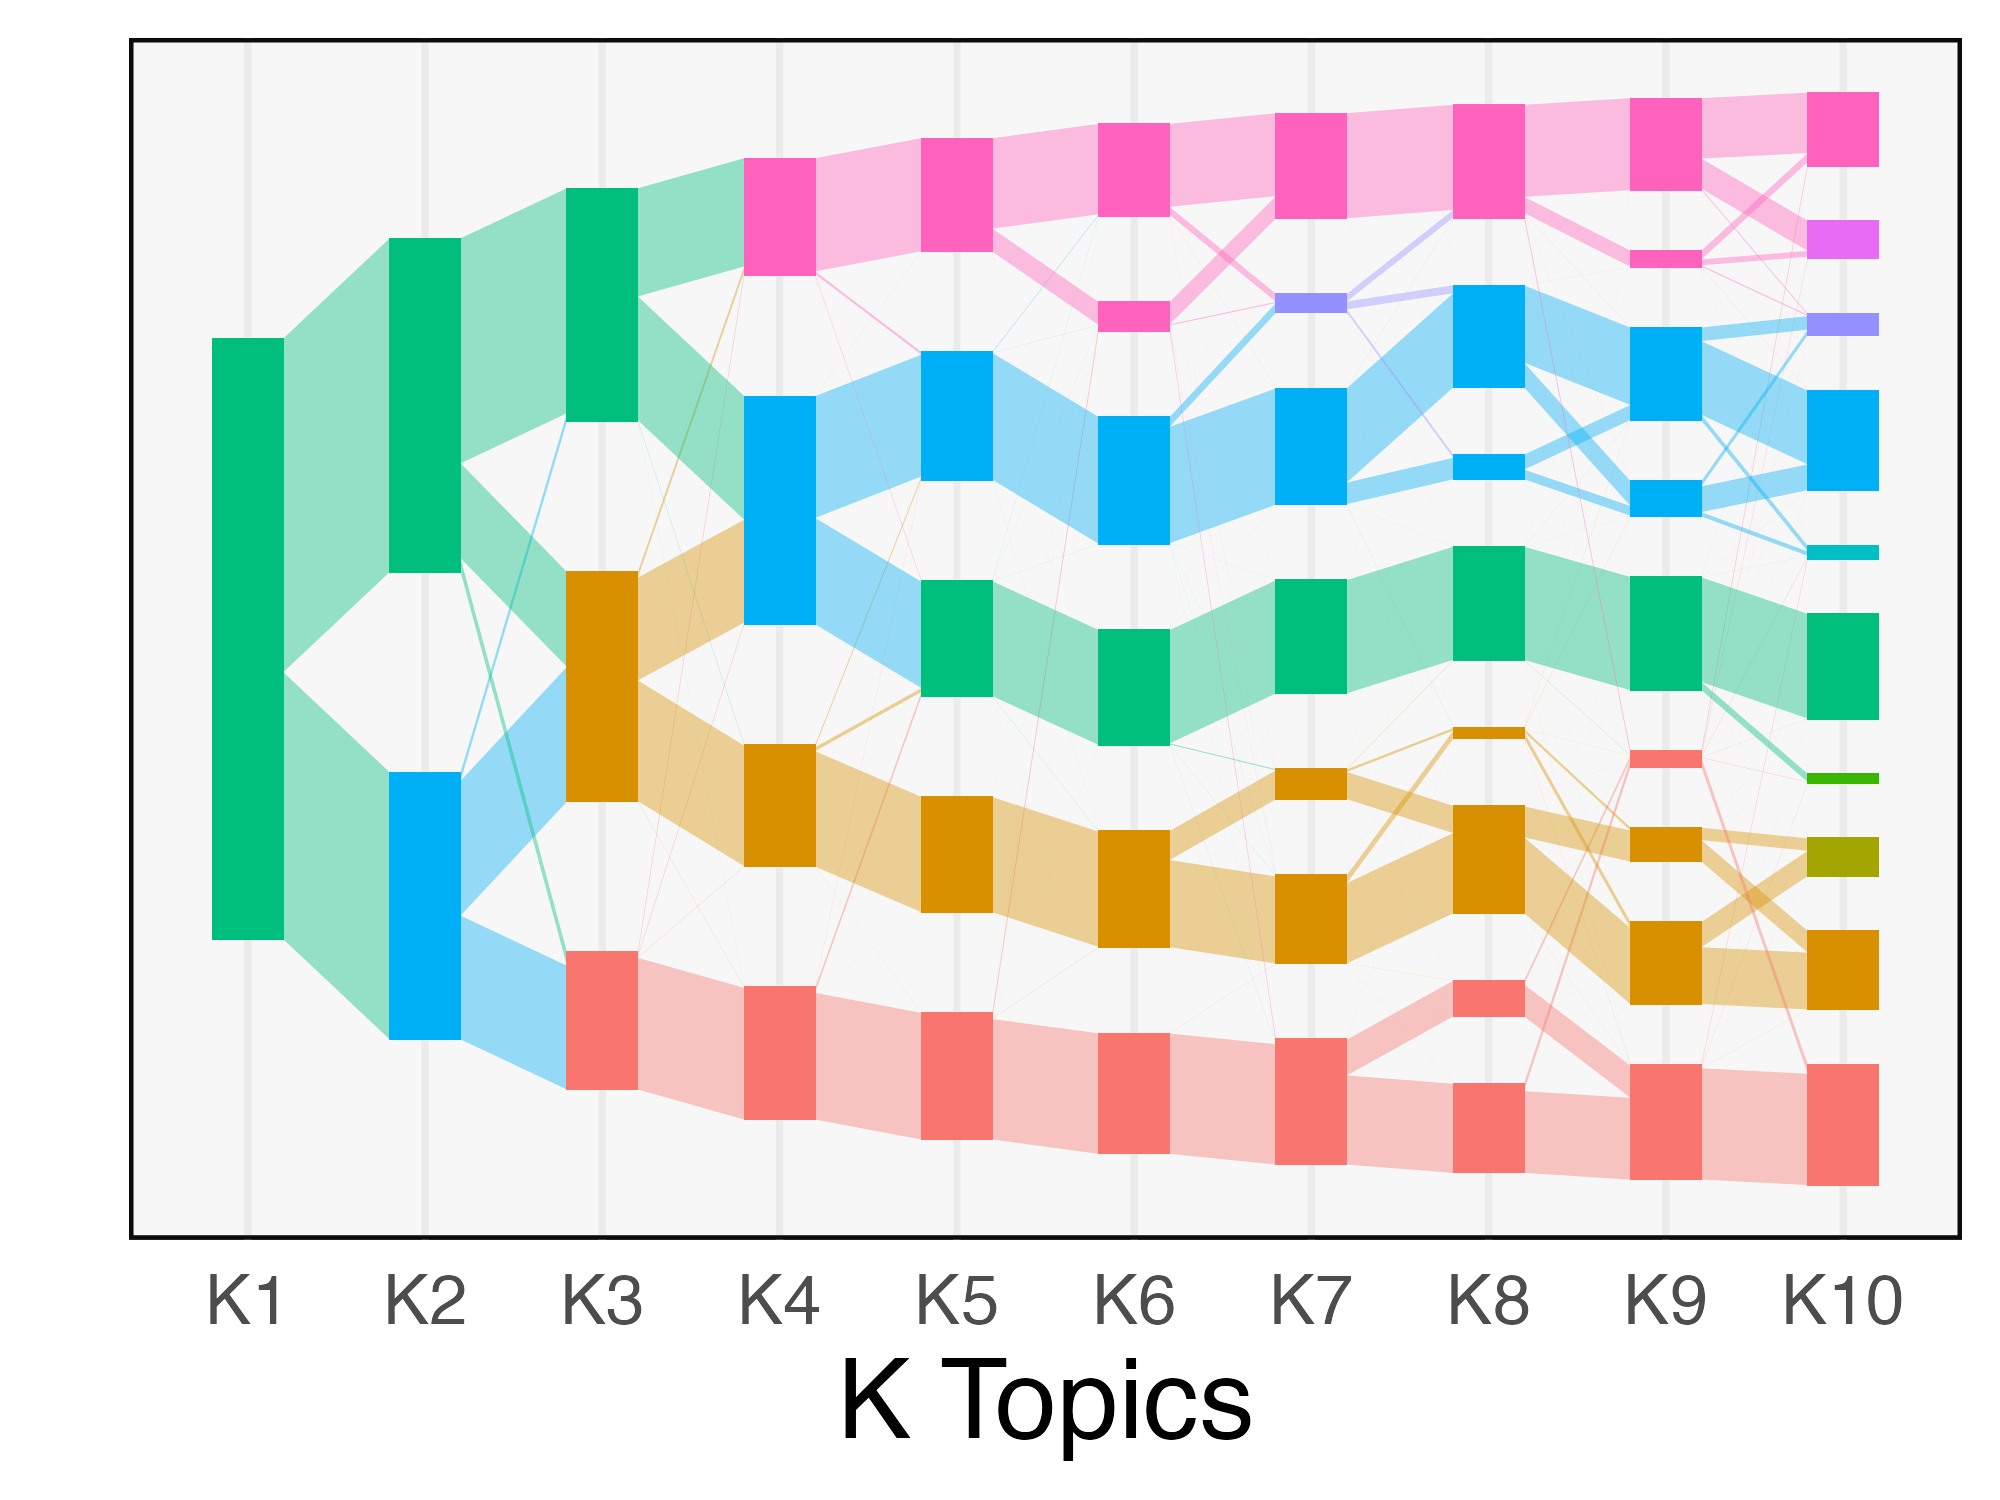
\includegraphics[width=0.35\textwidth]{transport-true-lda}}
    \subfloat{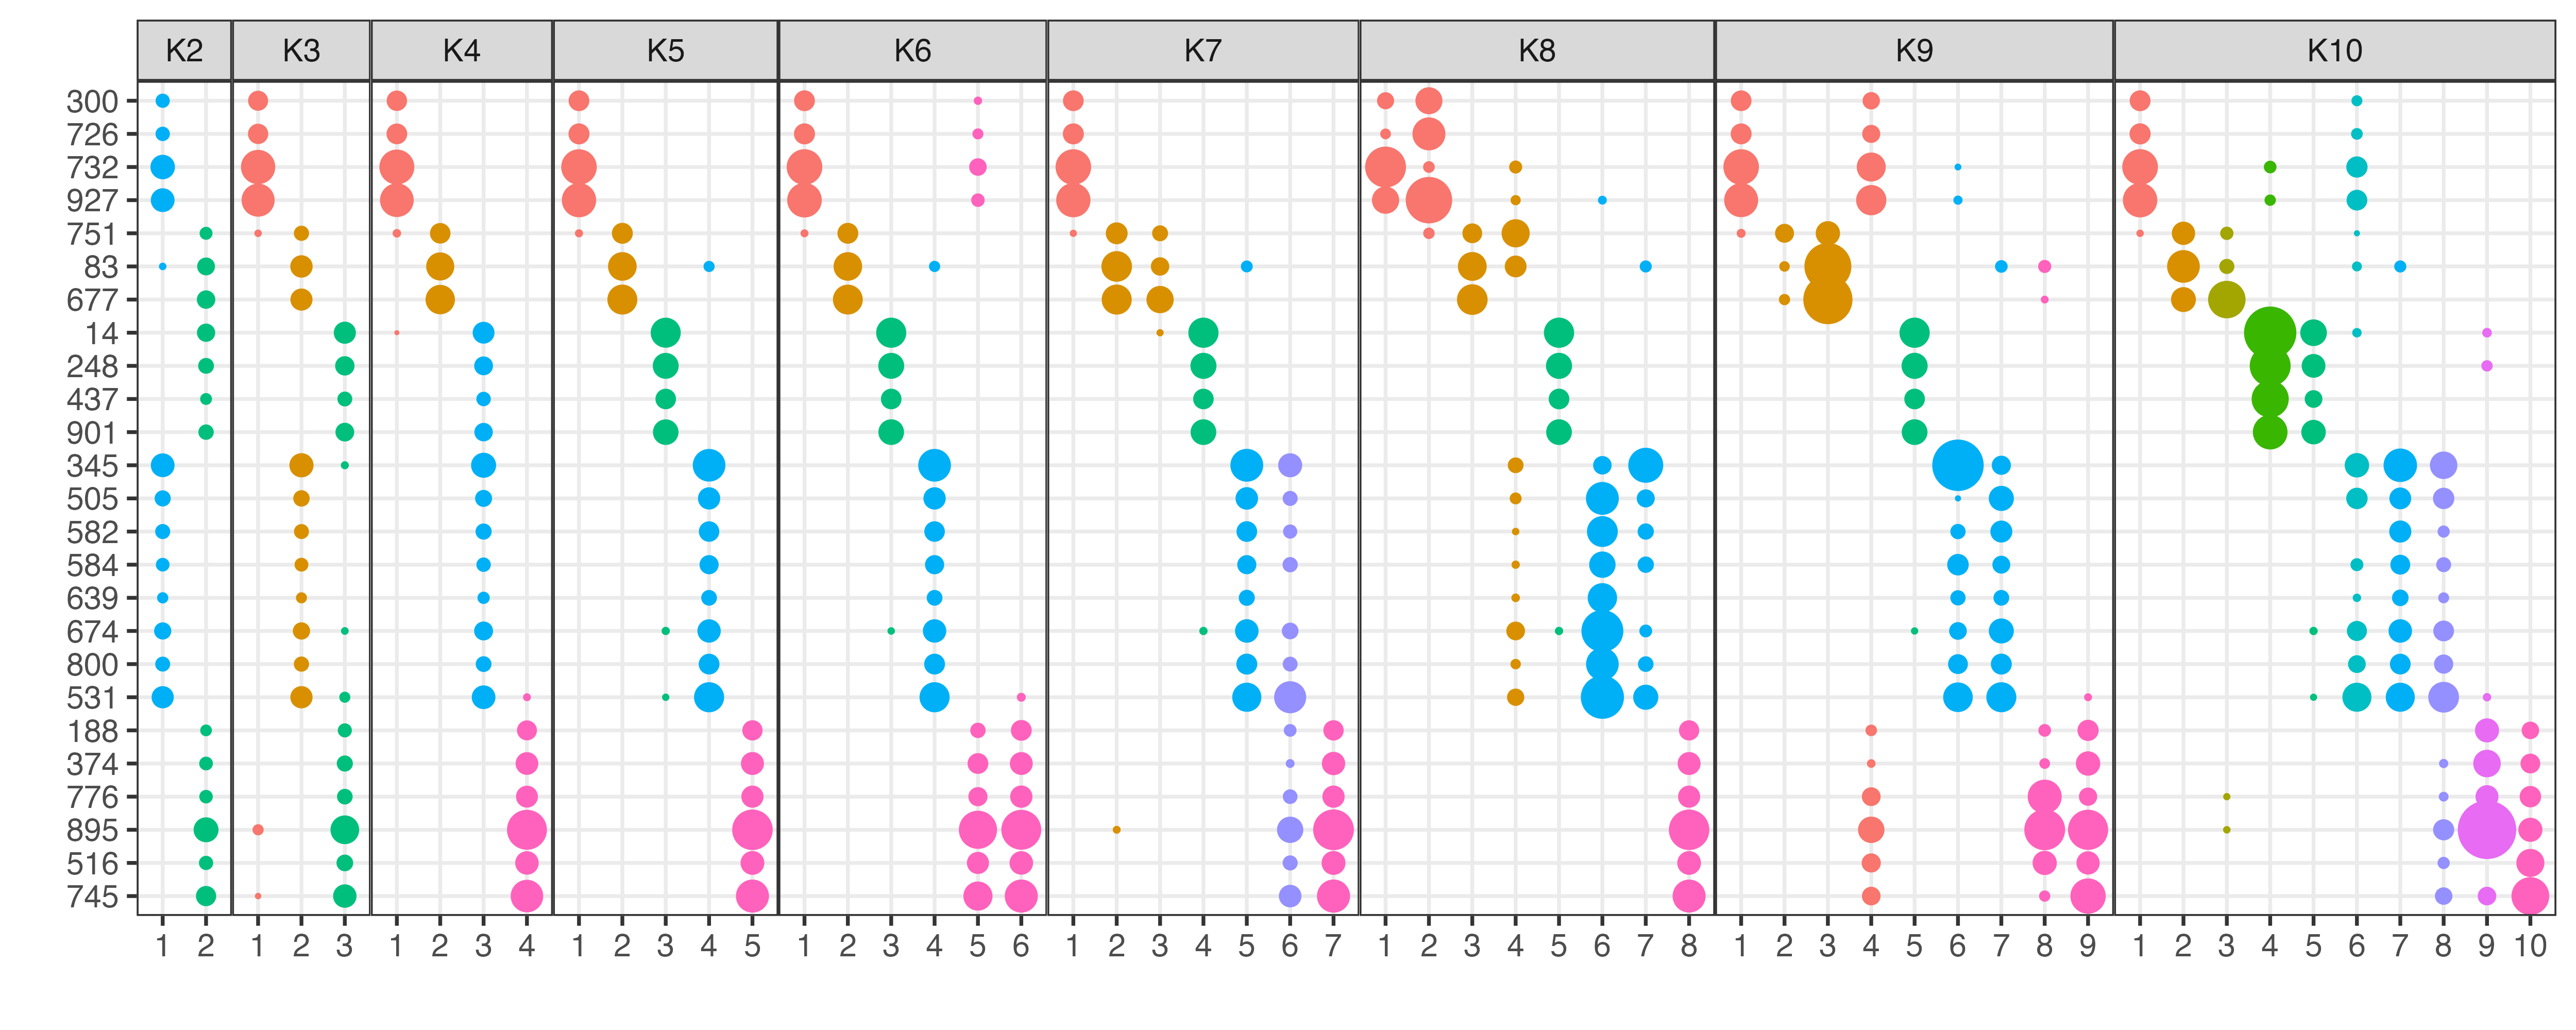
\includegraphics[width=0.63\textwidth]{transport-true-lda-betas}}
\end{figure}
\end{frame}

\section{Methodology}

\begin{frame}
  \frametitle{Topic Models}
  On popular topic model is Latent Dirichlet Allocation (LDA), which supposes
  that each $x_{i}$ is drawn independently according to,
  \begin{align*}
  x_i \vert \gamma_i &\sim \Mult\left(n_{i}, B\gamma_{i}\right) \\
  \gamma_{i} &\sim \Dir\left(\lambda_{\gamma} 1_{K}\right)
  \end{align*}
  where the columns $\beta_{k}$ of $B \in \simplex^{D}$ lie in the $D$
  dimensional simplex and are themselves drawn independently from,
  \begin{align*}
  \beta_{k} \sim \Dir\left(\lambda_{\beta} 1_{D}\right).
\end{align*}
  We will vertically stack the $N$ $\gamma_i$'s into an $N \times K$ matrix
  $\Gamma$.
\end{frame}

\begin{frame}
  \frametitle{Interpretation}
Topic models are well-suited to dimensionality reduction of count data. The
estimated parameters have the following interpretation,
\begin{itemize}
  \item $\Gamma \in \Delta_{K}^{N}$: Per-document memberships across $K$ topics.
  \item $B \in \Delta_{V}^{K}$: Per topic distributions over $V$ words.
\end{itemize}

\begin{figure}
\centering
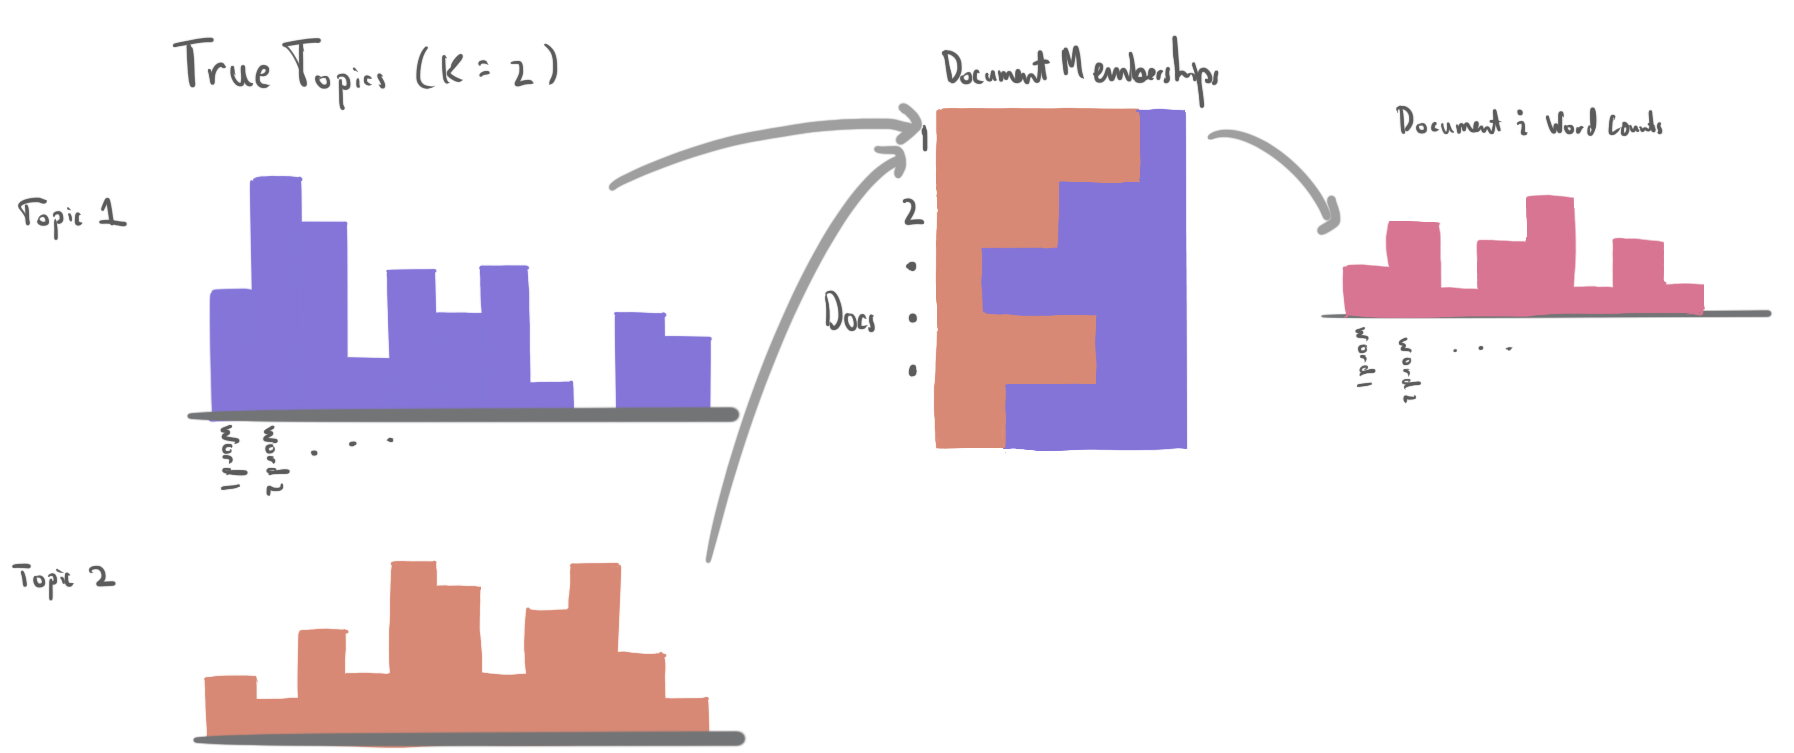
\includegraphics[width=0.9\textwidth]{lda_overview}
\end{figure}
\end{frame}

\begin{frame}
  \frametitle{Alignment as a Graph}
  We view an alignment as a graph across the ensemble. Index models by $m$ and
  topics by $k$. Then,
  \begin{itemize}
    \item Nodes $V$ corresponds to topics, parameterized by $\{\beta^m_{k},
    \gamma^m_{ik}\}$.
    \item Edges $E$ are placed between topics from neighboring models ($K$ vs.
    $K + 1$ topics)
    \item Weights $W$ encode the similarity between topics.
  \end{itemize}
\end{frame}

\begin{frame}
  \frametitle{Notation}
  This graph-based view provides a convenient notation,
  \begin{itemize}
  \item $m\left(v\right)$ is the model for node $v$
  \item $k\left(v\right)$ is the topic for node $v$
  \item $\Gamma\left(v\right) := \left(\gamma_{i
  v\left(k\right)}^m\left(k\right)\right) \in \reals^n_{+}$ is the vector of
  mixed memberships for topic $v$
  \item $\beta\left(v\right) := \beta_{k}^m \in \simplex^{D}$ is the
  corresponding topic distribution
  \item $e = \left(v, v'\right)$ is an edge linking topics $v$ and $v'$.
  \end{itemize}
\end{frame}

\begin{frame}
  \frametitle{$W$ via the product method}
How should we estimate the weights? One idea is to use
\begin{align*}
w\left(e\right) = \Gamma\left(v\right)^T\Gamma\left(v'\right)
\end{align*}
\begin{figure}
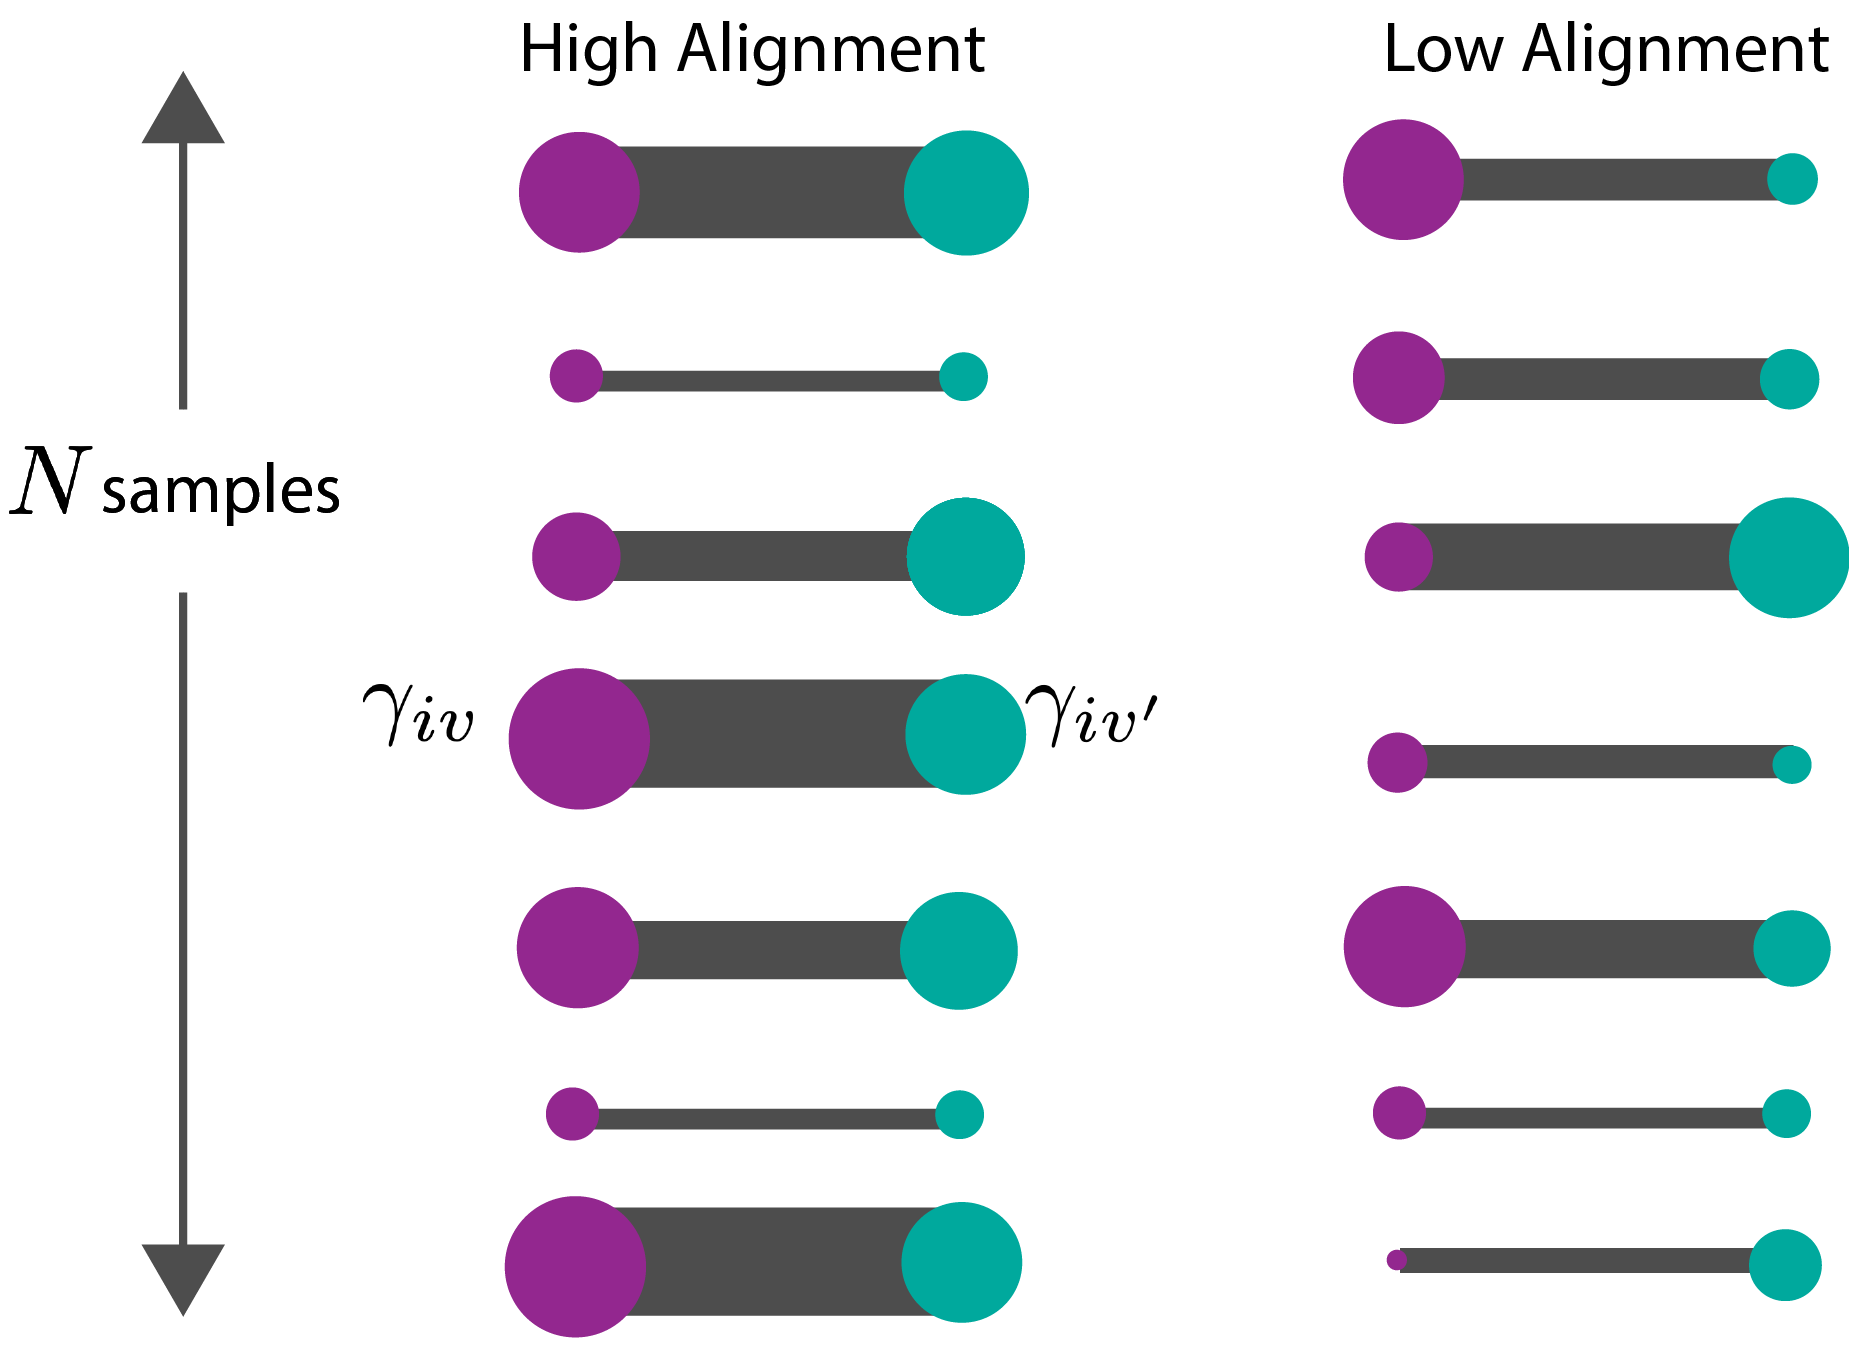
\includegraphics[width=0.6\textwidth]{product_alignment}
\end{figure}
\end{frame}

\begin{frame}
  \frametitle{$W$ via the transport method}
  Let $V_p$ and $V_q$ be two subsets of topics within the graph.
  \begin{itemize}
    \item Let the total ``mass'' of $V_p$ be $p =
    \left\{\Gamma\left(v\right)^T 1 : v \in V_{p}\right\}$. Define $q$ similarly.
    \item Define the transport cost $C\left(v, v^\prime\right) :=
    JSD\left(\beta\left(v\right), \beta\left(v^\prime\right)\right)$, the
    Jensen-Shannon divergence between the pair of topic distributions.
  \end{itemize}
\begin{figure}
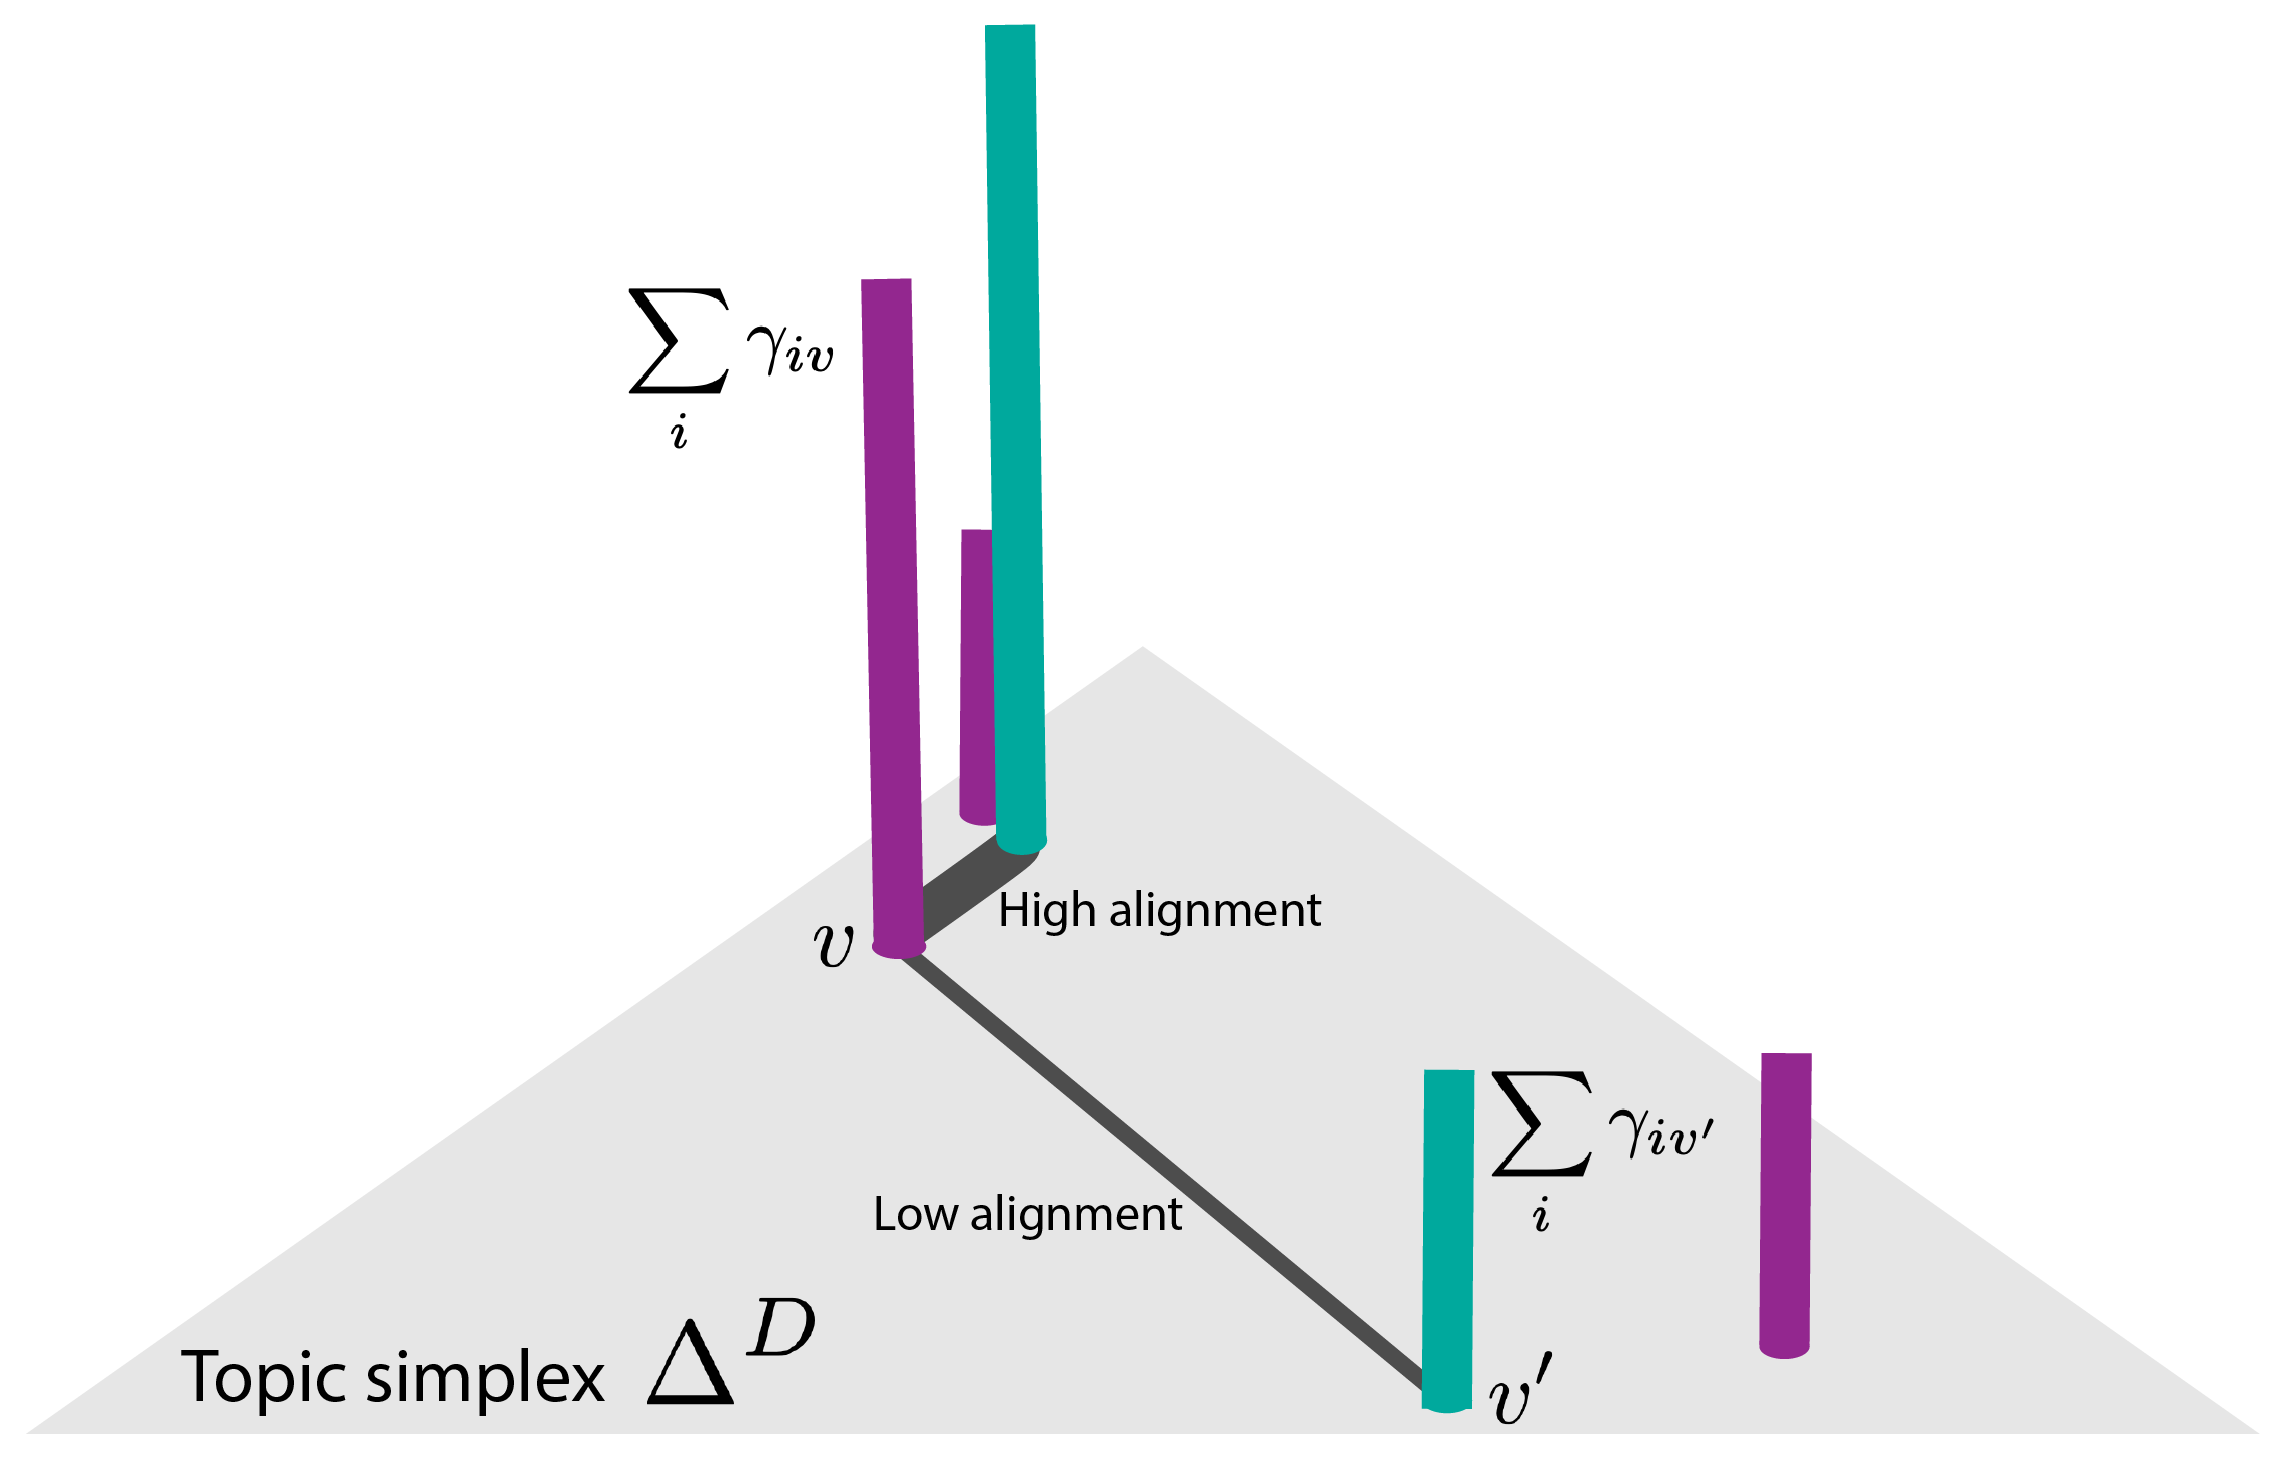
\includegraphics[width=0.7\textwidth]{transport_alignment}
\end{figure}
\end{frame}

\begin{frame}
\frametitle{$W$ via the transport method}
The weights $W$ can than be estimated by solving the optimal transport problem,
\begin{align*}
&\min_{W \in \mathcal{U}\left(p, q\right)} \left<C,W\right> \\
\mathcal{U}\left(p, q\right) := &\{W\in \reals^{\absarg{p} \times \absarg{q}}_{+} : W 1_{\absarg{q}} = p \text{ and } W^{T} 1_{\absarg{p}^\prime} = q\}.
\end{align*}
\begin{figure}
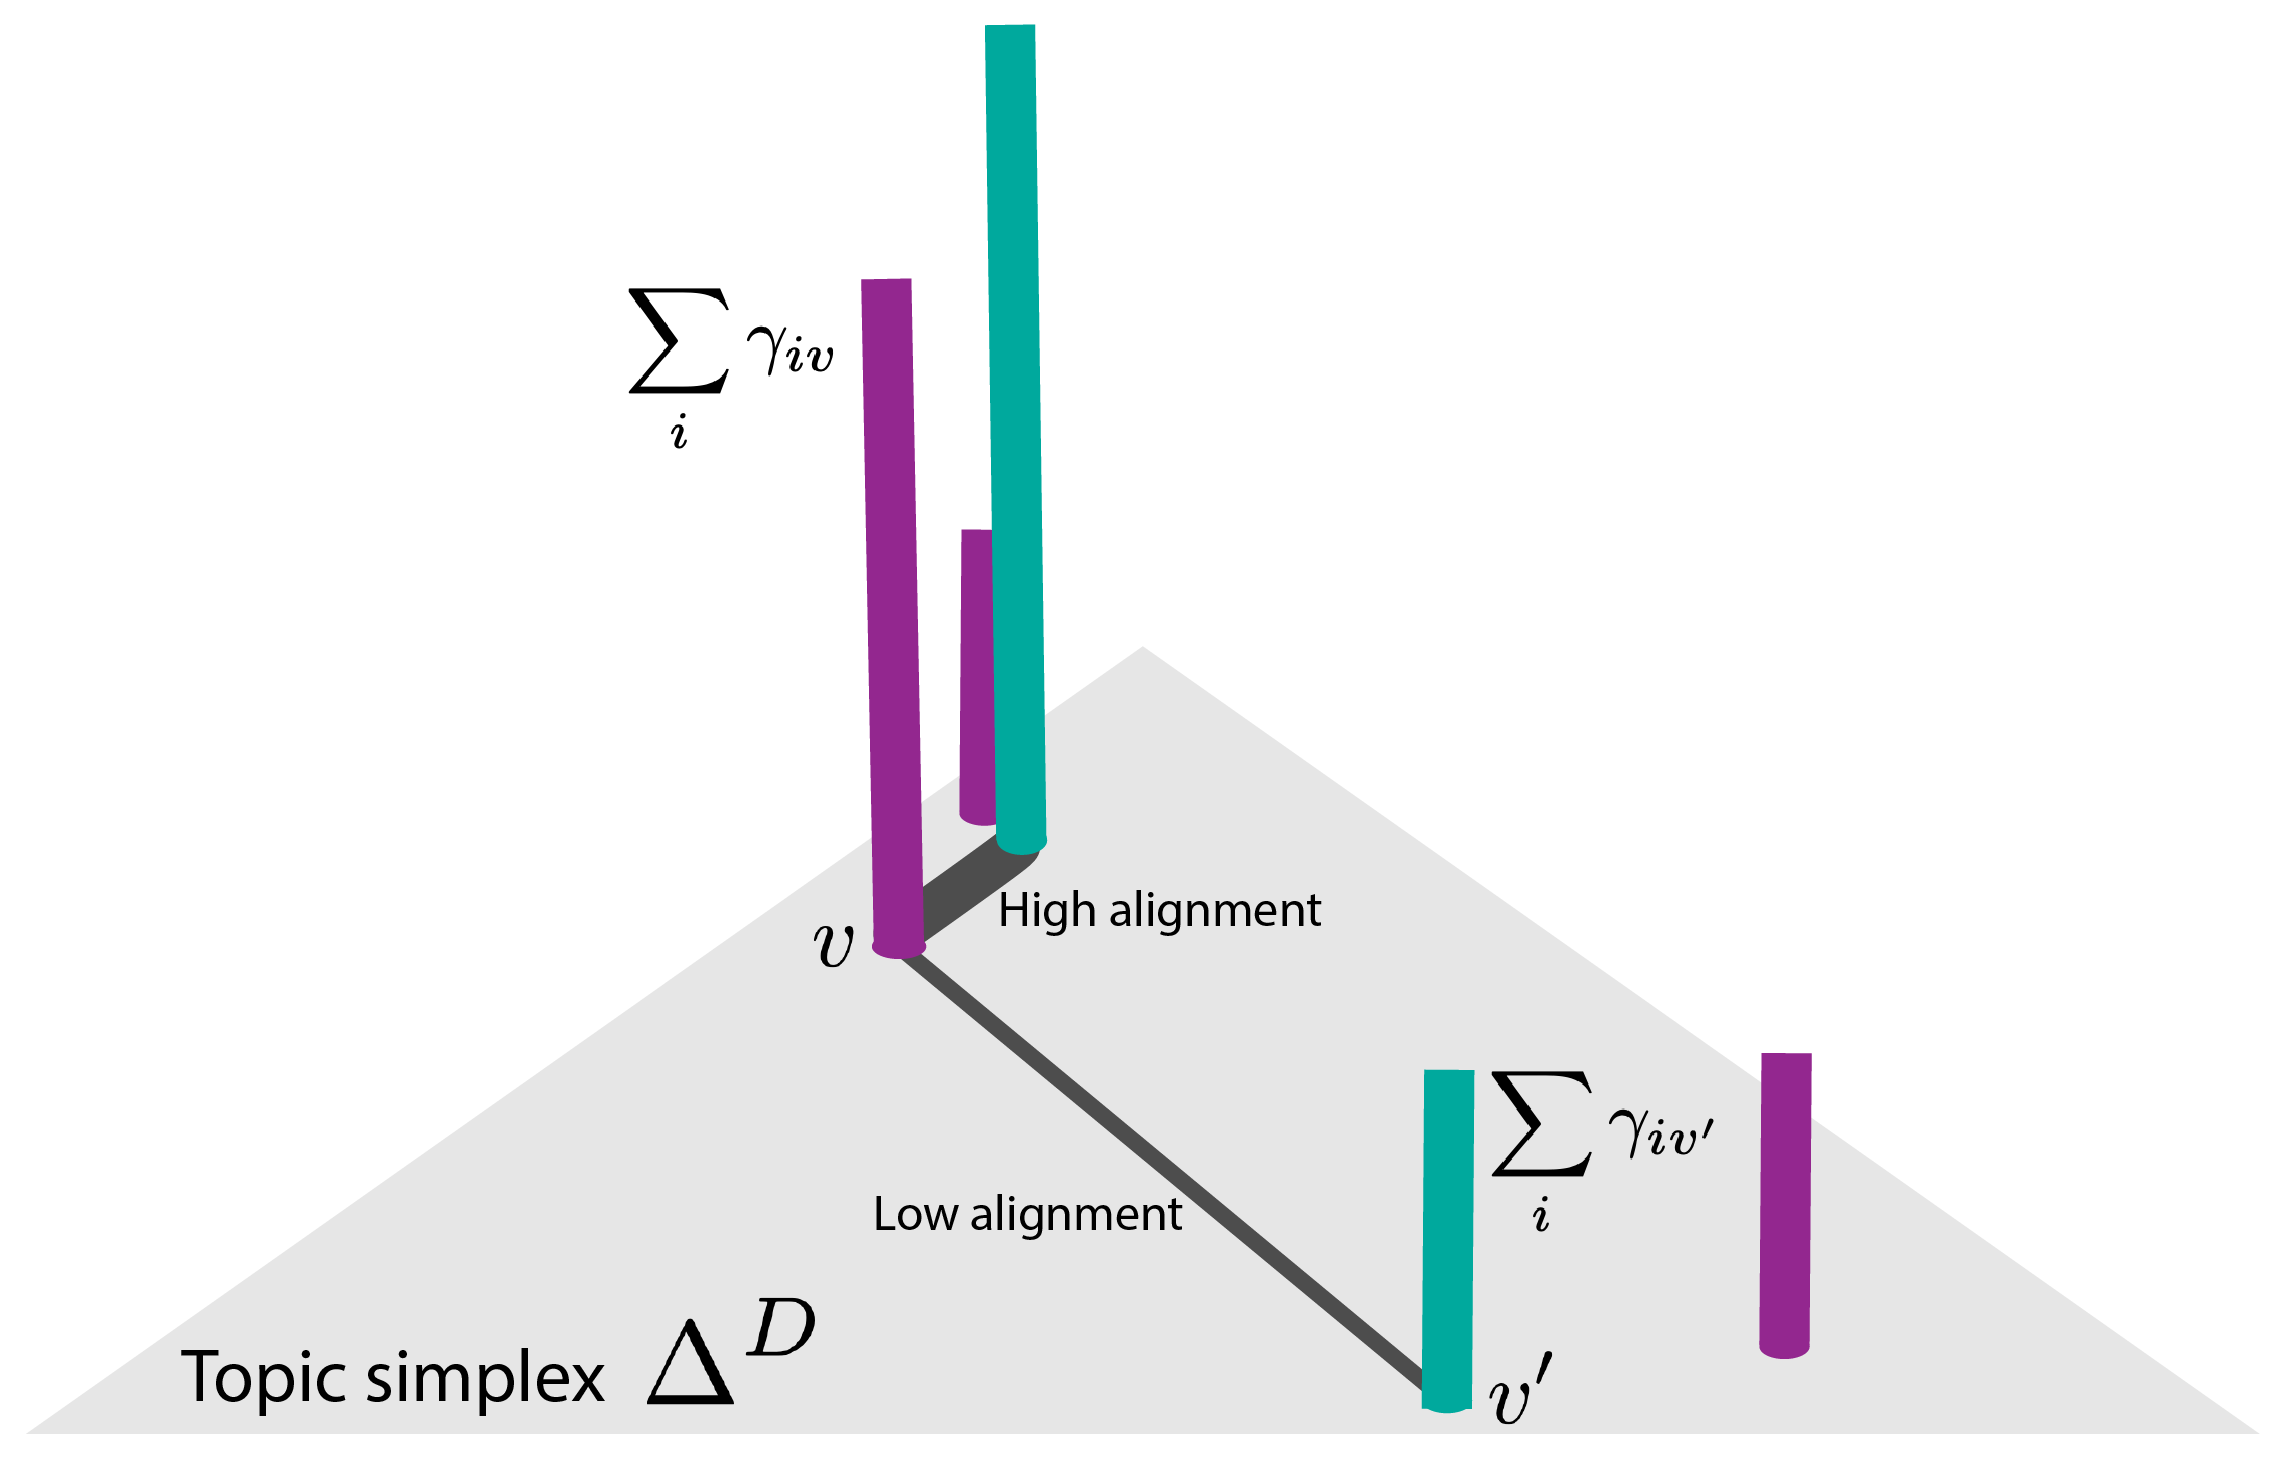
\includegraphics[width=0.7\textwidth]{transport_alignment}
\end{figure}
\end{frame}

\begin{frame}
  \frametitle{Summaries}
  \begin{itemize}
    \item Representing the models by an alignment suggests a few summary measures
    \item These summaries help measure topic quality
    \item They can also be used to diagnose model mis-specification
  \end{itemize}
\end{frame}

\begin{frame}
  \frametitle{Key Topics}
  For each $v$, identify the incoming edge with the highest normalized weight,
  \begin{align*}
    e^\ast\left(v\right) = \arg \max_{e : \text{target}\left(e\right) = v} \tilde{w}_{\text{out}}\left(e\right) + \tilde{w}_{\text{in}}\left(e\right).
  \end{align*}
  \begin{itemize}
    \item Iterate this process from large to small $l$ to construct a set of
    distinct  paths along the alignment
    \item We call the number of unique paths is called the number \emph{key topics}
  \end{itemize}

\begin{figure}
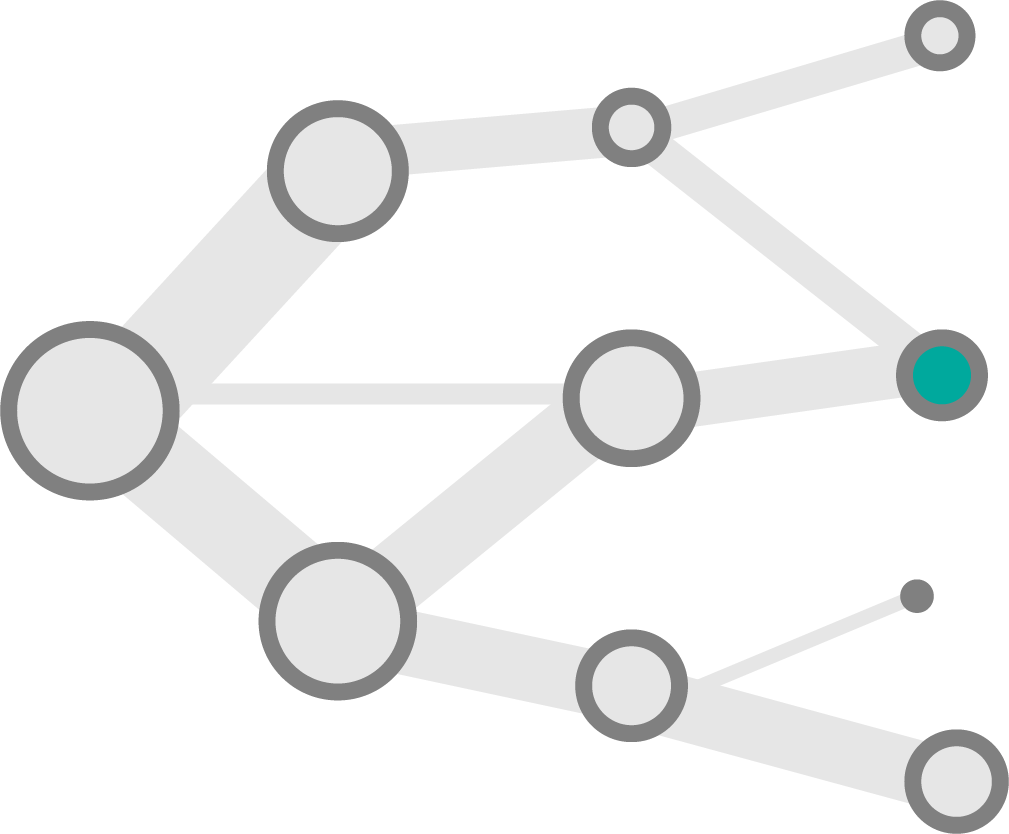
\includegraphics[width=0.4\textwidth]{branch_construction-1}
\end{figure}
\end{frame}

\begin{frame}
  \frametitle{Key Topics}
  For each $v$, identify the incoming edge with the highest normalized weight,
  \begin{align*}
    e^\ast\left(v\right) = \arg \max_{e : \text{target}\left(e\right) = v} \tilde{w}_{\text{out}}\left(e\right) + \tilde{w}_{\text{in}}\left(e\right).
  \end{align*}
  \begin{itemize}
    \item Iterate this process from large to small $l$ to construct a set of
    distinct paths along the alignment
    \item We call the number of unique paths is called the number \emph{key
    topics}
  \end{itemize}

\begin{figure}
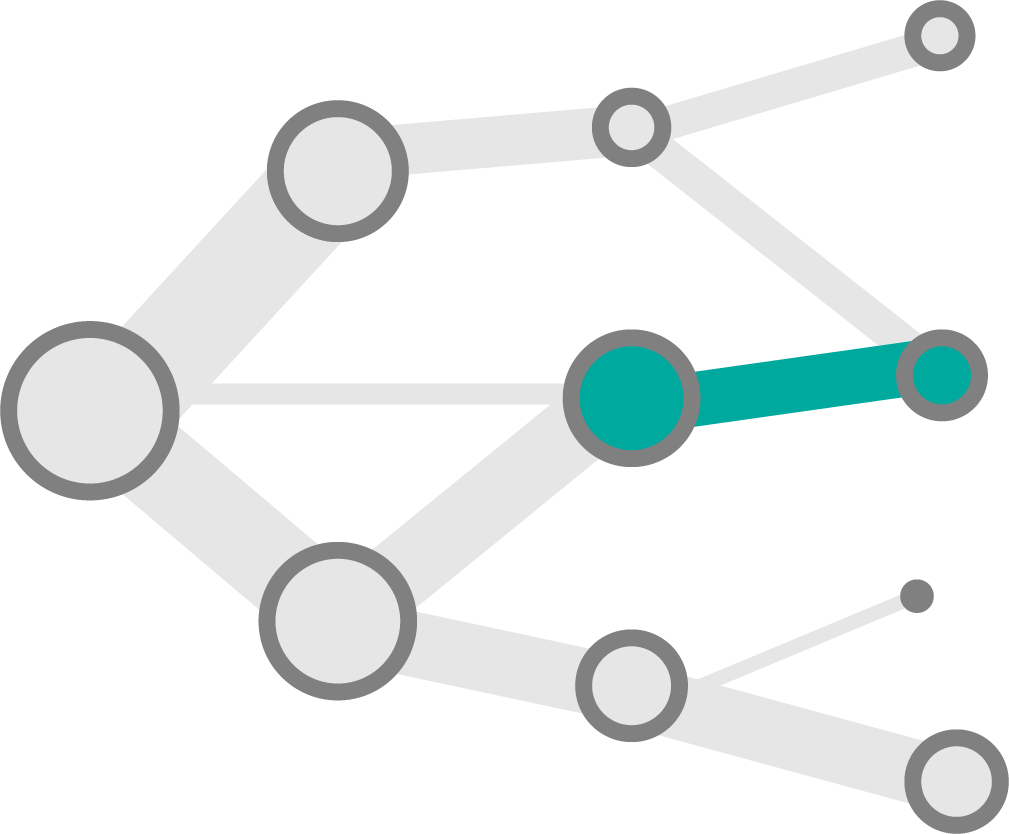
\includegraphics[width=0.4\textwidth]{branch_construction-3}
\end{figure}
\end{frame}

\begin{frame}
  \frametitle{Key Topics}
  For each $v$, identify the incoming edge with the highest normalized weight,
  \begin{align*}
    e^\ast\left(v\right) = \arg \max_{e : \text{target}\left(e\right) = v} \tilde{w}_{\text{out}}\left(e\right) + \tilde{w}_{\text{in}}\left(e\right).
  \end{align*}
  \begin{itemize}
    \item Iterate this process from large to small $l$ to construct a set of
    distinct paths along the alignment
    \item We call the number of unique paths is called the number \emph{key
    topics}
  \end{itemize}

\begin{figure}
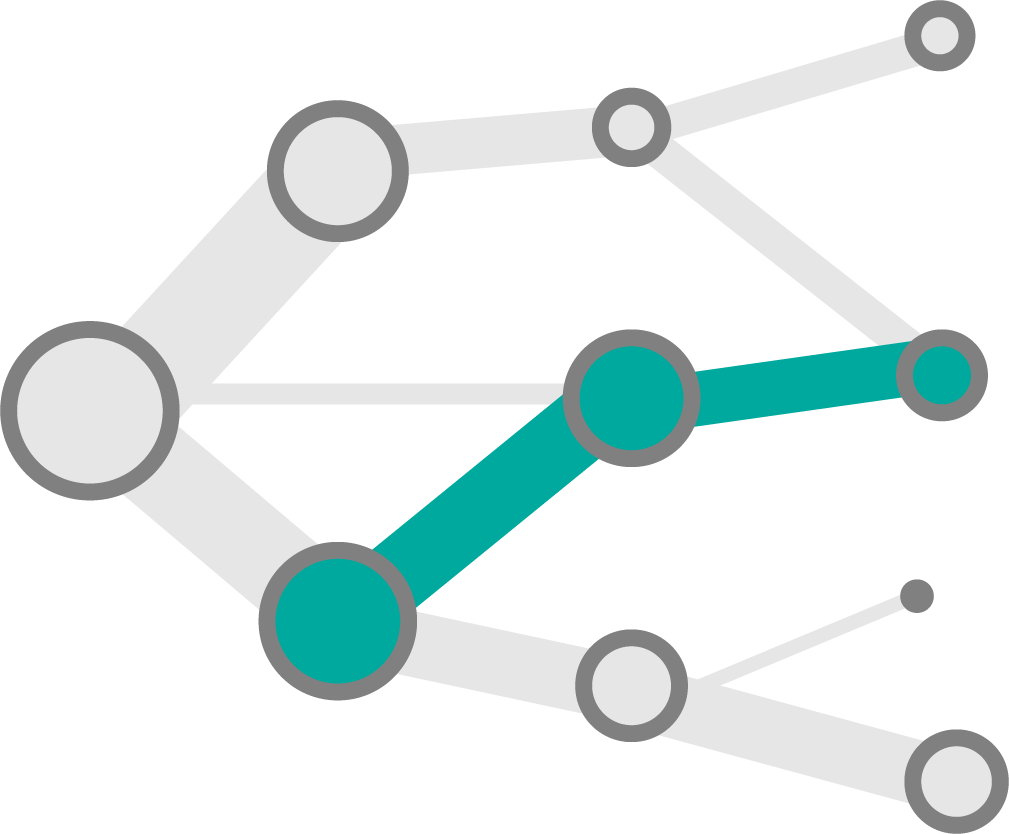
\includegraphics[width=0.4\textwidth]{branch_construction-2}
\end{figure}
\end{frame}

\begin{frame}
  \frametitle{Key Topics}
  For each $v$, identify the incoming edge with the highest normalized weight,
  \begin{align*}
    e^\ast\left(v\right) = \arg \max_{e : \text{target}\left(e\right) = v} \tilde{w}_{\text{out}}\left(e\right) + \tilde{w}_{\text{in}}\left(e\right).
  \end{align*}
  \begin{itemize}
    \item Iterate this process from large to small $l$ to construct a set of
    distinct paths along the alignment
    \item We call the number of unique paths is called the number \emph{key
    topics}
  \end{itemize}

\begin{figure}
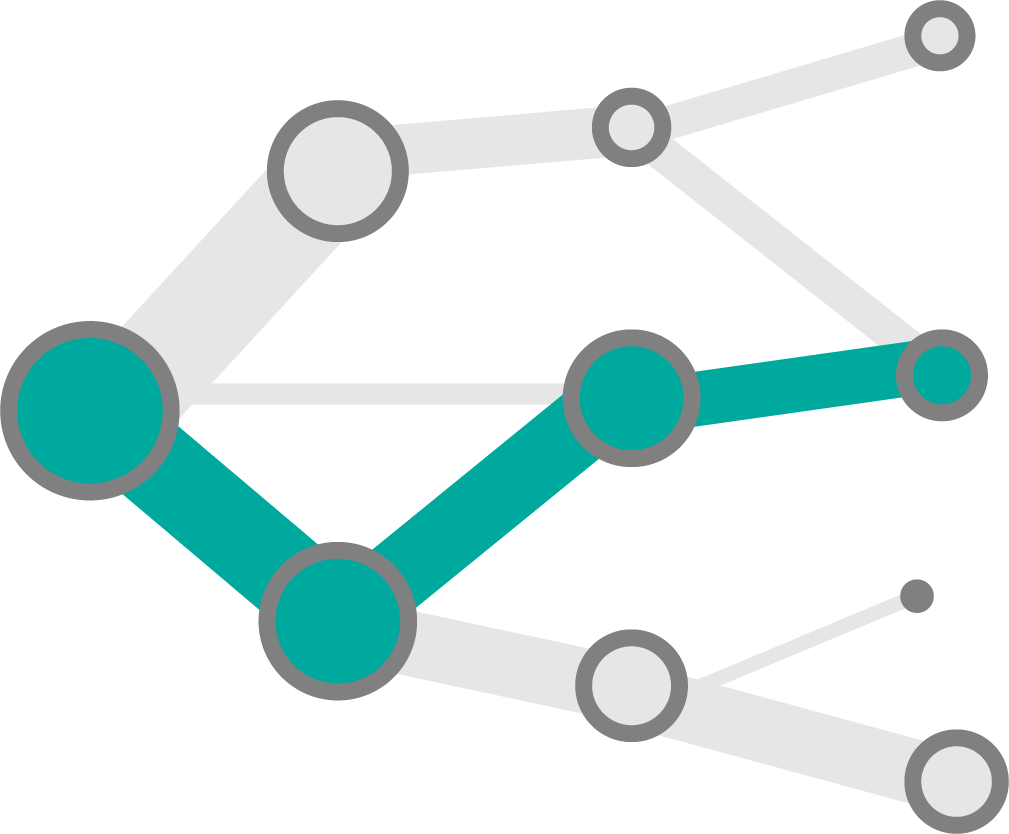
\includegraphics[width=0.4\textwidth]{branch_construction-4}
\end{figure}
\end{frame}


\begin{frame}
  \frametitle{Key Topics}
  For each $v$, identify the incoming edge with the highest normalized weight,
  \begin{align*}
    e^\ast\left(v\right) = \arg \max_{e : \text{target}\left(e\right) = v} \tilde{w}_{\text{out}}\left(e\right) + \tilde{w}_{\text{in}}\left(e\right).
  \end{align*}
  \begin{itemize}
    \item Iterate this process from large to small $l$ to construct a set of
    distinct paths along the alignment
    \item We call the number of unique paths is called the number \emph{key
    topics}
  \end{itemize}

\begin{figure}
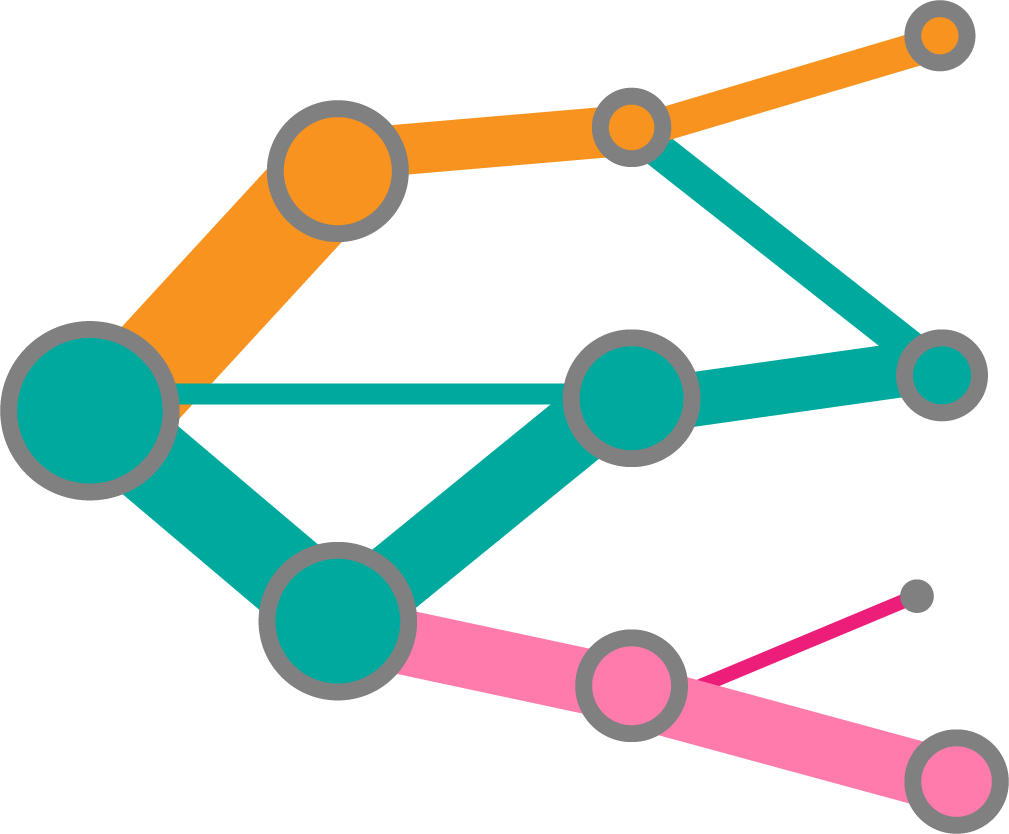
\includegraphics[width=0.4\textwidth]{branch_construction-5}
\end{figure}
\end{frame}


\begin{frame}
  \frametitle{Refinement}
  Suppose there are actually $K_0$ topics in the data. If we fit a model with
  $K$ topics, then
  \begin{itemize}
    \item $K < K_0$: True topics are merged together into ``compromise'' topics
    \item $K > K_0$: True topics are arbitrarily split
  \end{itemize}
\end{frame}

\begin{frame}
  \frametitle{Refinement}
  A consequence is that the parent specificity differs between these
  regimes,
  \begin{itemize}
    \item $K < K_0$: Each topic receives most mass from a unique parent,
    corresponding to a true or ``compromise'' topic
    \item $K > K_0$: Each topic receives substantial mass from several parents,
    each corresponding to an arbitrary split of a true topic
  \end{itemize}

  \begin{figure}
\subfloat{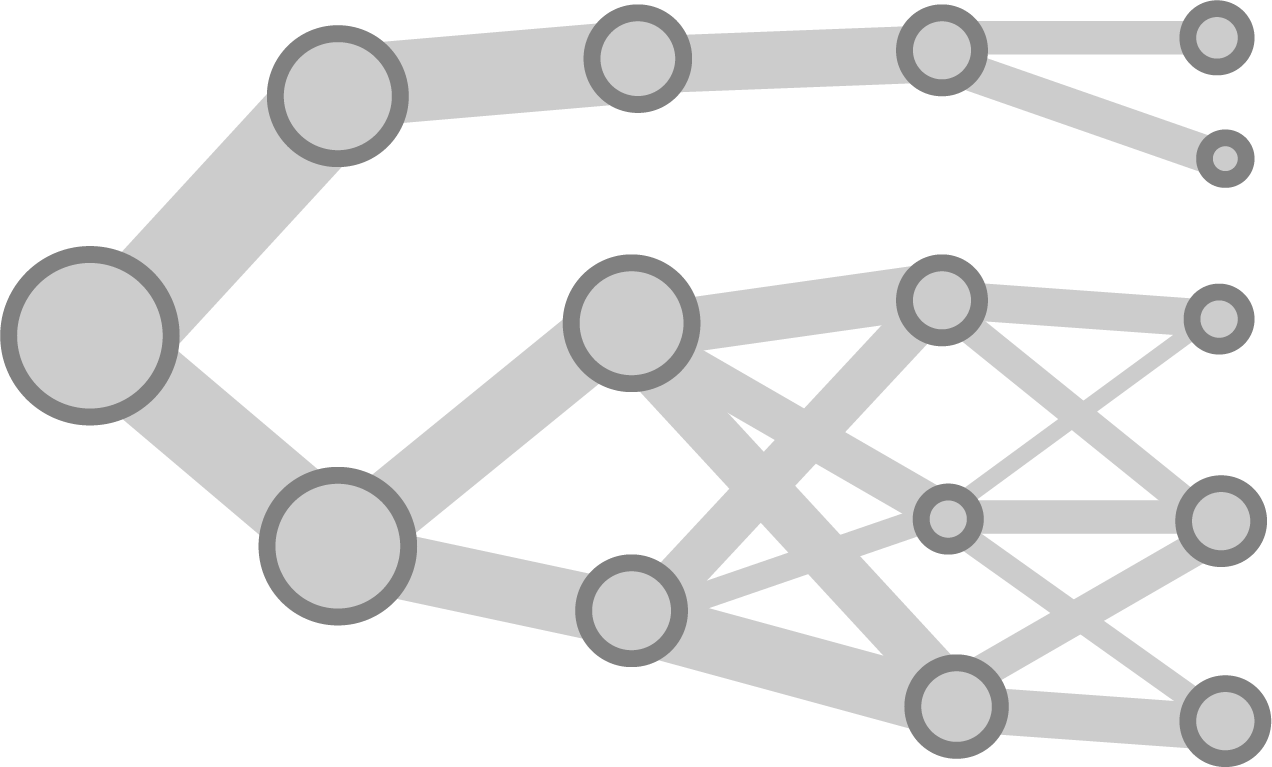
\includegraphics[width=0.3\textwidth]{refinement-branches-2}}$\medspace\medspace\medspace$
\subfloat{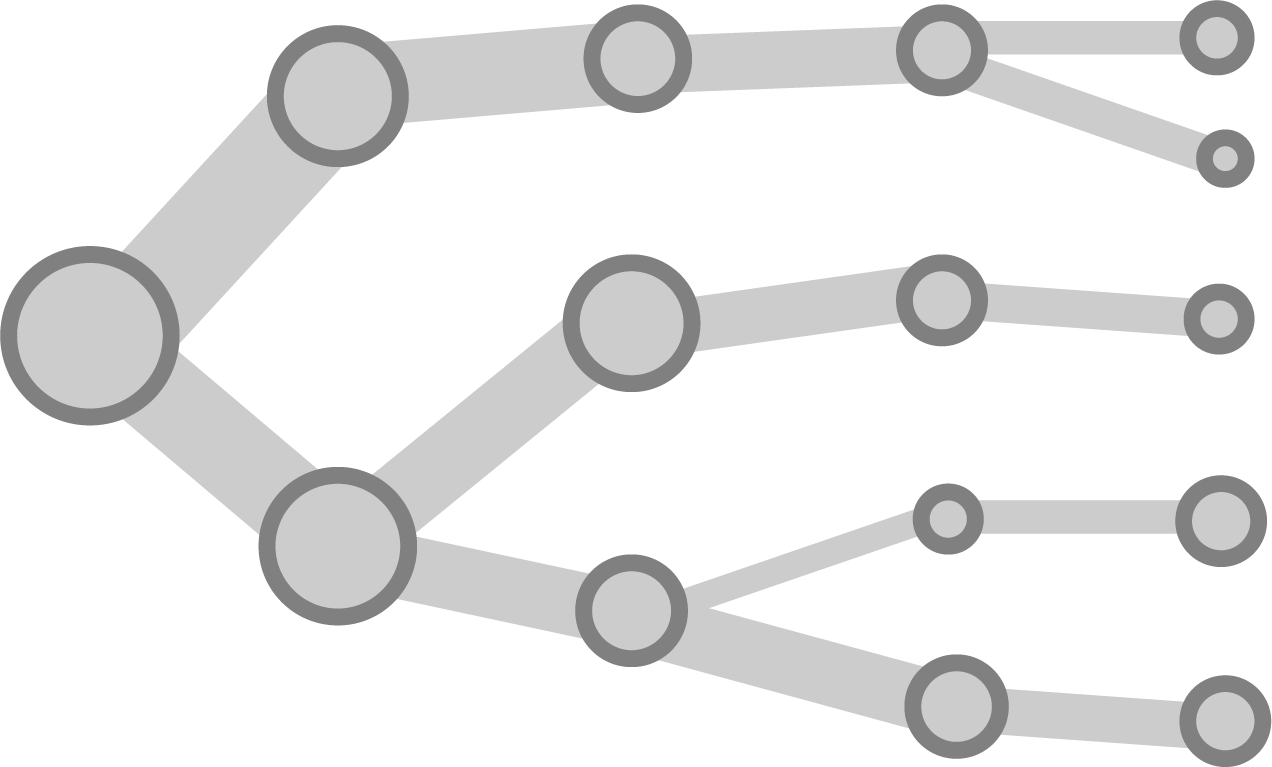
\includegraphics[width=0.3\textwidth]{refinement-branches}}
  \end{figure}

\end{frame}

\begin{frame}
  \frametitle{Coherence}
  The coherence of a topic is defined as its average connectedness to other
  topics along the same branch,
  \begin{align*}
    c(v) = \frac{1}{|\text{Path}\left(v\right)|} \sum_{v' \in \text{Path}\left(v\right)} \min\left(\win\left(v, v'\right), \wout\left(v, v'\right) \right)
  \end{align*}
  \begin{itemize}
    \item Topics that are transient (appearing at one $K$ and disappearing at
    another) have low coherence scores
    \item Topics that are consistently recovered across choices of $K$ have high
    coherence
  \end{itemize}

\end{frame}

\section{Simulations}

\begin{frame}
  \frametitle{True LDA Model}
  A sanity check is compute the alignment of data that are in fact generated by an
  LDA model (true $K = 5$).
  \begin{itemize}
  \item $N = 250, D = 1000, \lambda_{\gamma} = 0.5, \lambda_{\beta} = 0.1$
  \end{itemize}

  \begin{figure}
    \subfloat{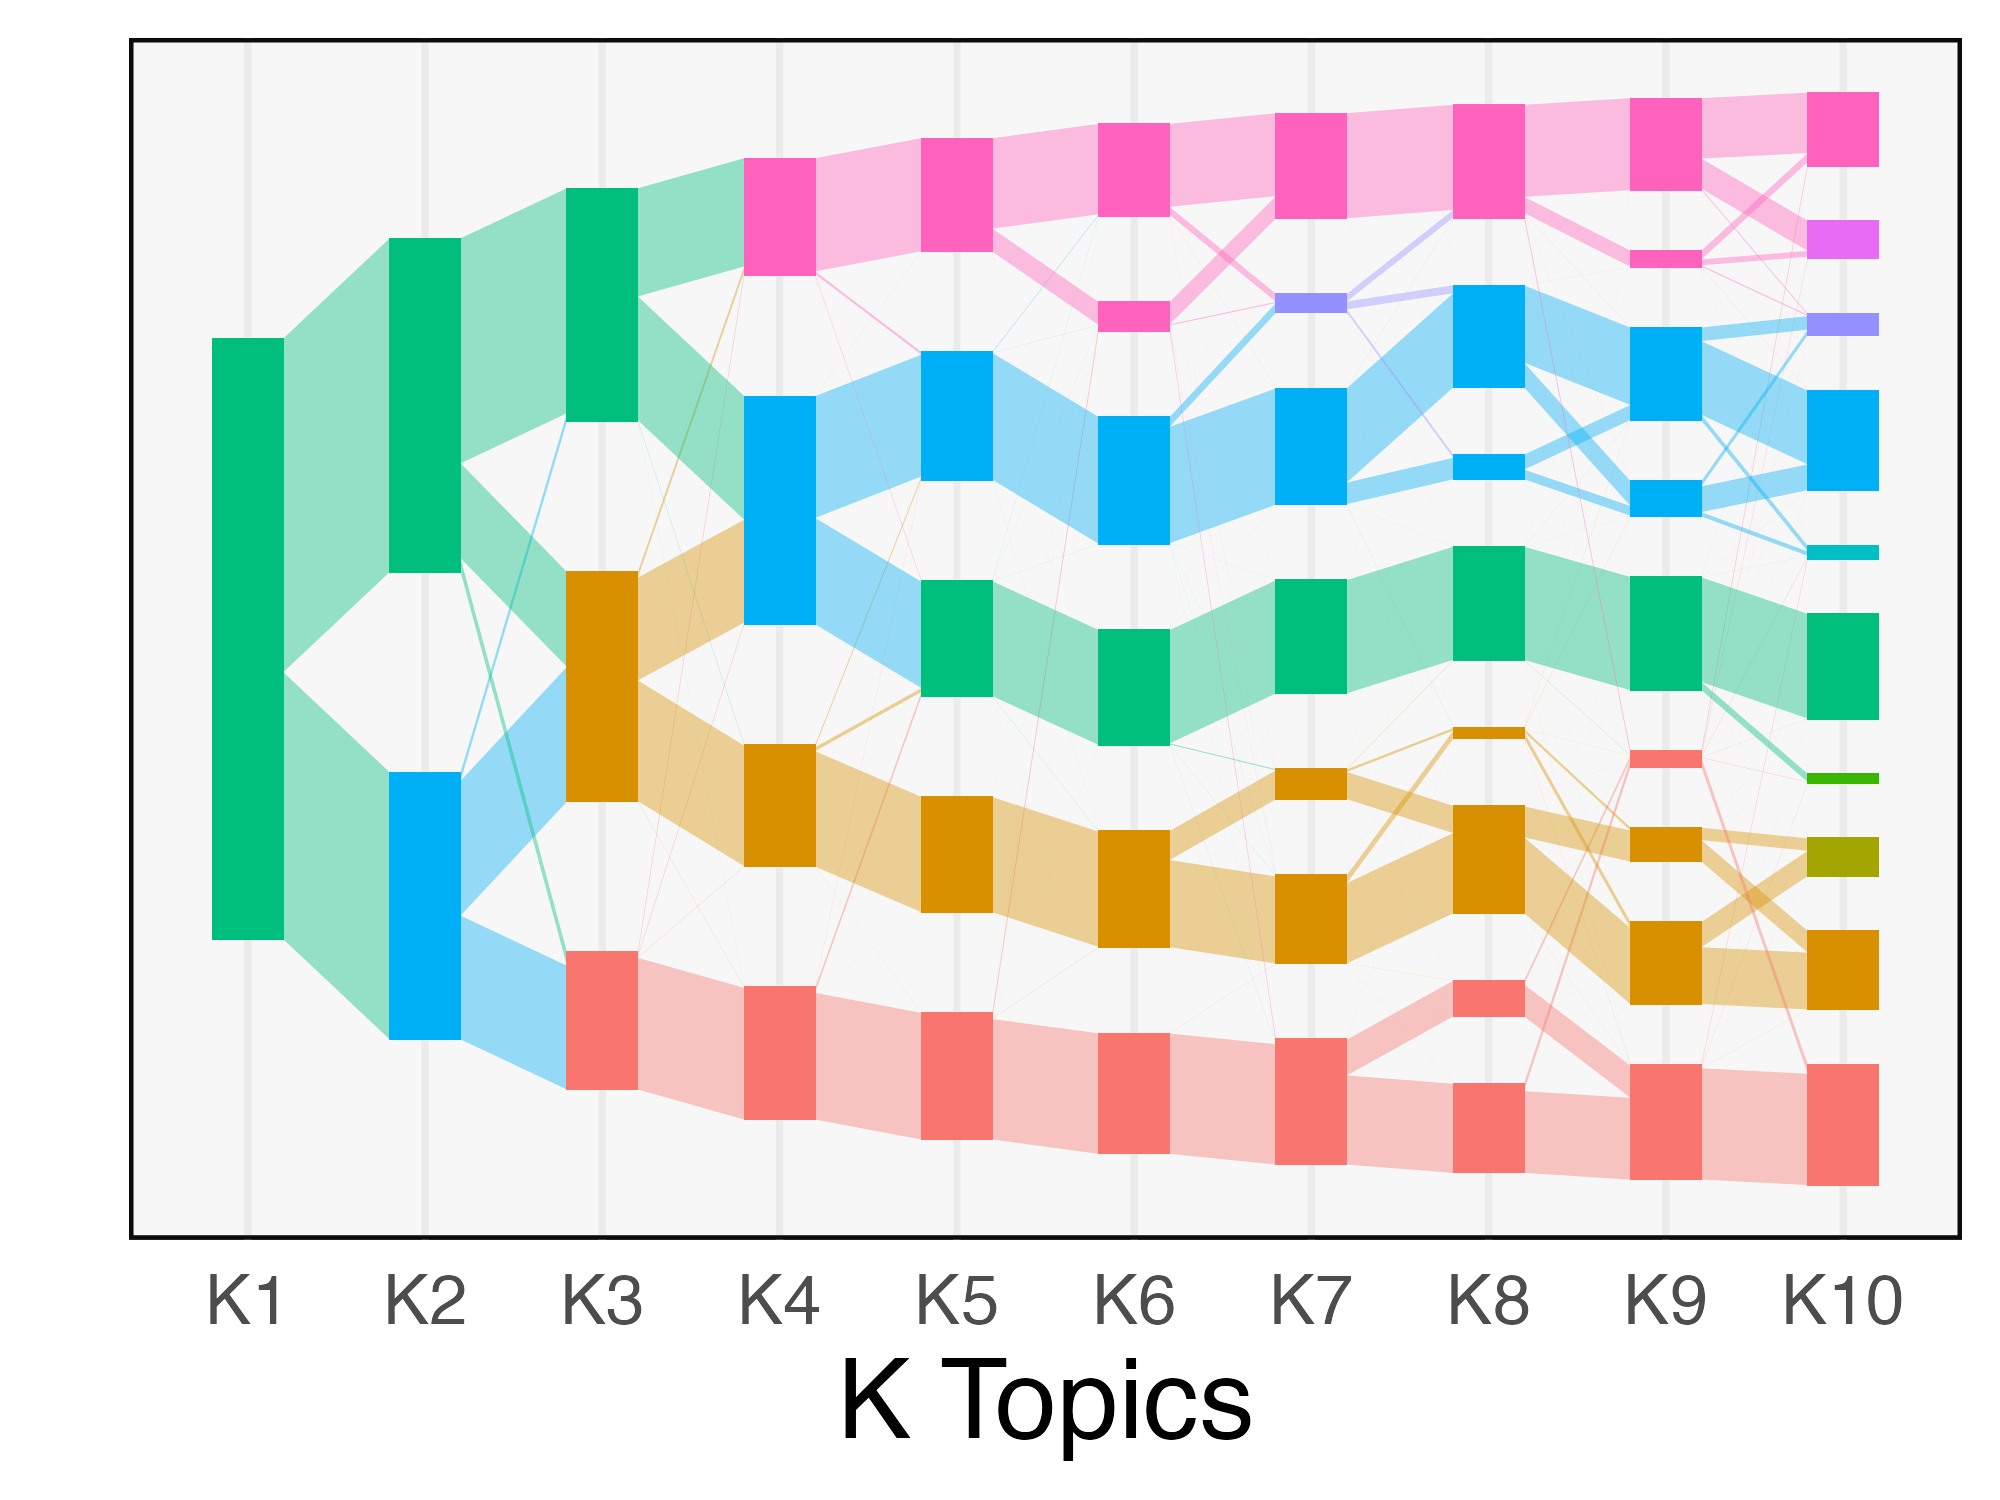
\includegraphics[width=0.4\textwidth]{transport-true-lda}}
    \subfloat{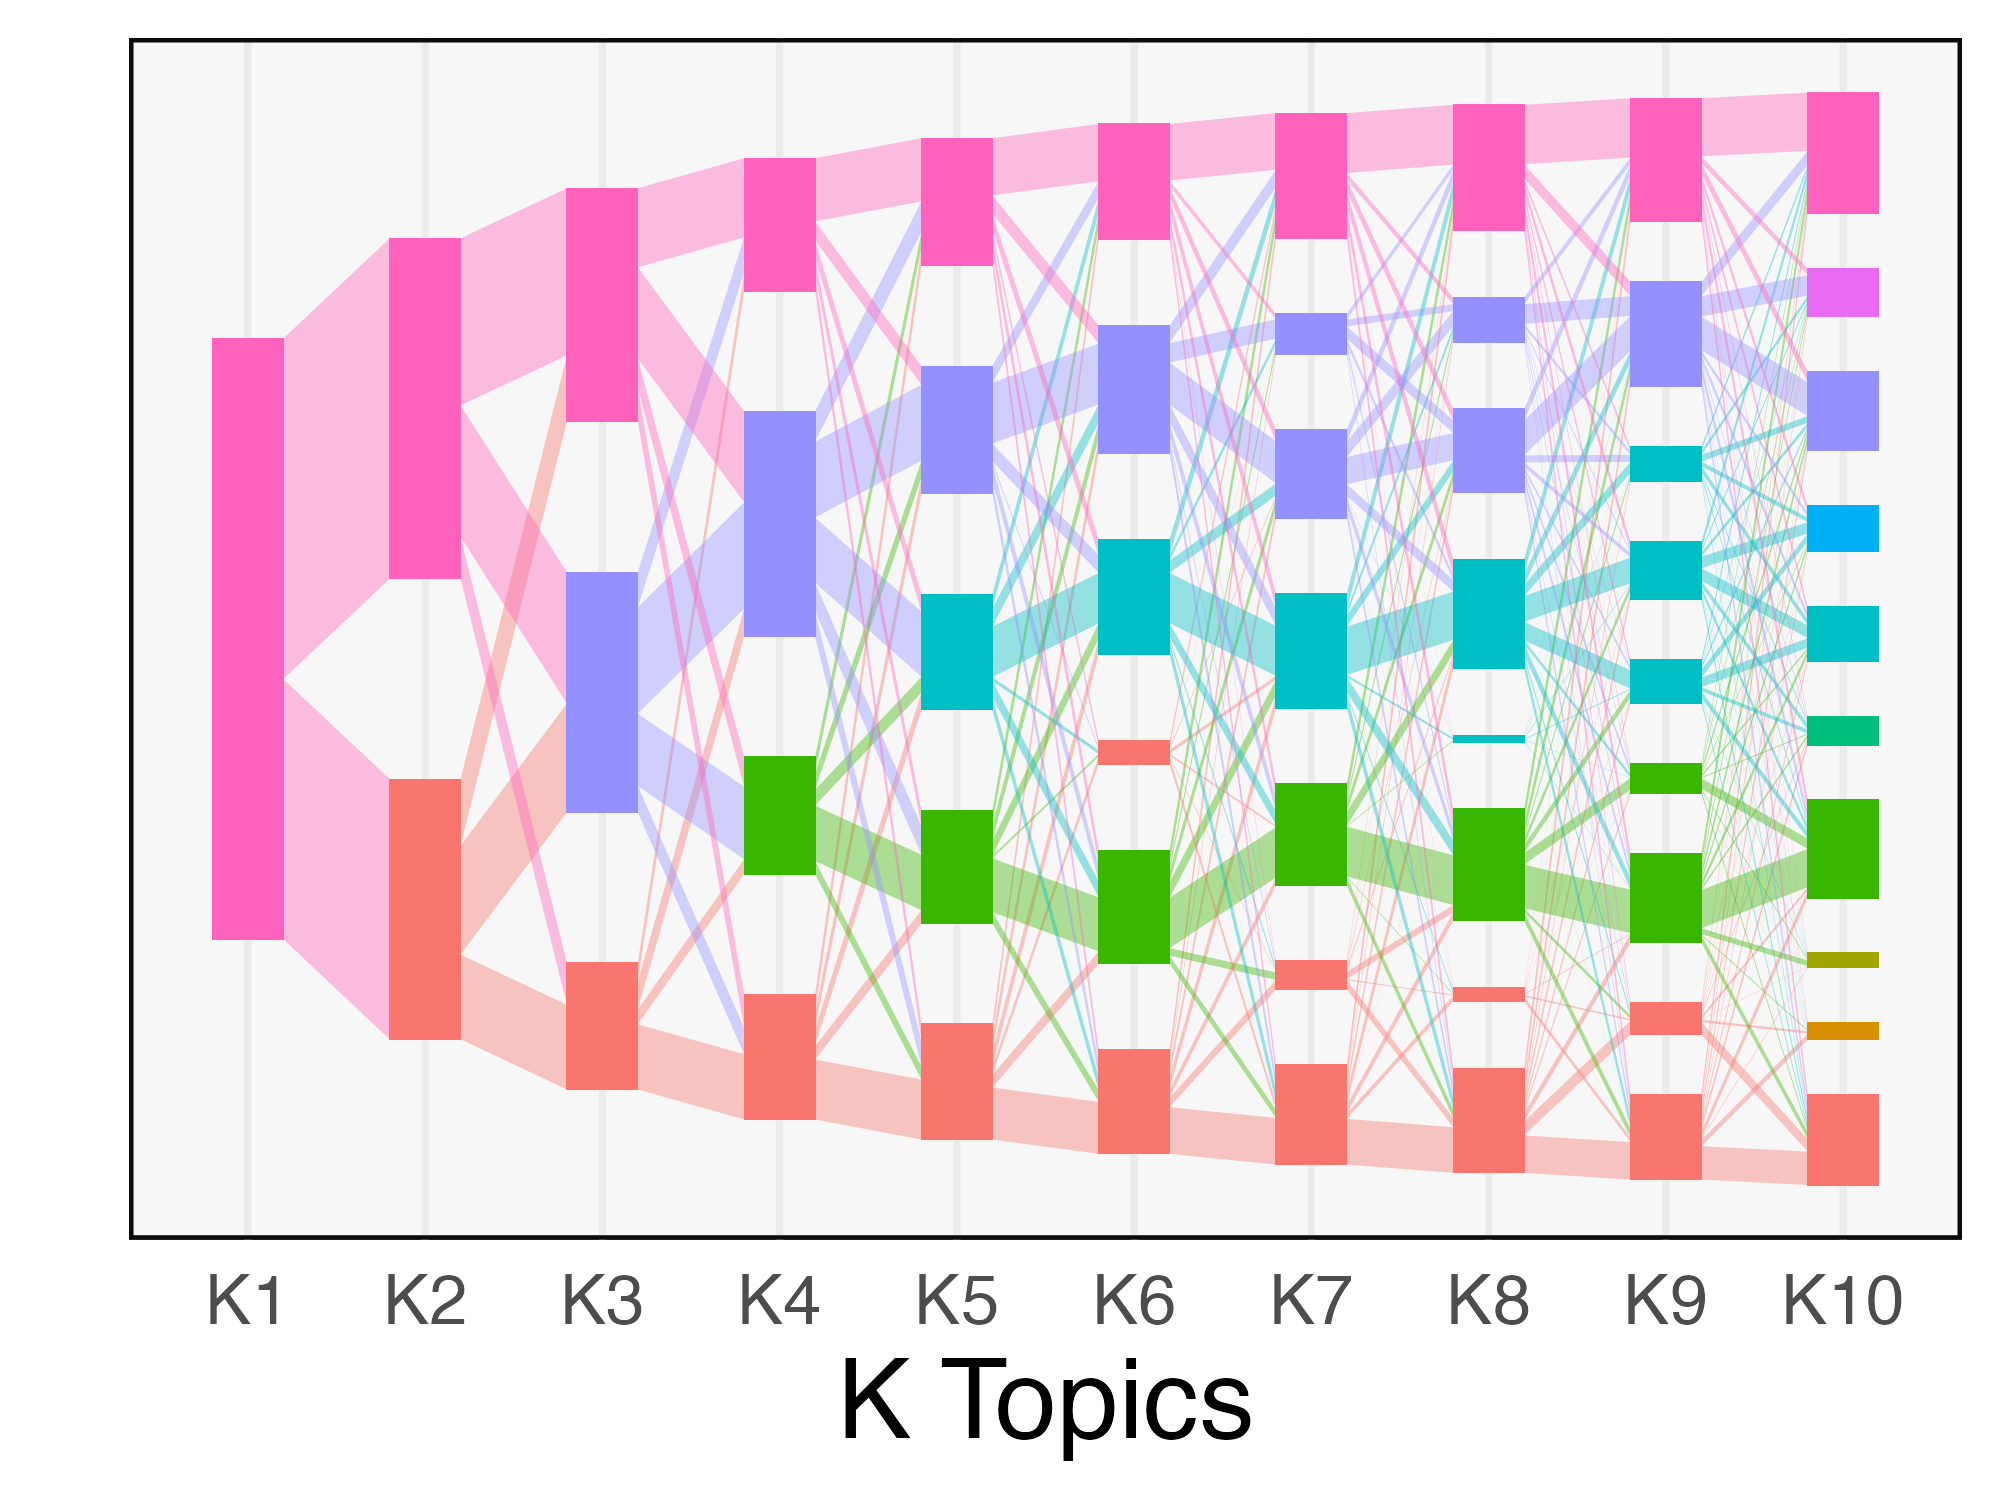
\includegraphics[width=0.4\textwidth]{product-true-lda}}
  \end{figure}
\end{frame}

\begin{frame}
  \frametitle{Summaries}
  The summary measures suggest that the true $K$ is 5.
  \begin{figure}
    \subfloat{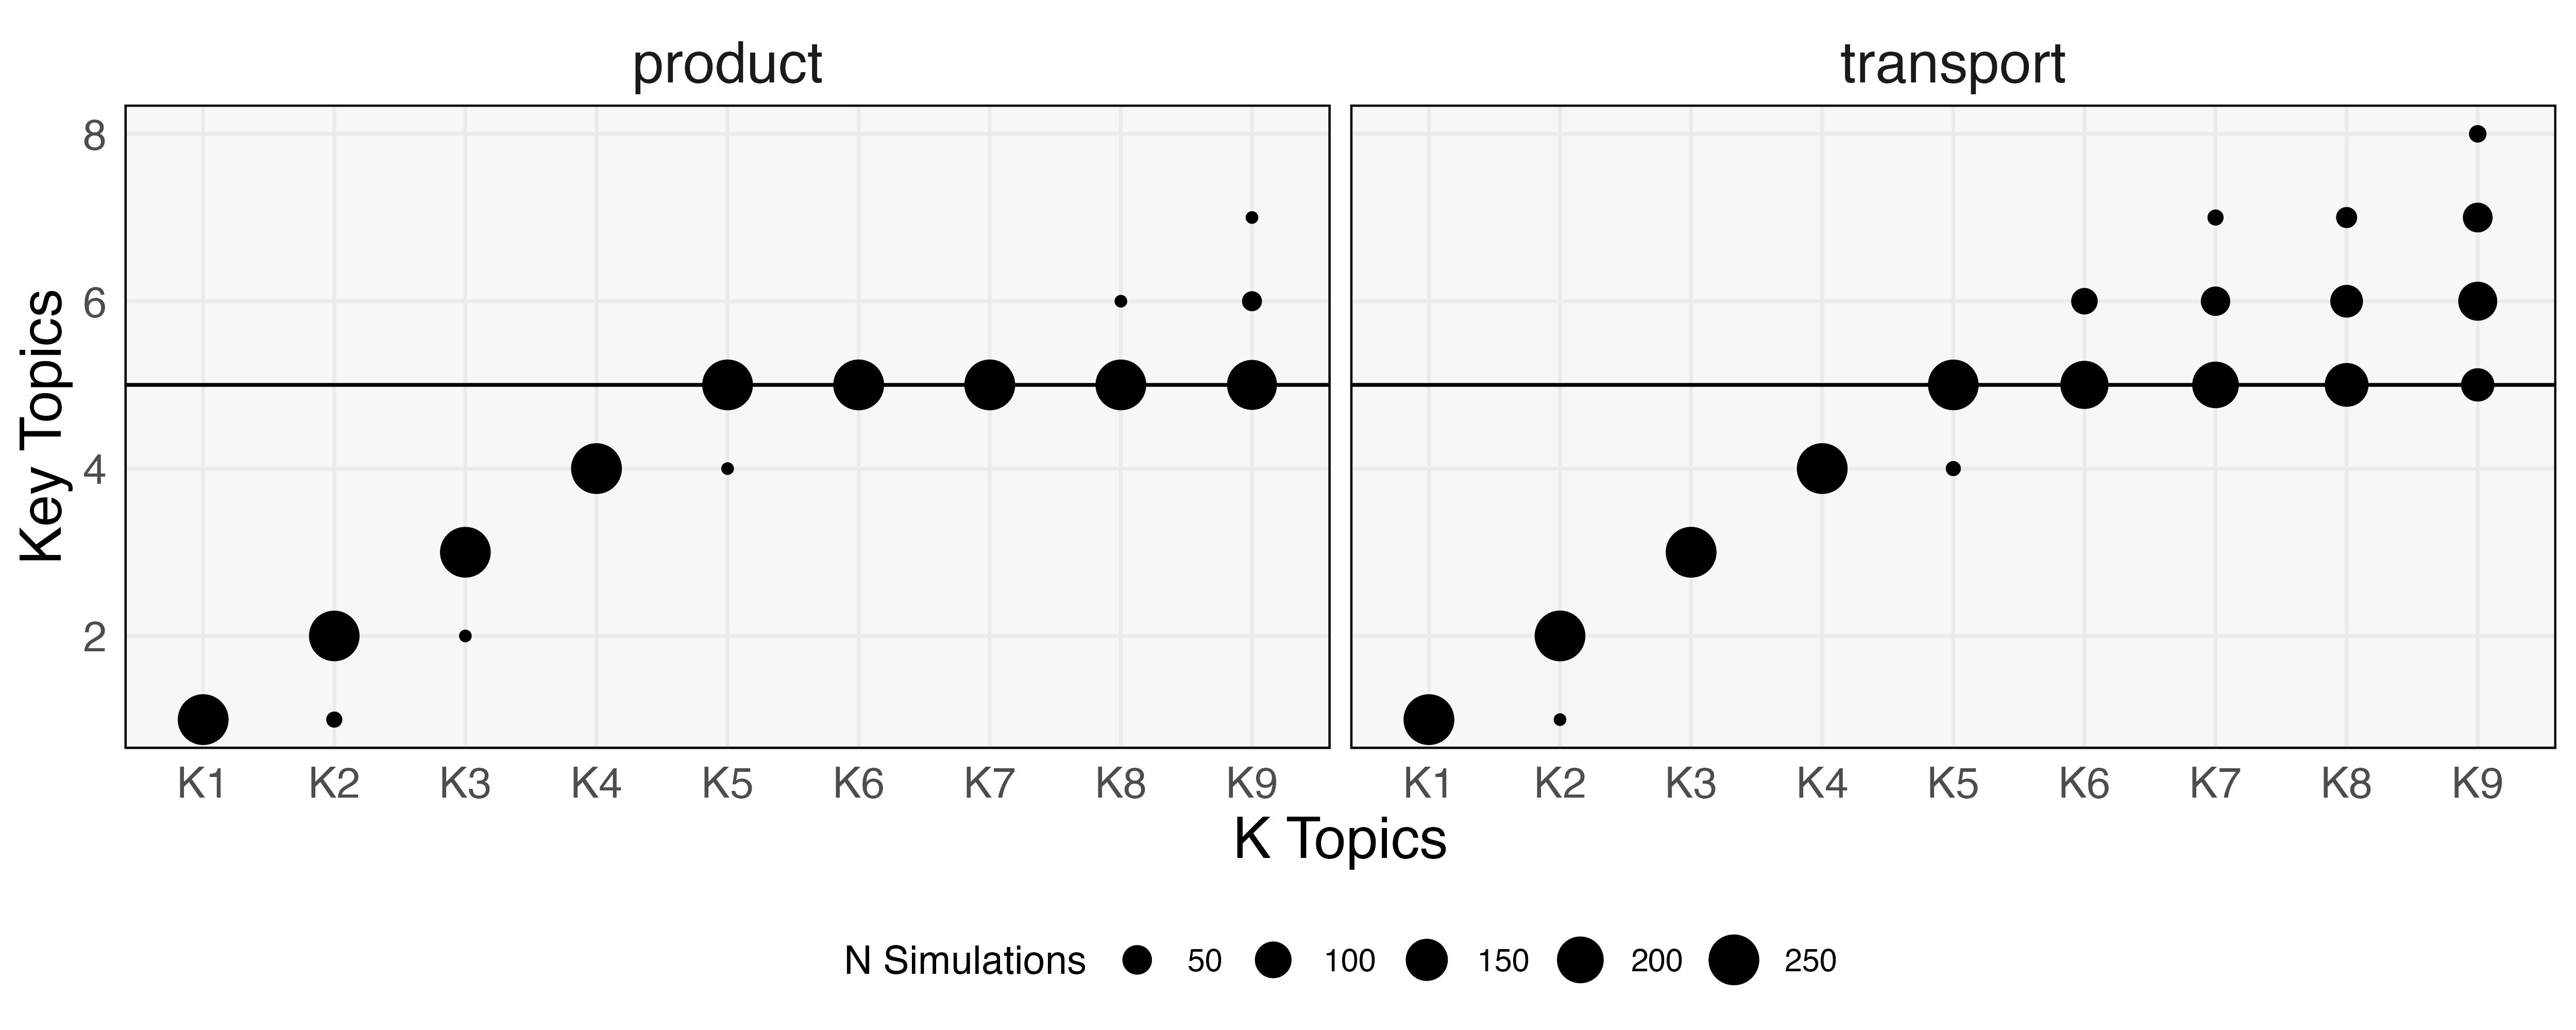
\includegraphics[width=0.65\textwidth]{key_topics-lda}}
    \hfil
    \subfloat{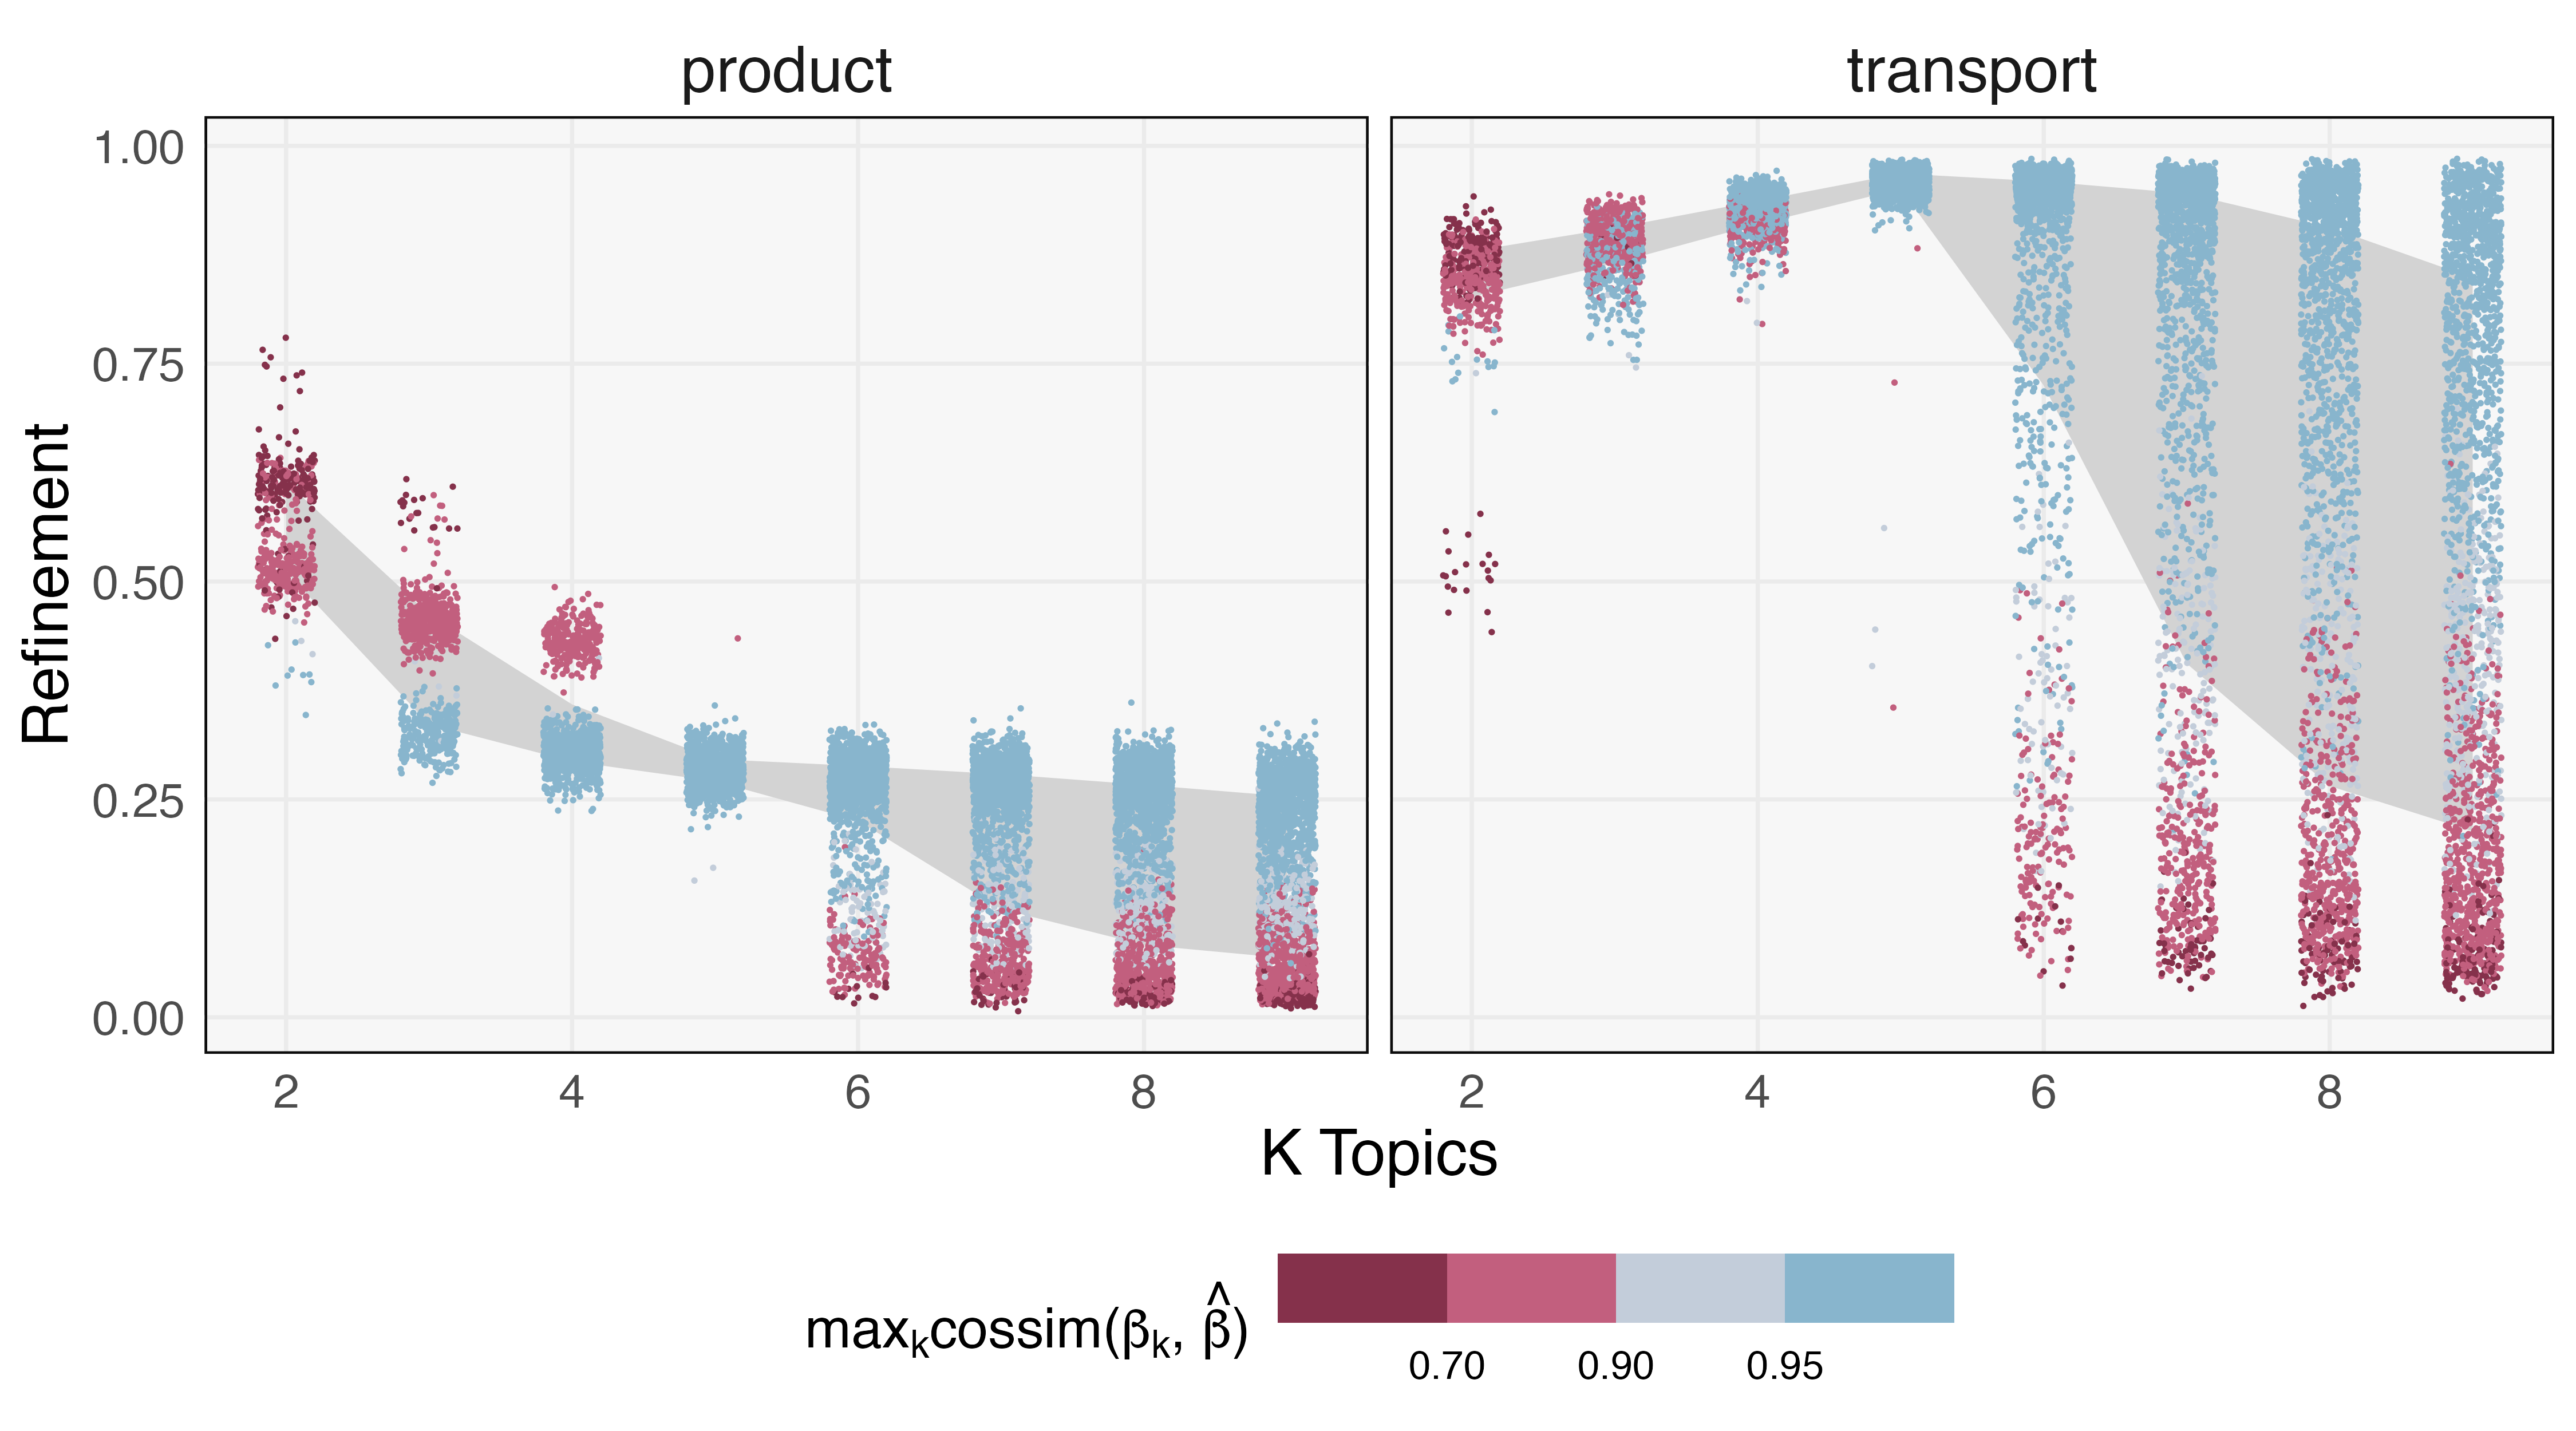
\includegraphics[width=0.65\textwidth]{refinement_lda}}
  \end{figure}
\end{frame}

\begin{frame}
  \frametitle{LDA with background variation}
  What happens when the LDA model is mis-specified? Consider the following
  generative mechanism,
  \begin{align*}
x_{i} \vert \*B, \gamma_{i}, \nu_i &\sim \Mult\left(x_{i} ; N_{i}, \alpha \*B\gamma_{i} + \left(1 - \alpha\right)\nu_i\right) \\
\nu_{i} &\sim \Dir\left(\lambda_{\nu}\right) \\
\gamma_i &\sim \Dir\left(\lambda_{\gamma}\right) \\
\beta_{k} &\sim \Dir\left(\lambda_{\beta}\right),
\end{align*}
where $\*B$ stacks the $\beta_k$ rowwise.
\end{frame}

\begin{frame}
  \frametitle{Result}
  The alignment structure is sensitive to changes in $\alpha$ and fragments when
  LDA structure is not present.

\begin{figure}
    \subfloat{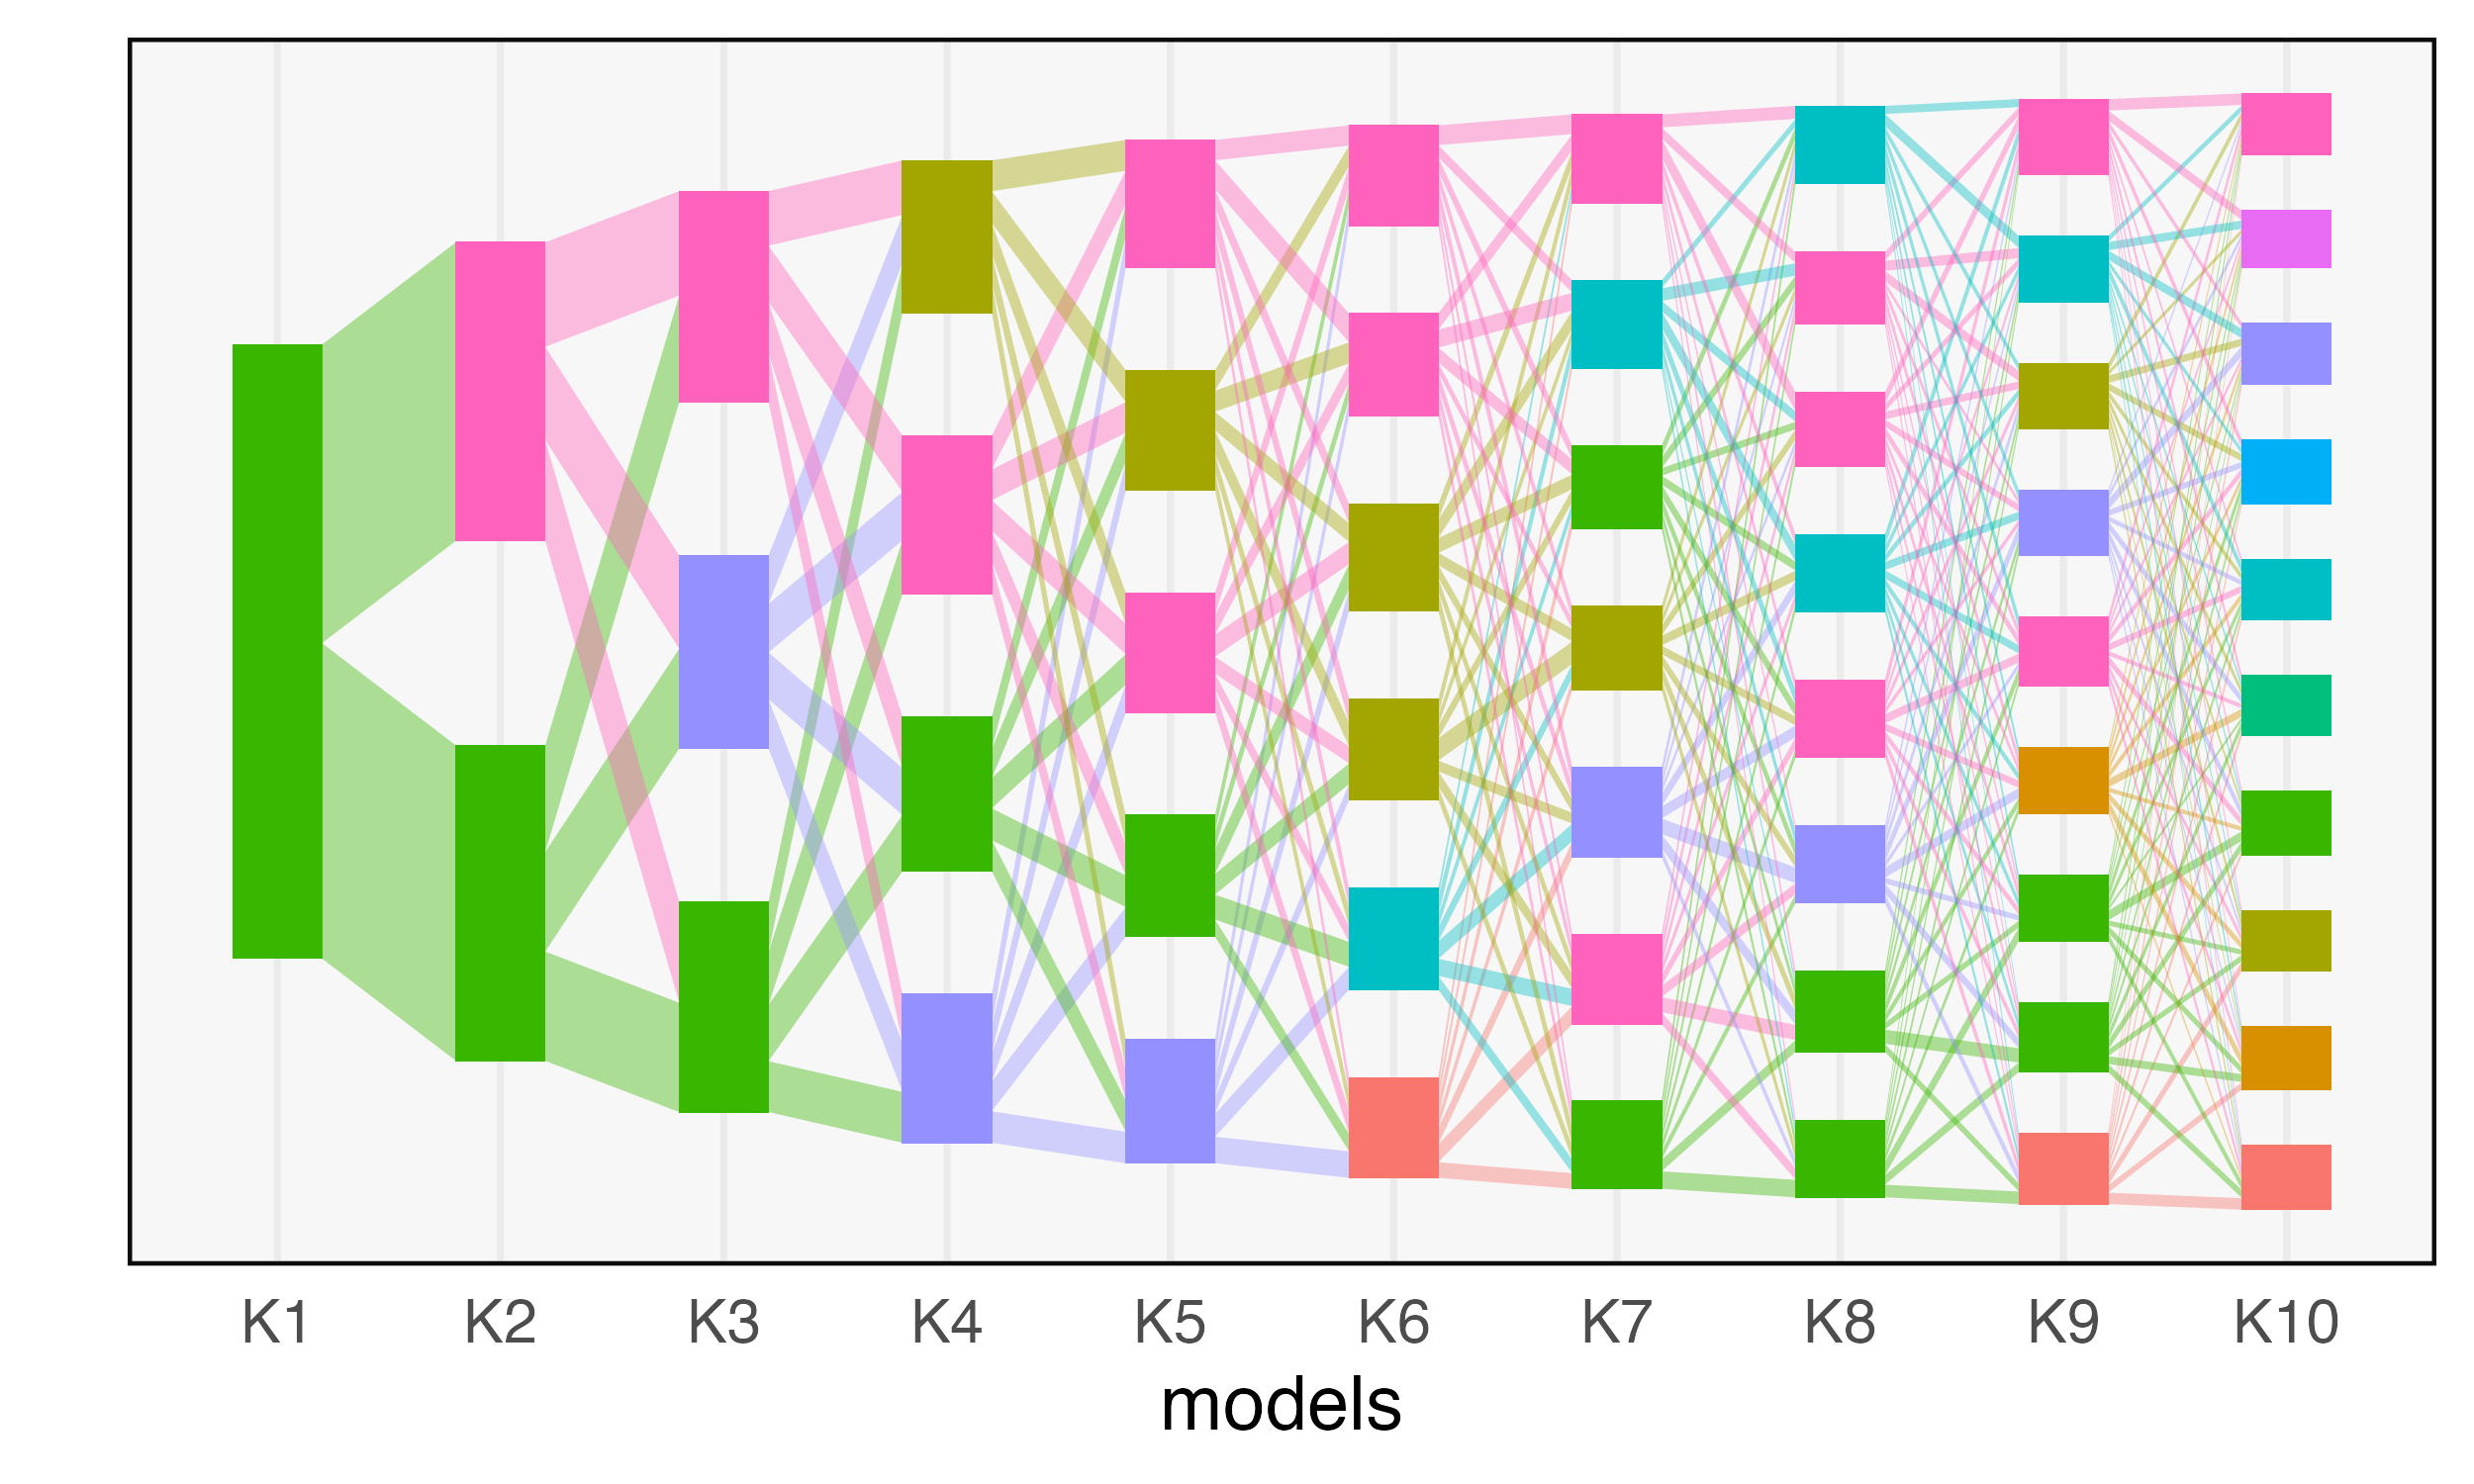
\includegraphics[width=0.4\textwidth]{gradient_flow-1}}
    \subfloat{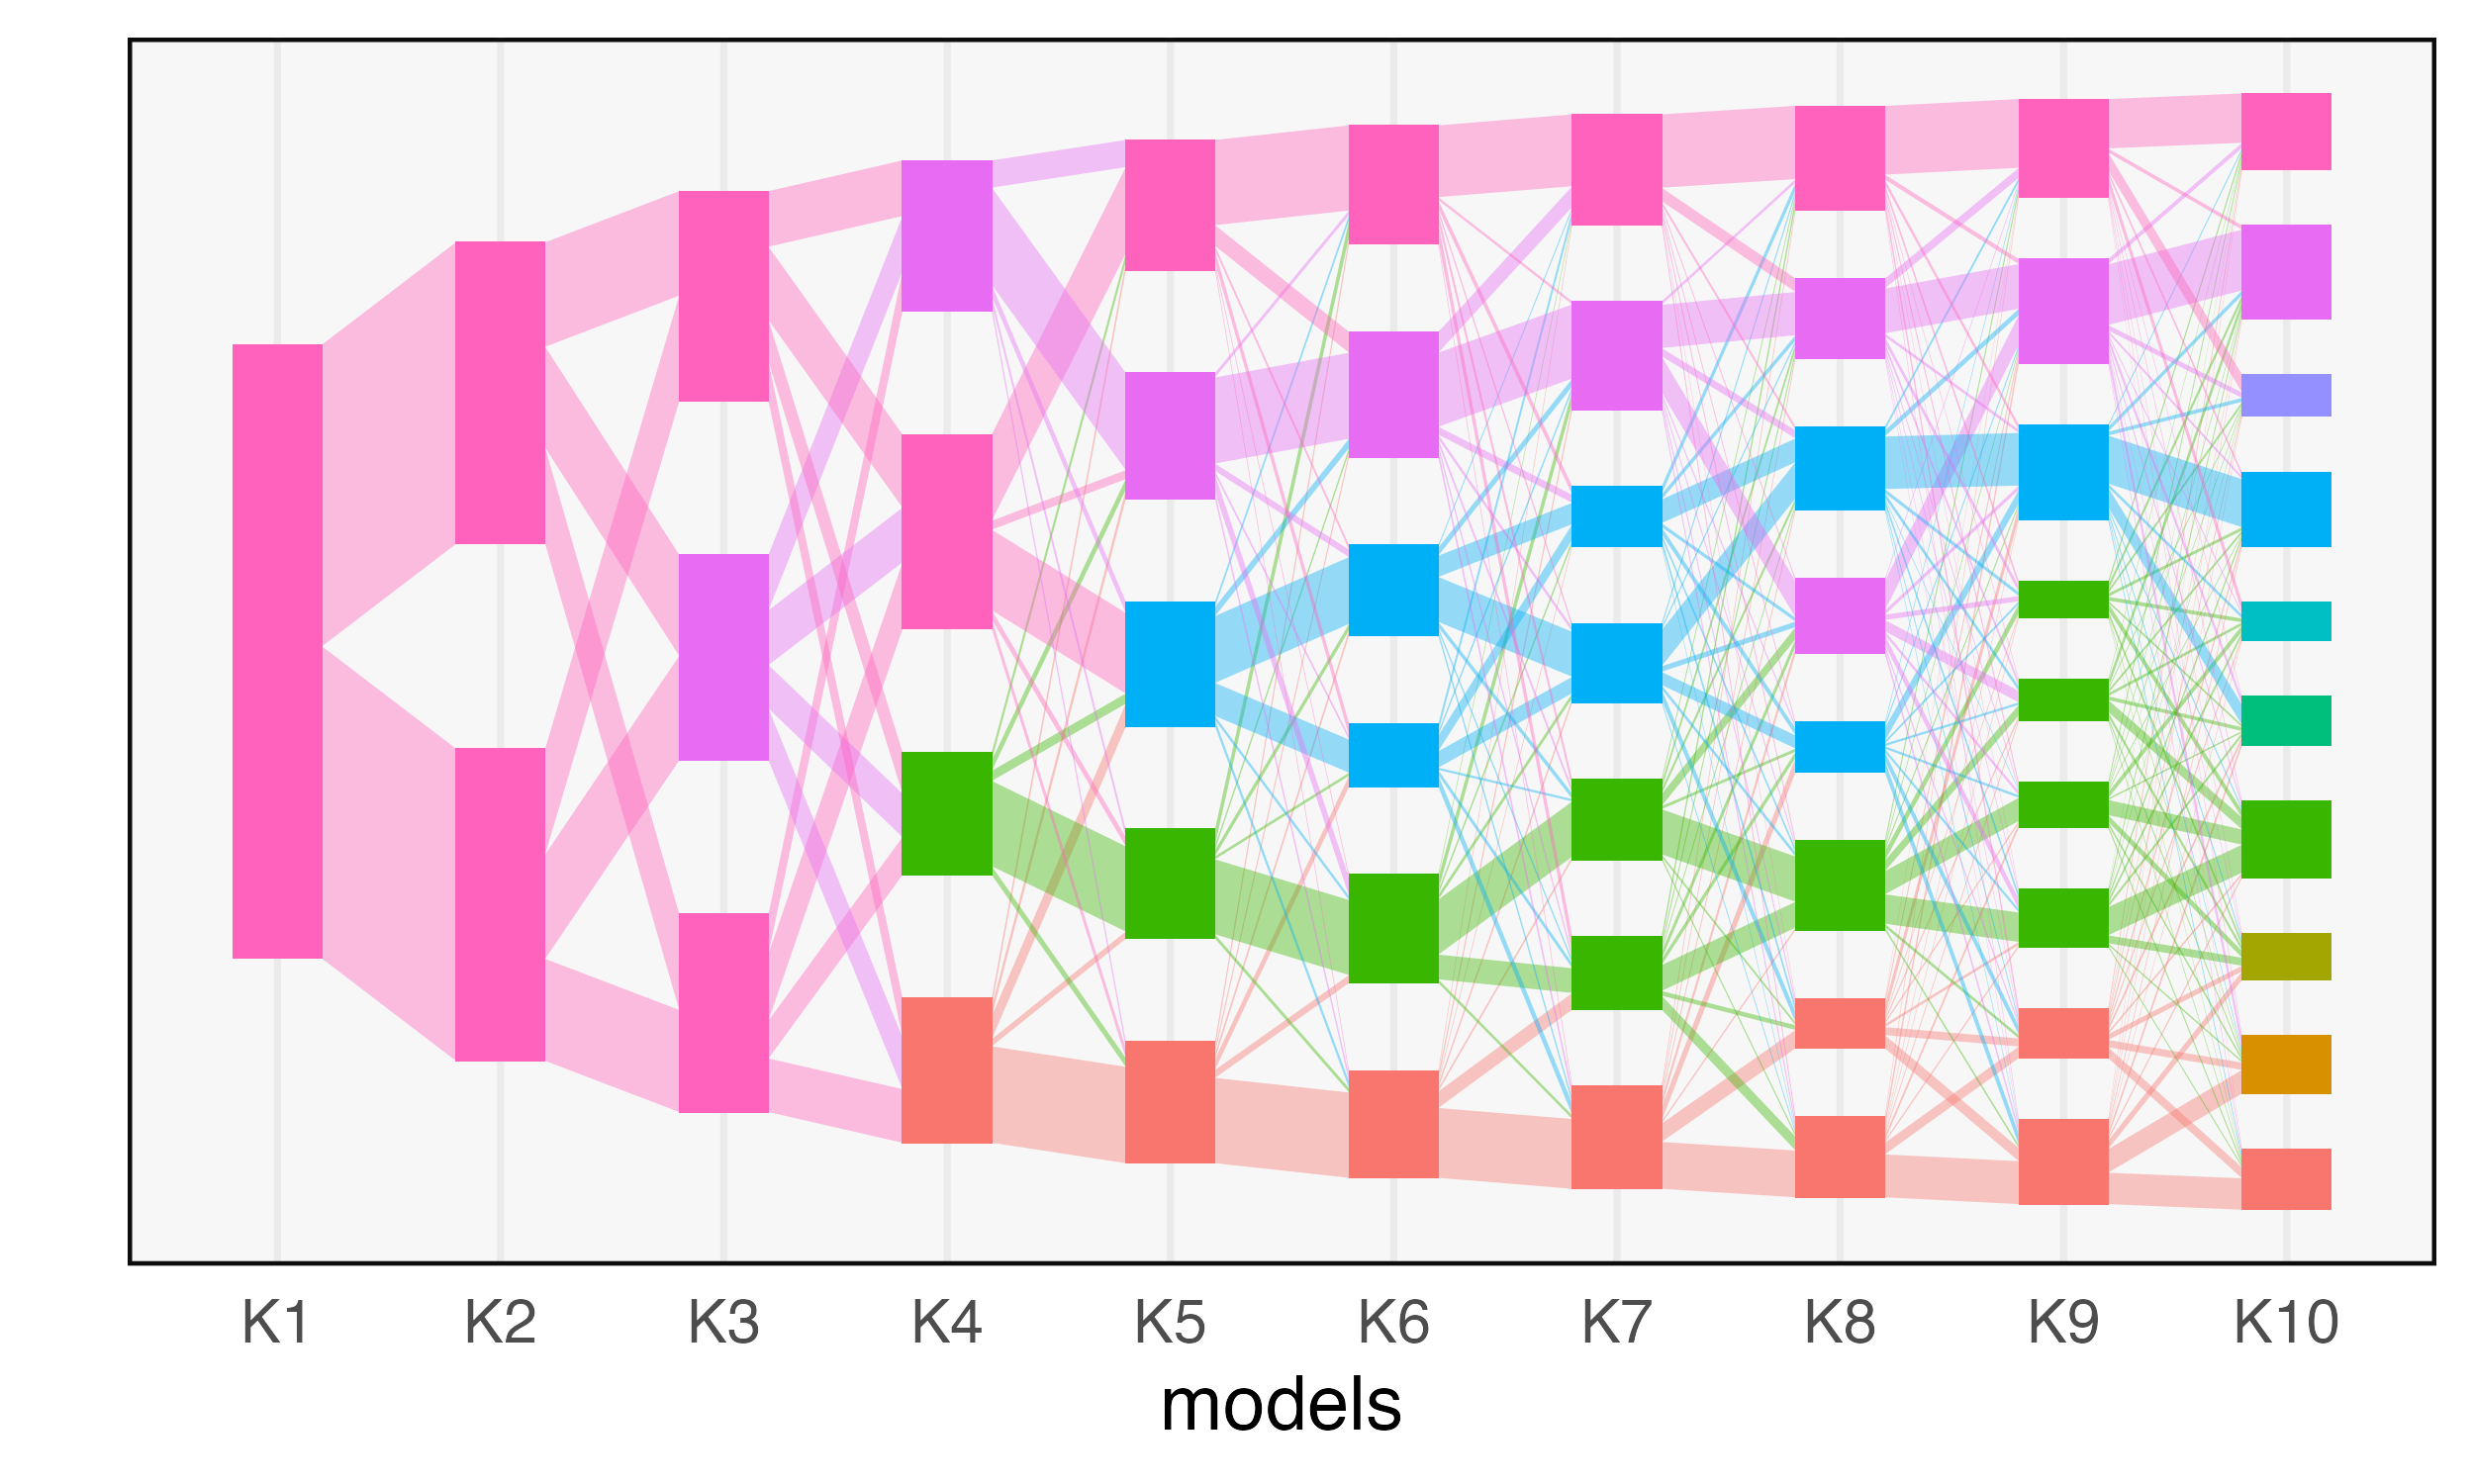
\includegraphics[width=0.4\textwidth]{gradient_flow-2}}
    \hfil
    \subfloat{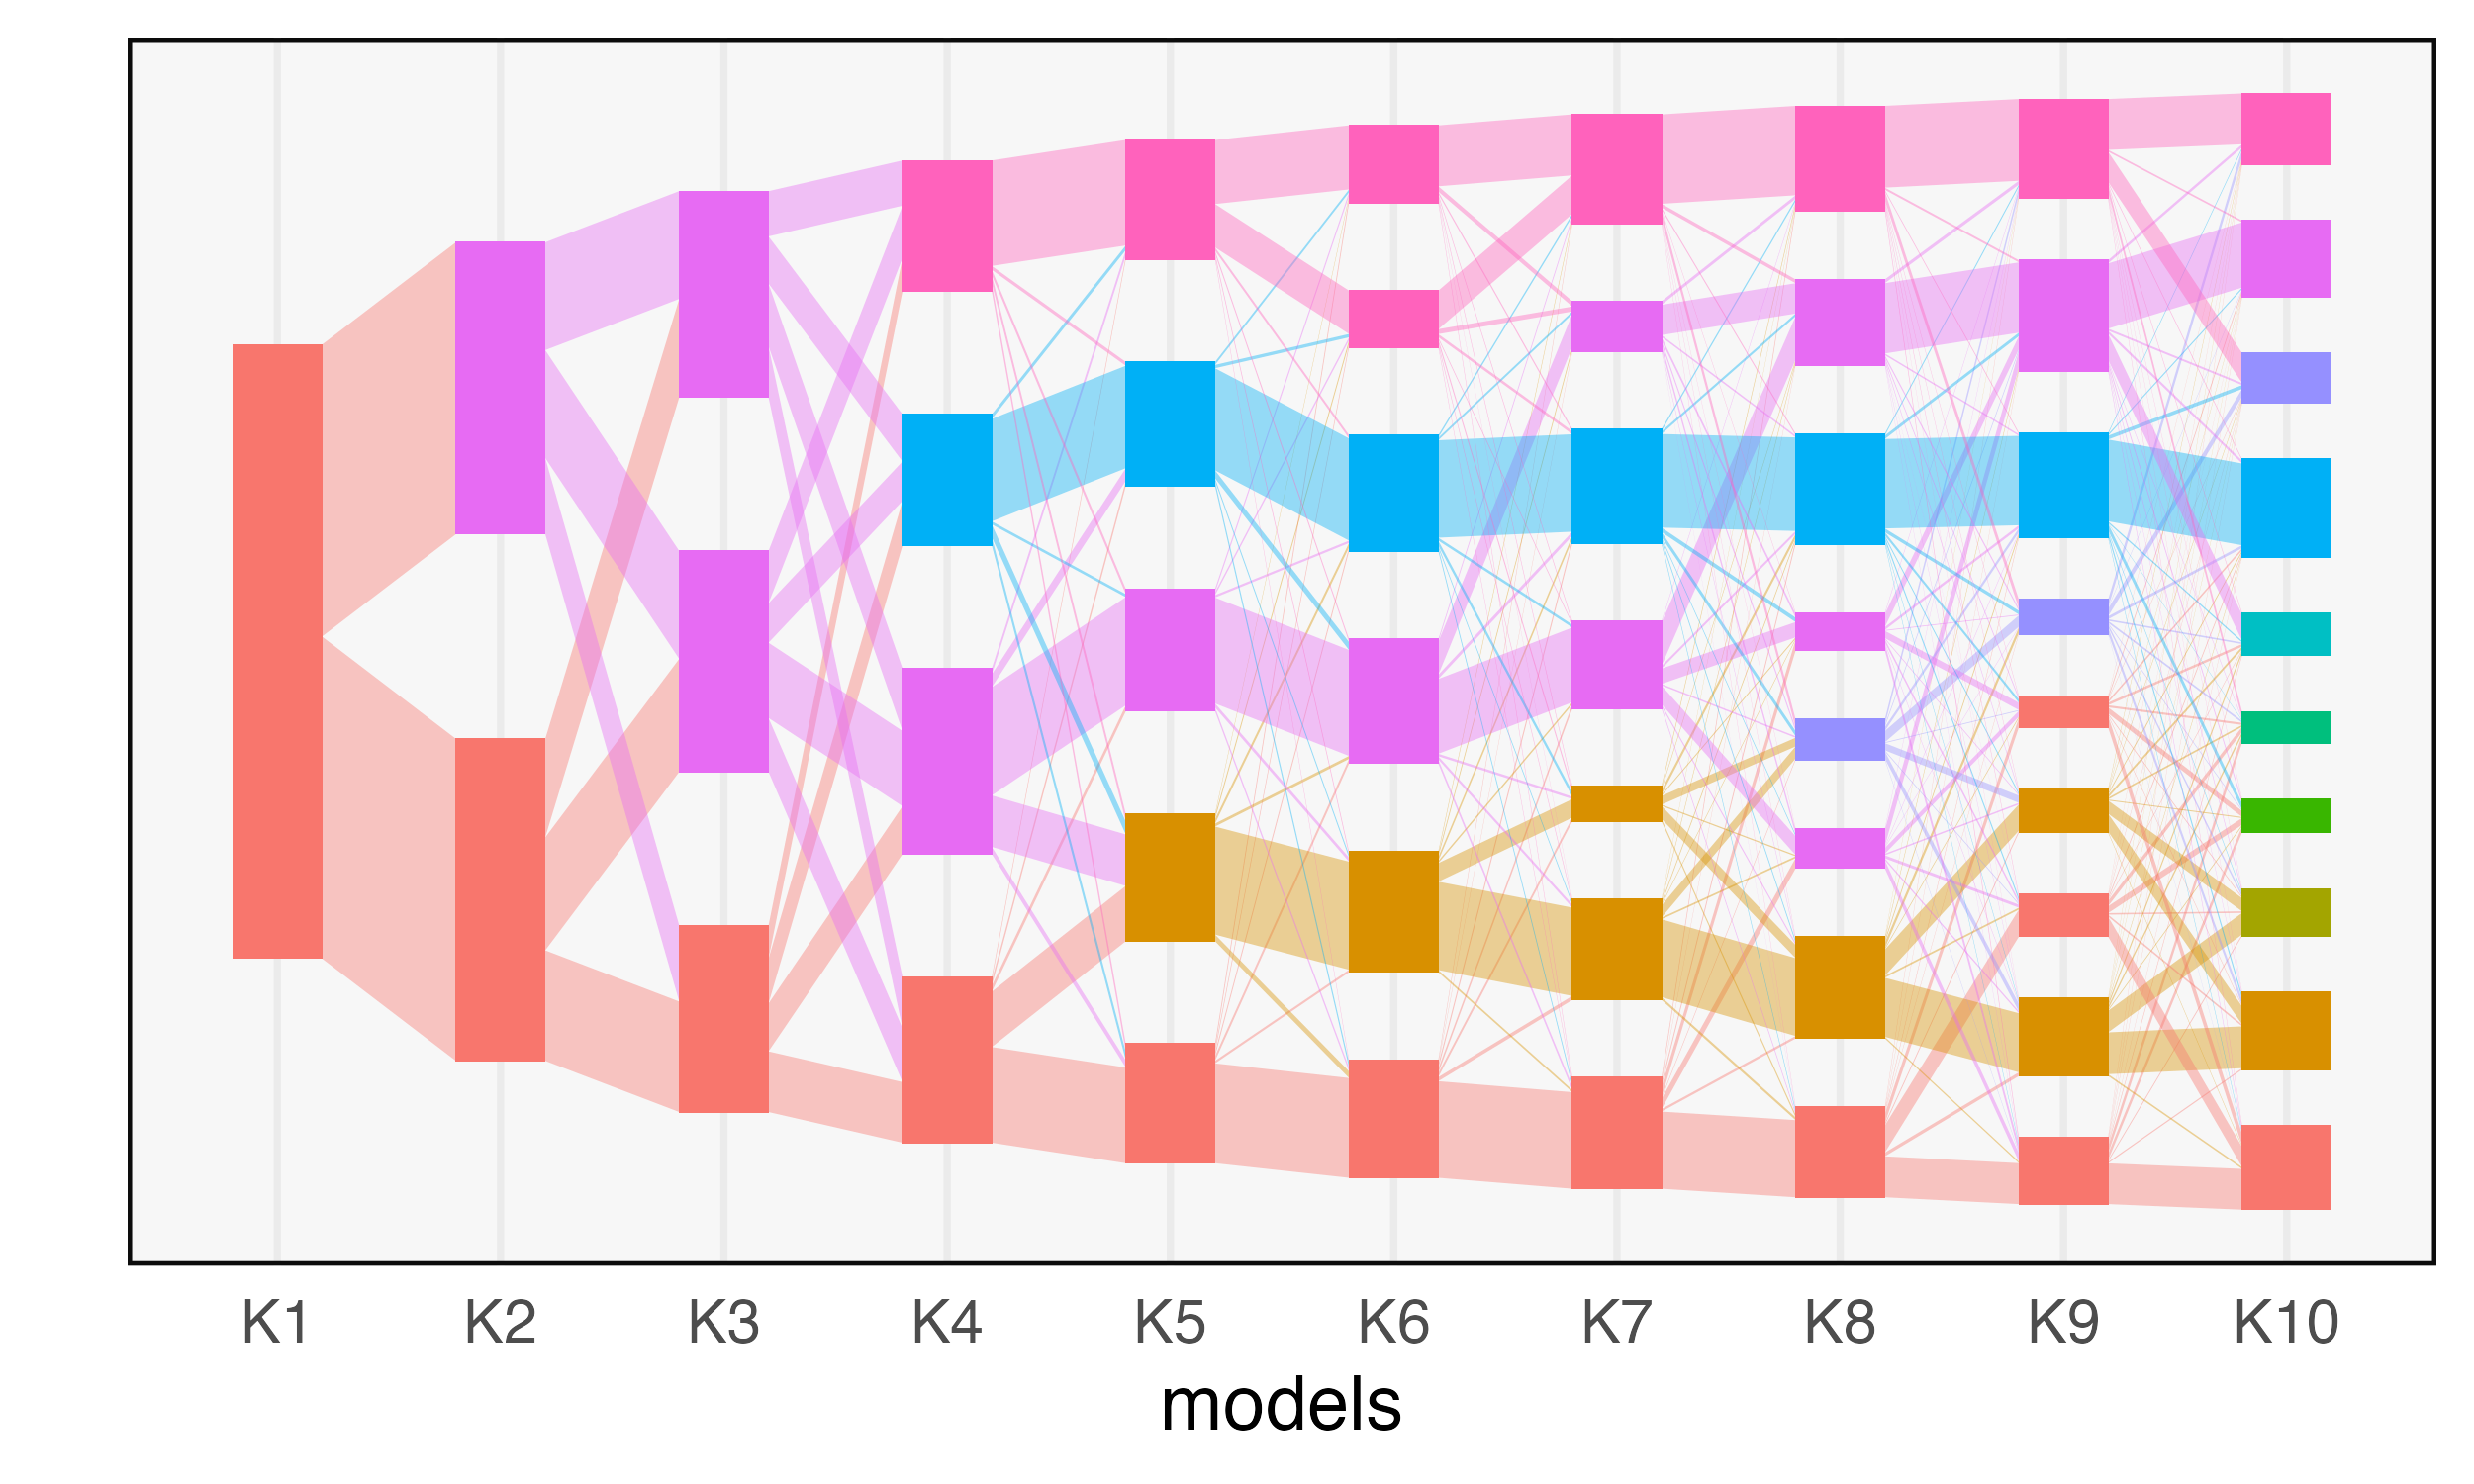
\includegraphics[width=0.4\textwidth]{gradient_flow-3}}
    \subfloat{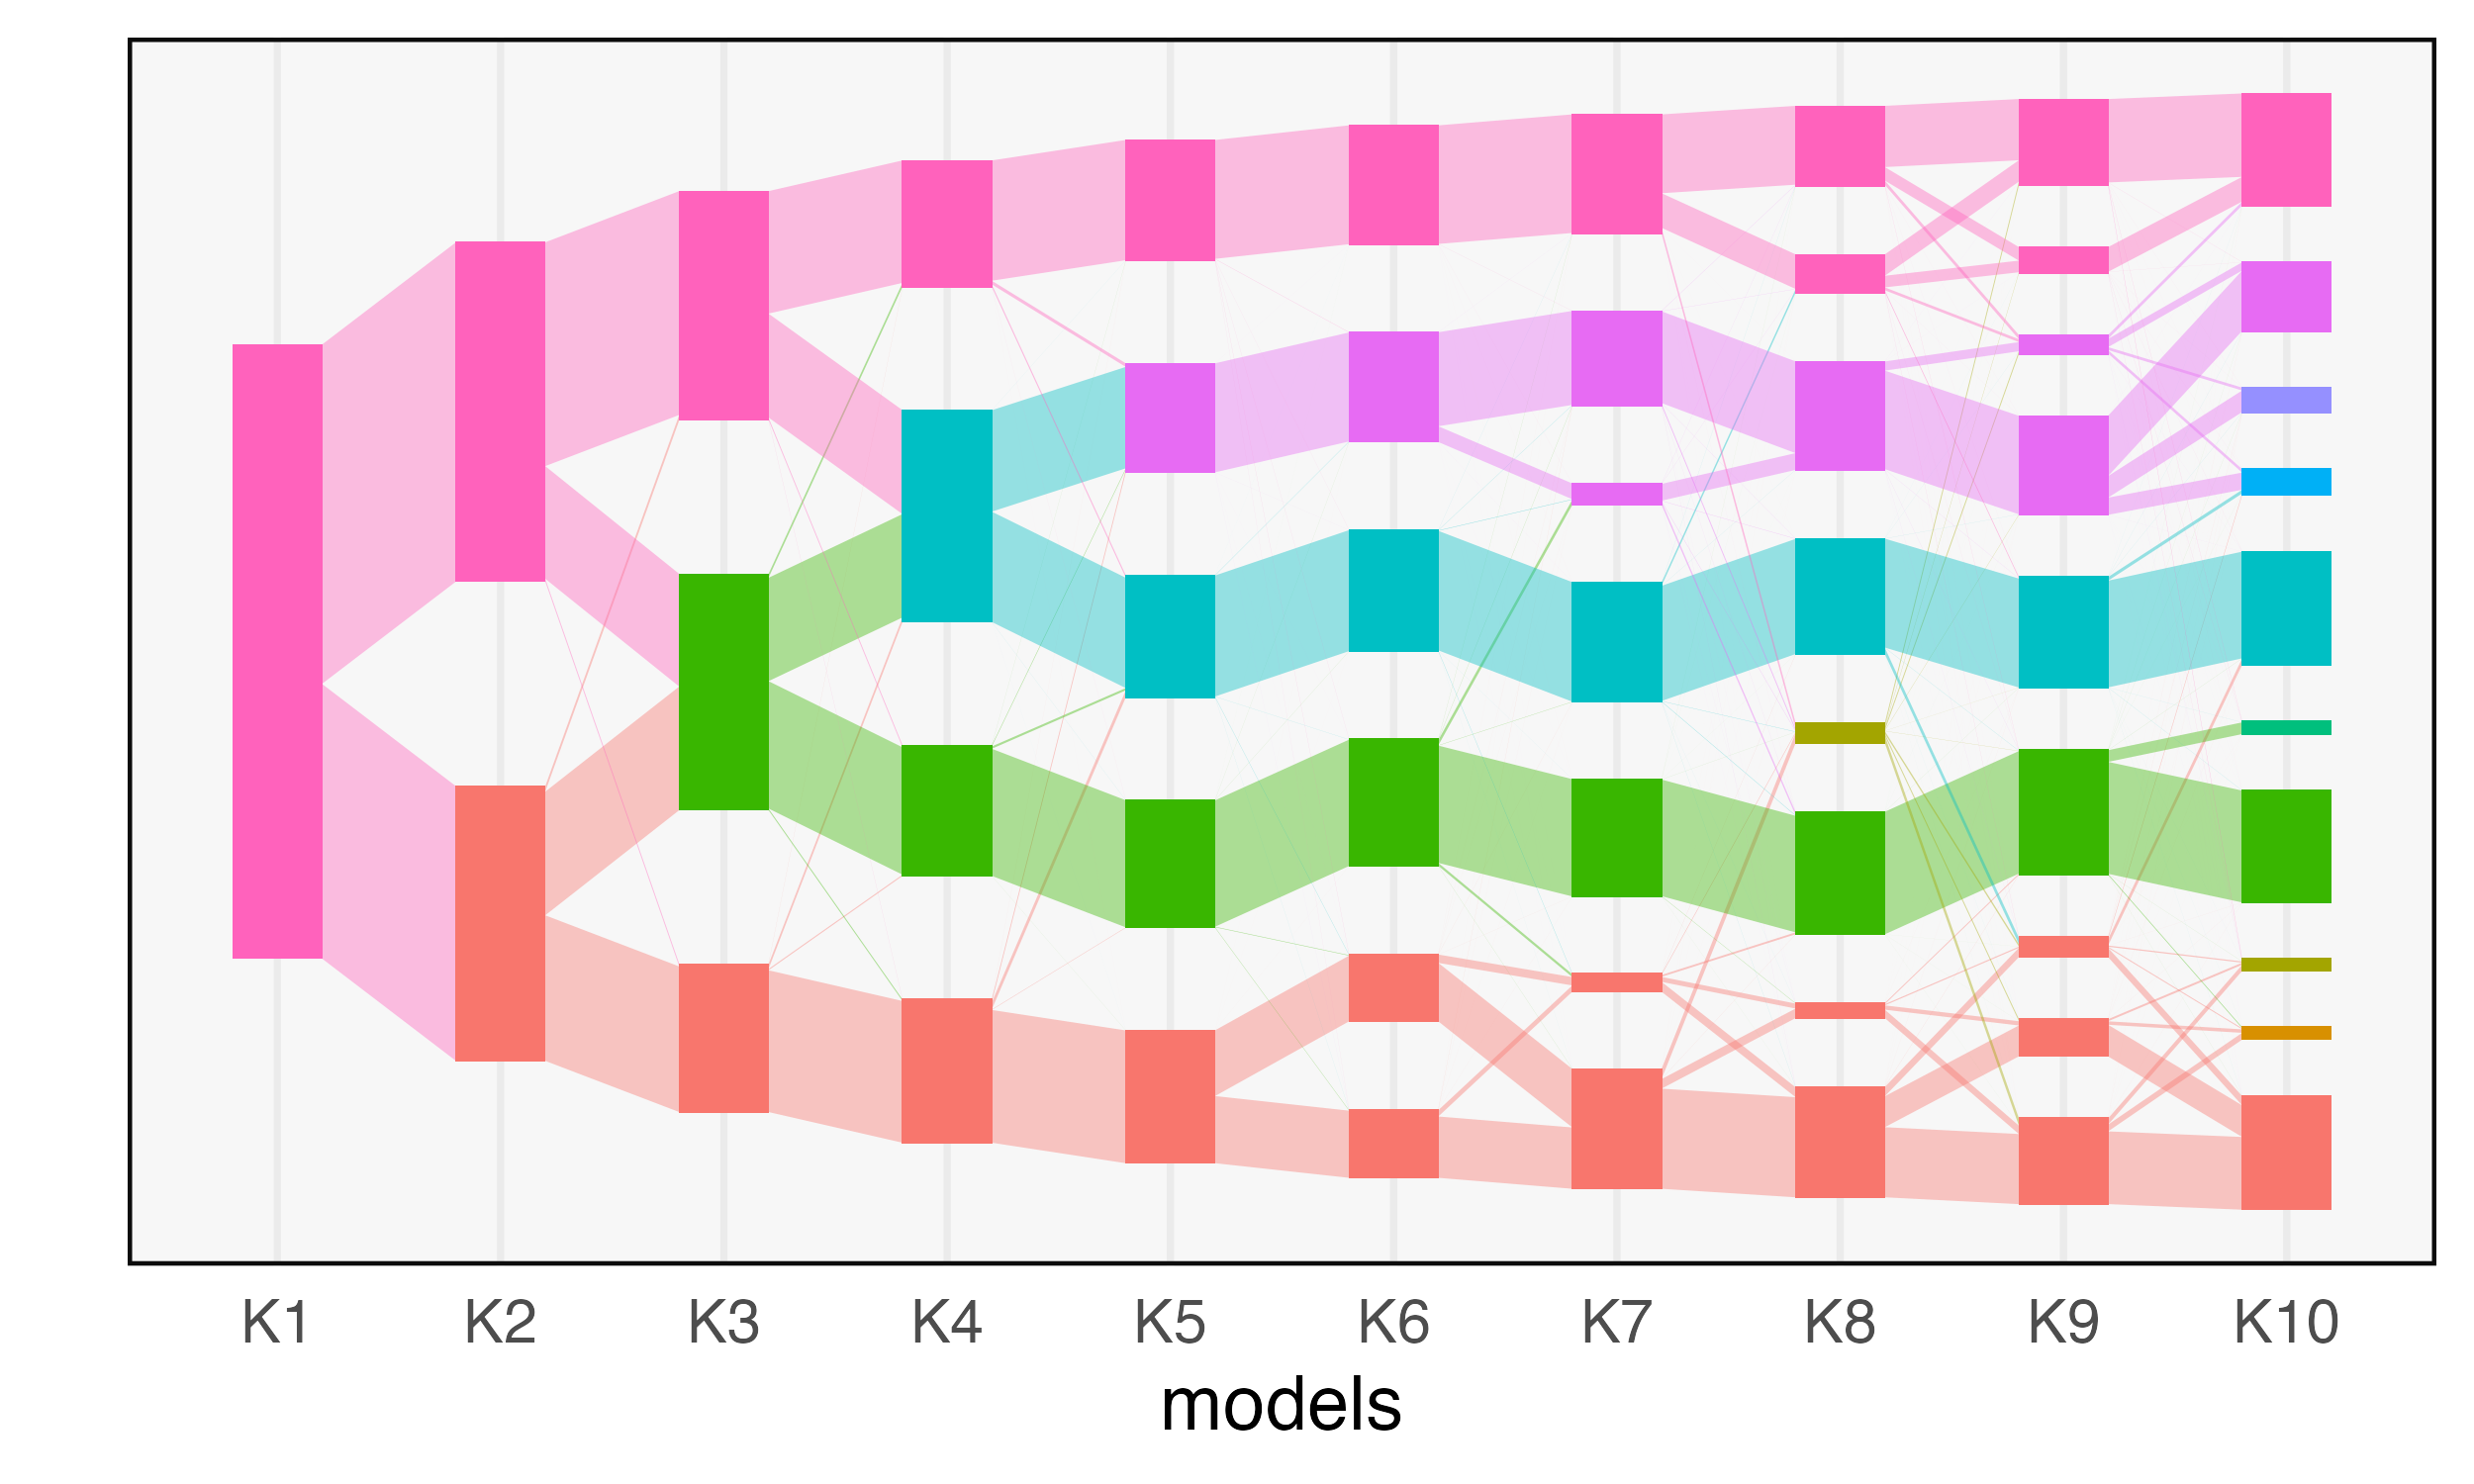
\includegraphics[width=0.4\textwidth]{gradient_flow-4}}
\end{figure}

\end{frame}

\begin{frame}
  \frametitle{Summaries}
  This structure is consistent across simulation runs, and the summary measures
  quantify the deterioration of topics.
\begin{figure}
    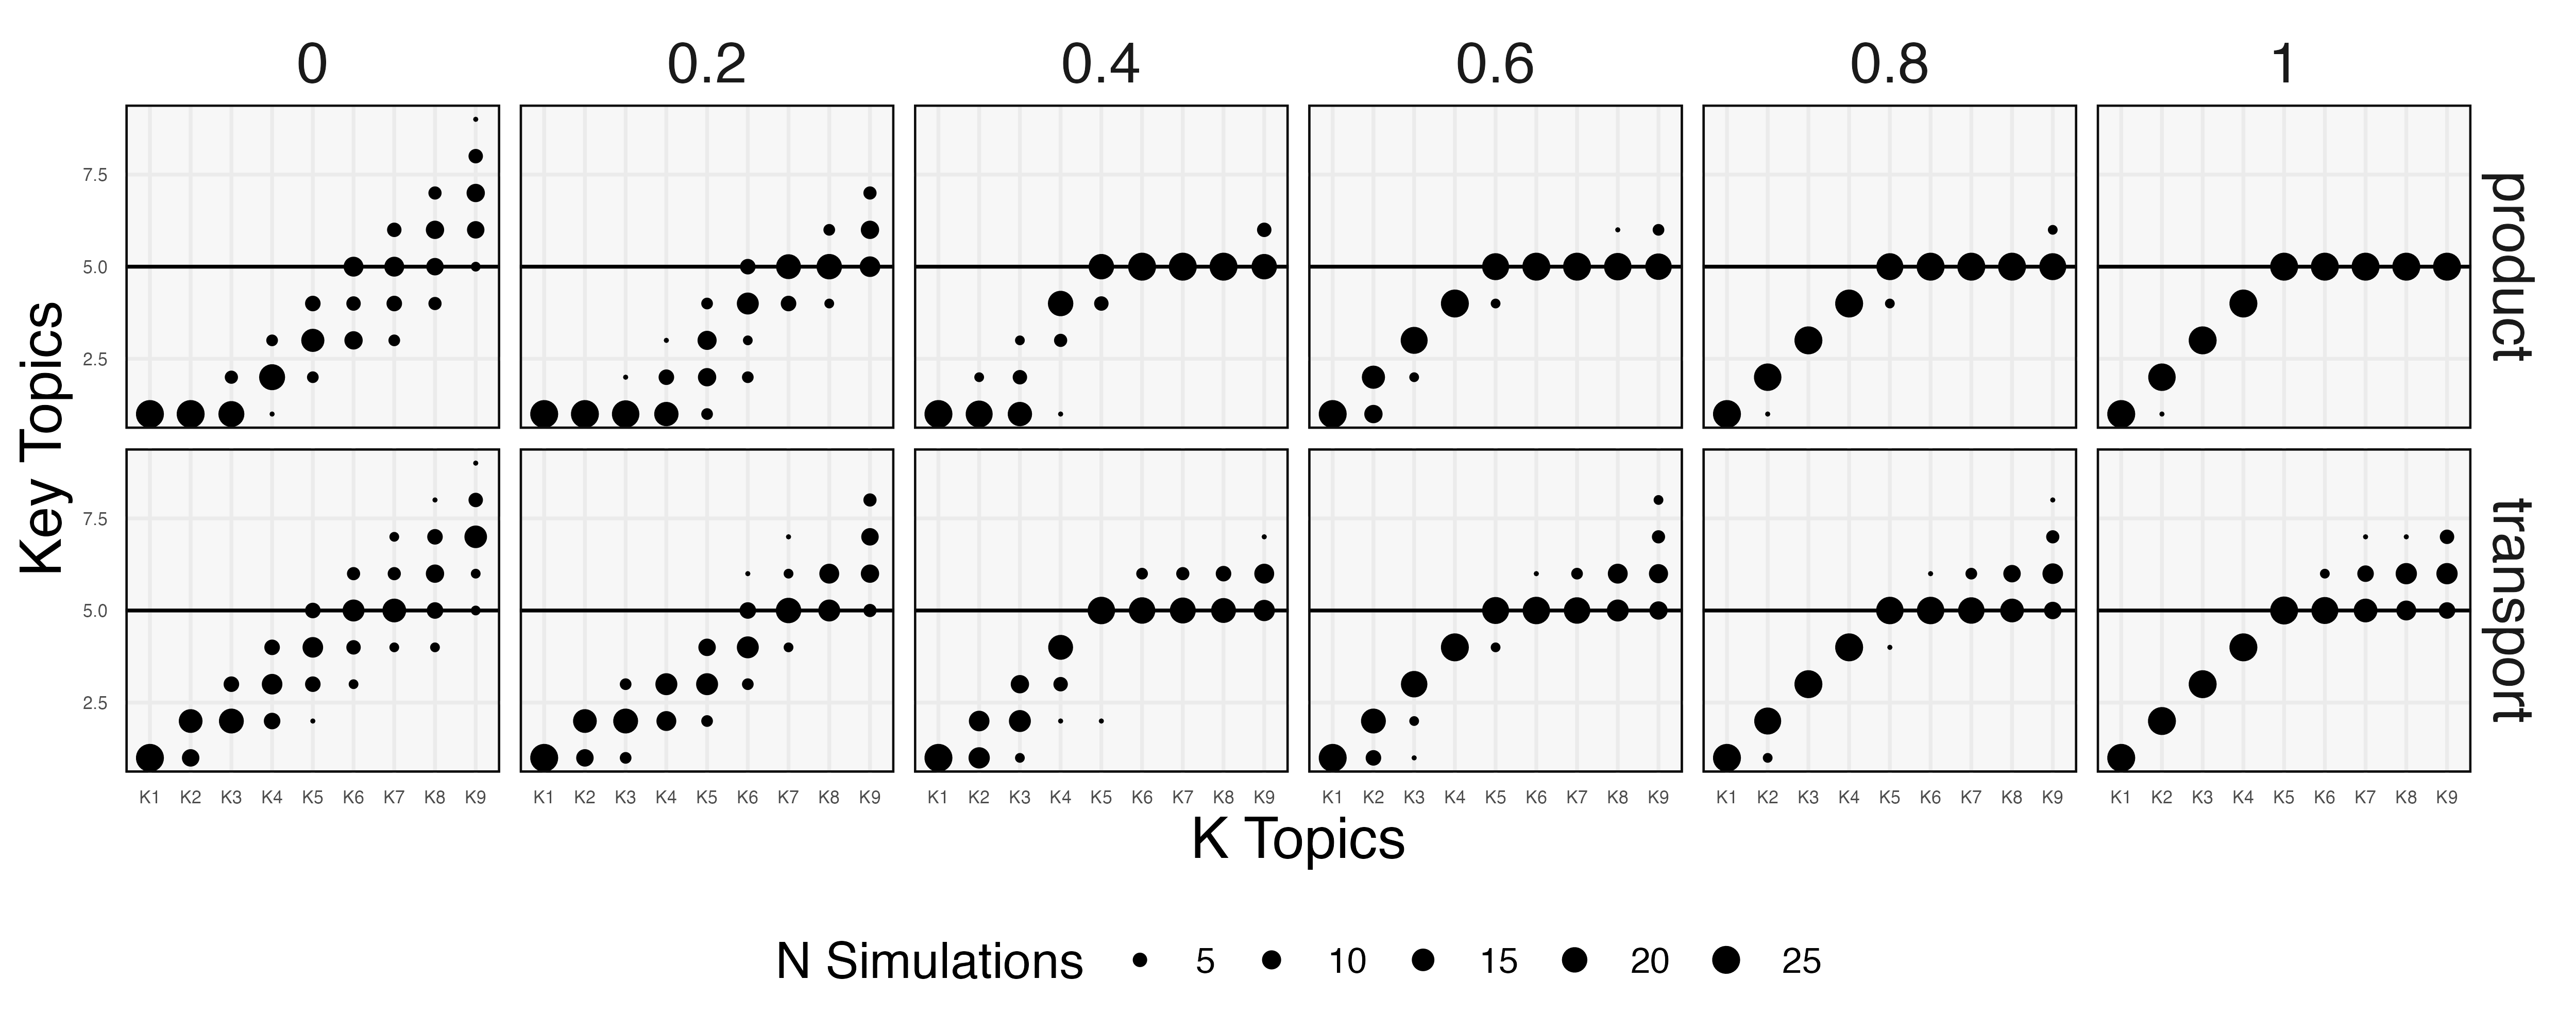
\includegraphics[width=\textwidth]{gradient_key_topics}
\end{figure}
\end{frame}

\begin{frame}
  \frametitle{Summaries}
  This structure is consistent across simulation runs, and the summary measures
  quantify the deterioration of topics.
\begin{figure}
    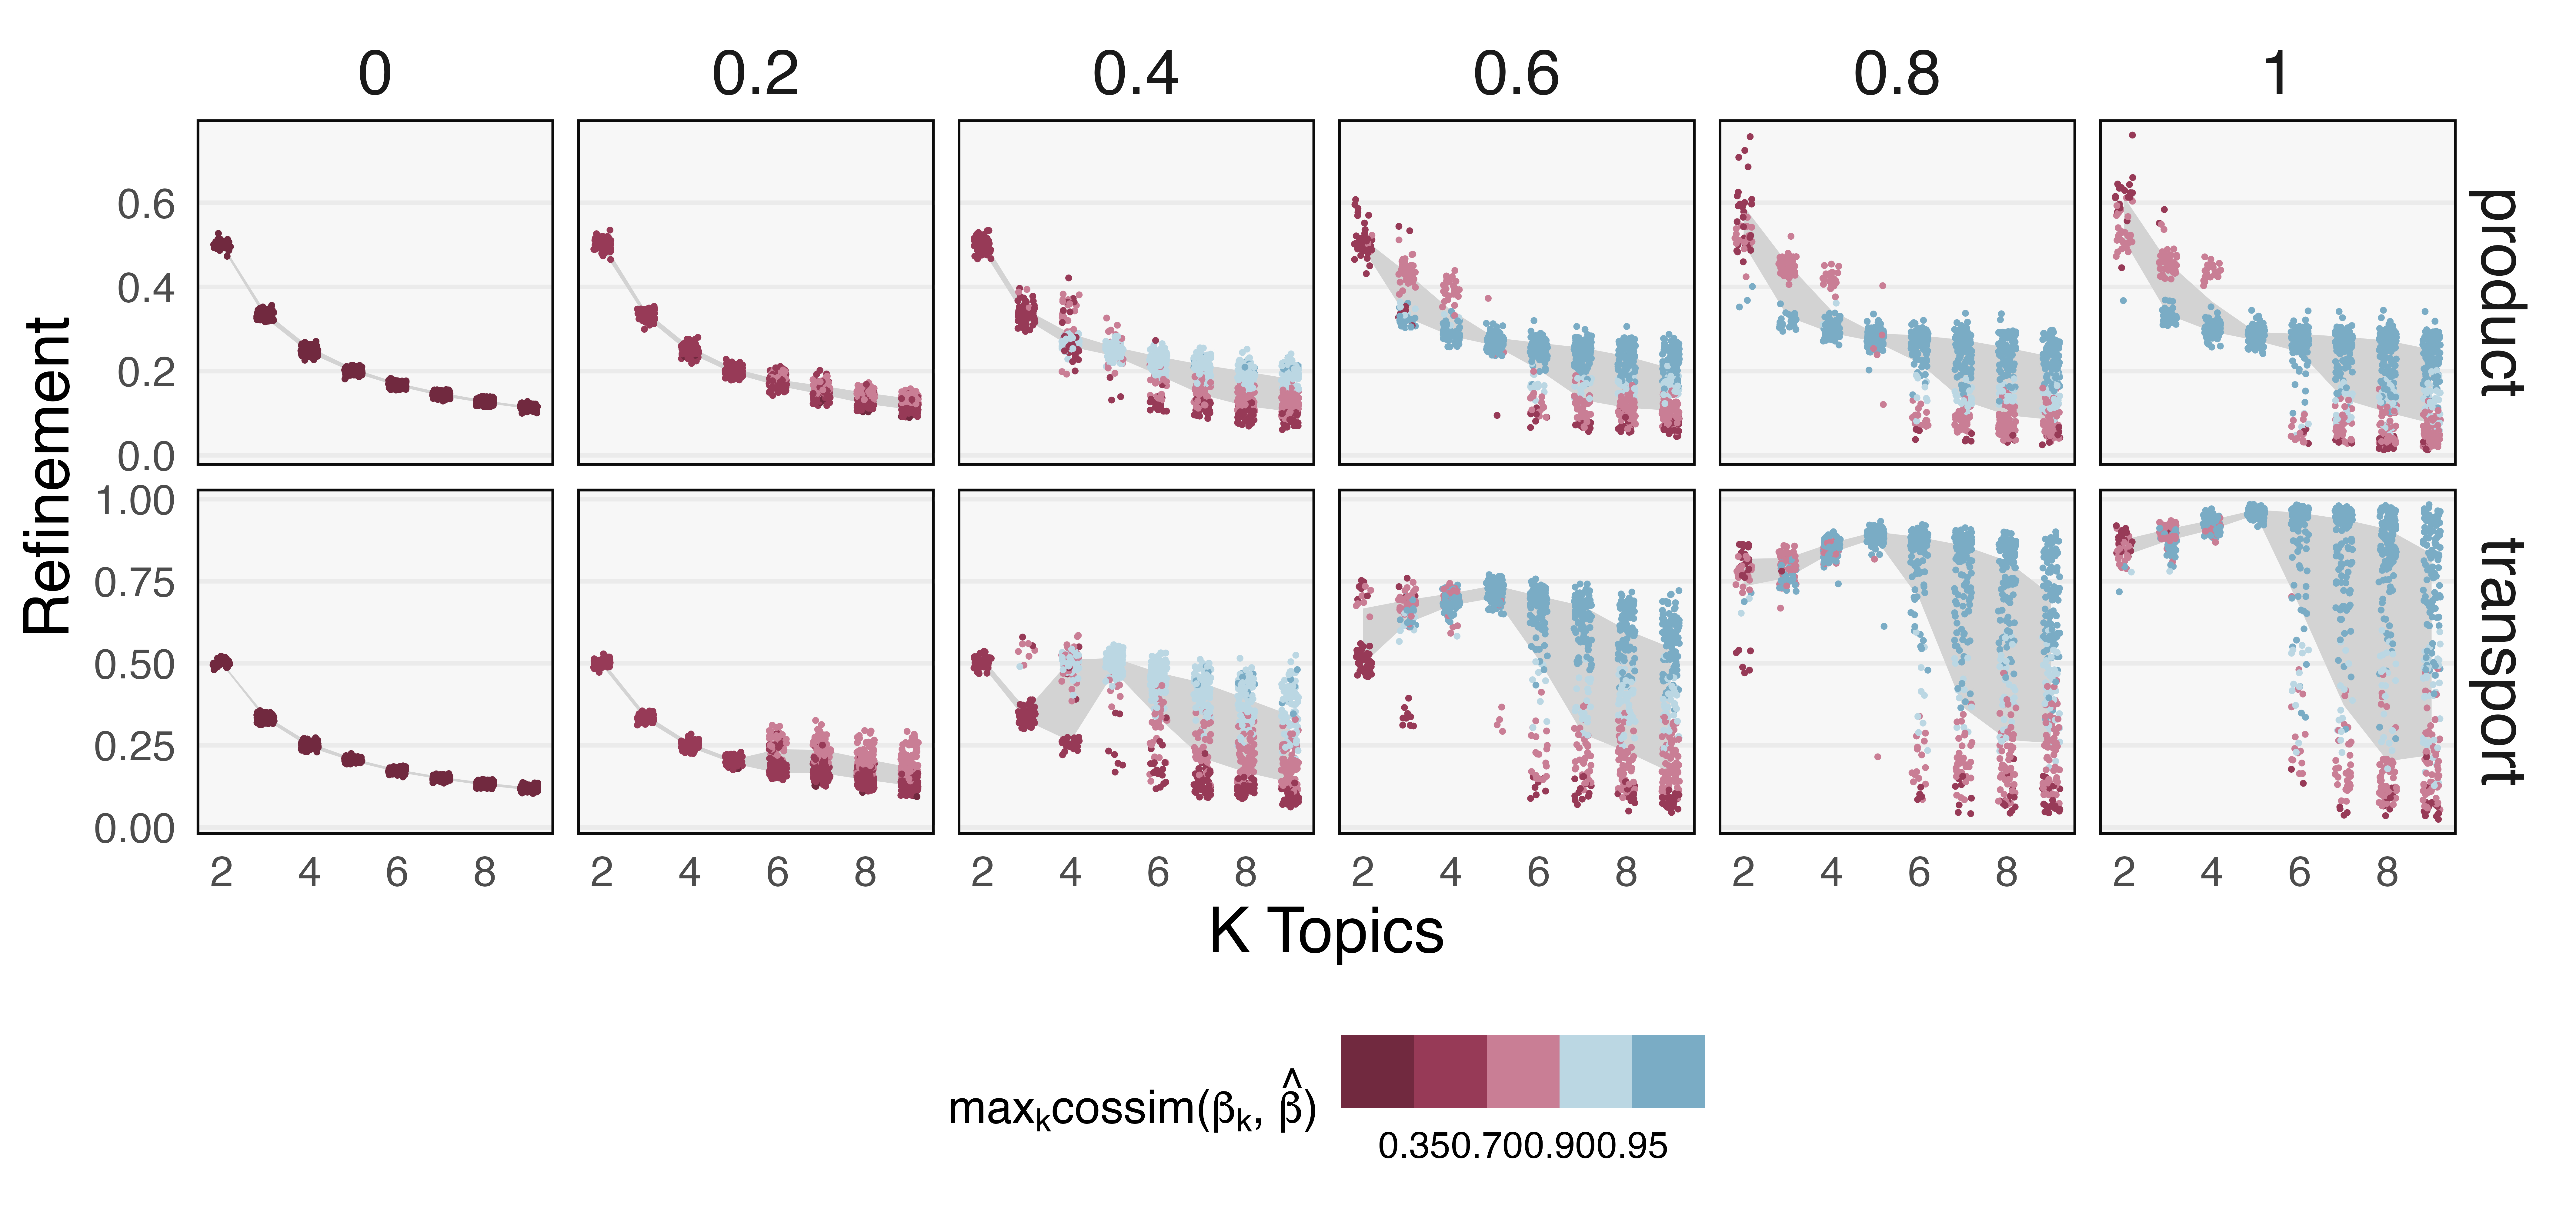
\includegraphics[width=\textwidth]{gradient_refinement_full}
\end{figure}
\end{frame}

\begin{frame}
  \frametitle{Summaries}
  This structure is consistent across simulation runs, and the summary measures
  quantify the deterioration of topics.
\begin{figure}
    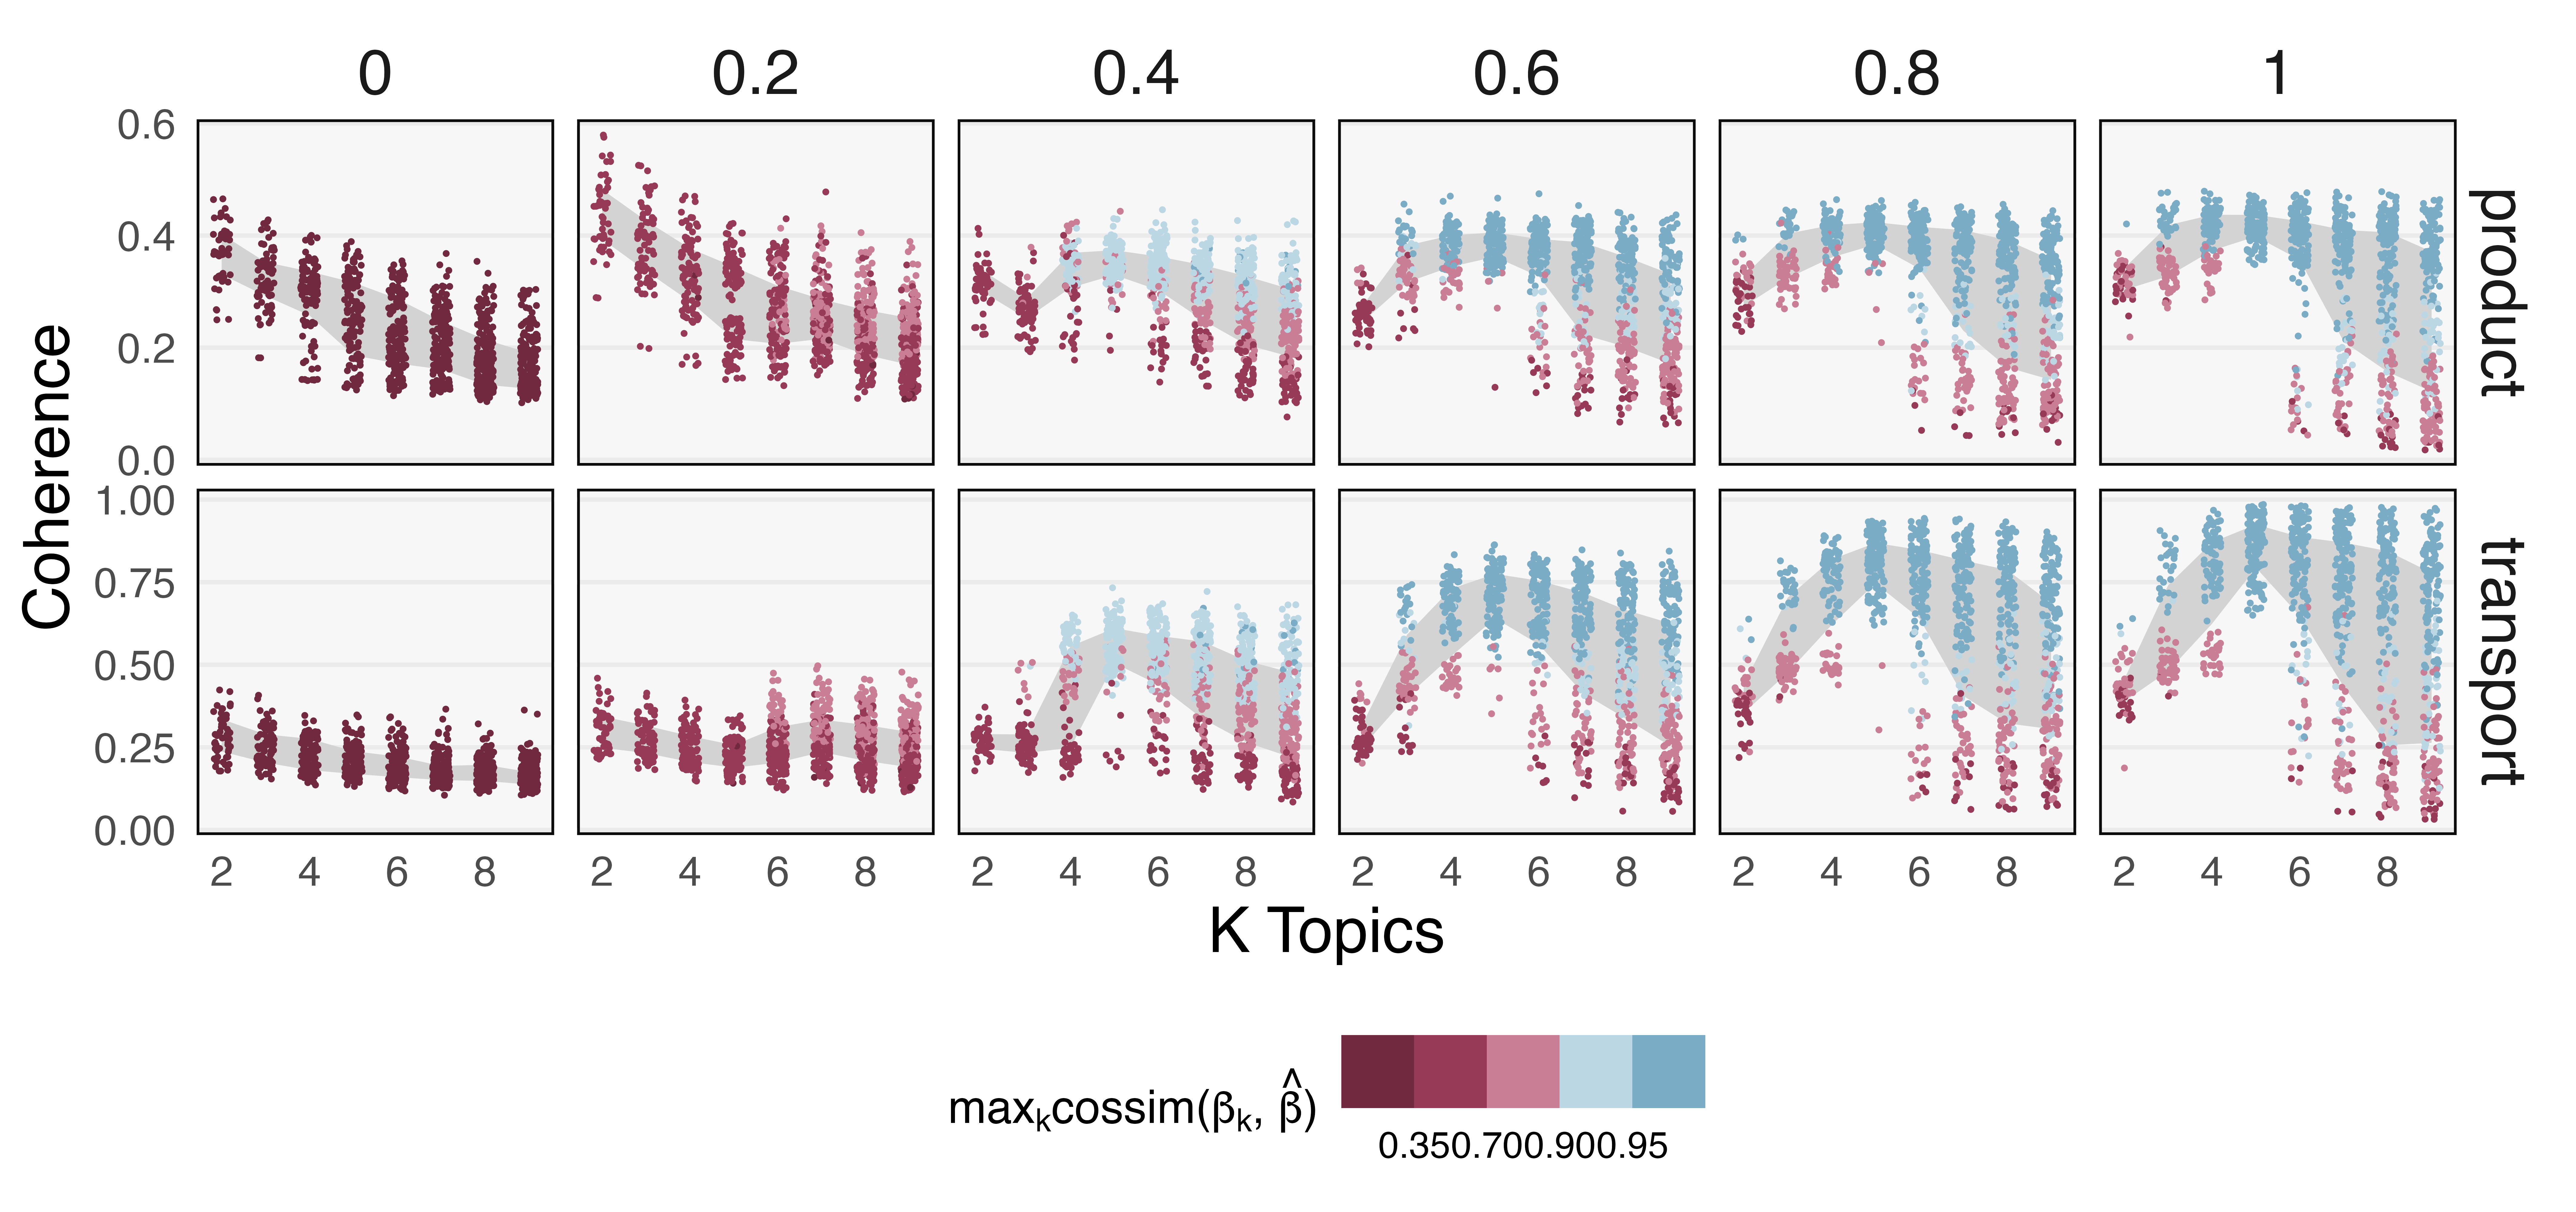
\includegraphics[width=\textwidth]{gradient_stability}
\end{figure}
\end{frame}

\begin{frame}
  \frametitle{Strain switching}
  Our final simulation mimics the strain switching problem.
  \begin{itemize}
    \item Small subsets of species switch between two otherwise similar topics
    \item Multiple resolutions are required to detect the difference
  \end{itemize}
\end{frame}

\begin{frame}
\frametitle{Mechanism}
We first construct equivalence classes of similar topics $\tilde{\beta}_k^r$.
Then, for each sample $i$ and each $k$, we draw one member from the class
\begin{align*}
\beta_{k}^{i} &\sim \Unif\left(\left\{\tilde{\beta}_{k}^{1}, \dots, \tilde{\beta}_{k}^{R}\right\}\right)
\end{align*}
stack the results into $B^{i}$, and then draw,
\begin{align}
x_{i} &\sim \Mult\left(n_{i}, B^{i}\gamma_{i}\right)
\end{align}
as in standard LDA.
\end{frame}

\begin{frame}
  \frametitle{Results}
  \begin{itemize}
    \item There are five topics, the first two of which exhibit strain switching
    \item At smaller $K$, we recognize the five main topics
    \item At larger $K$, we are able to recognize switching within the first two topics
  \end{itemize}

\begin{figure}
  \subfloat{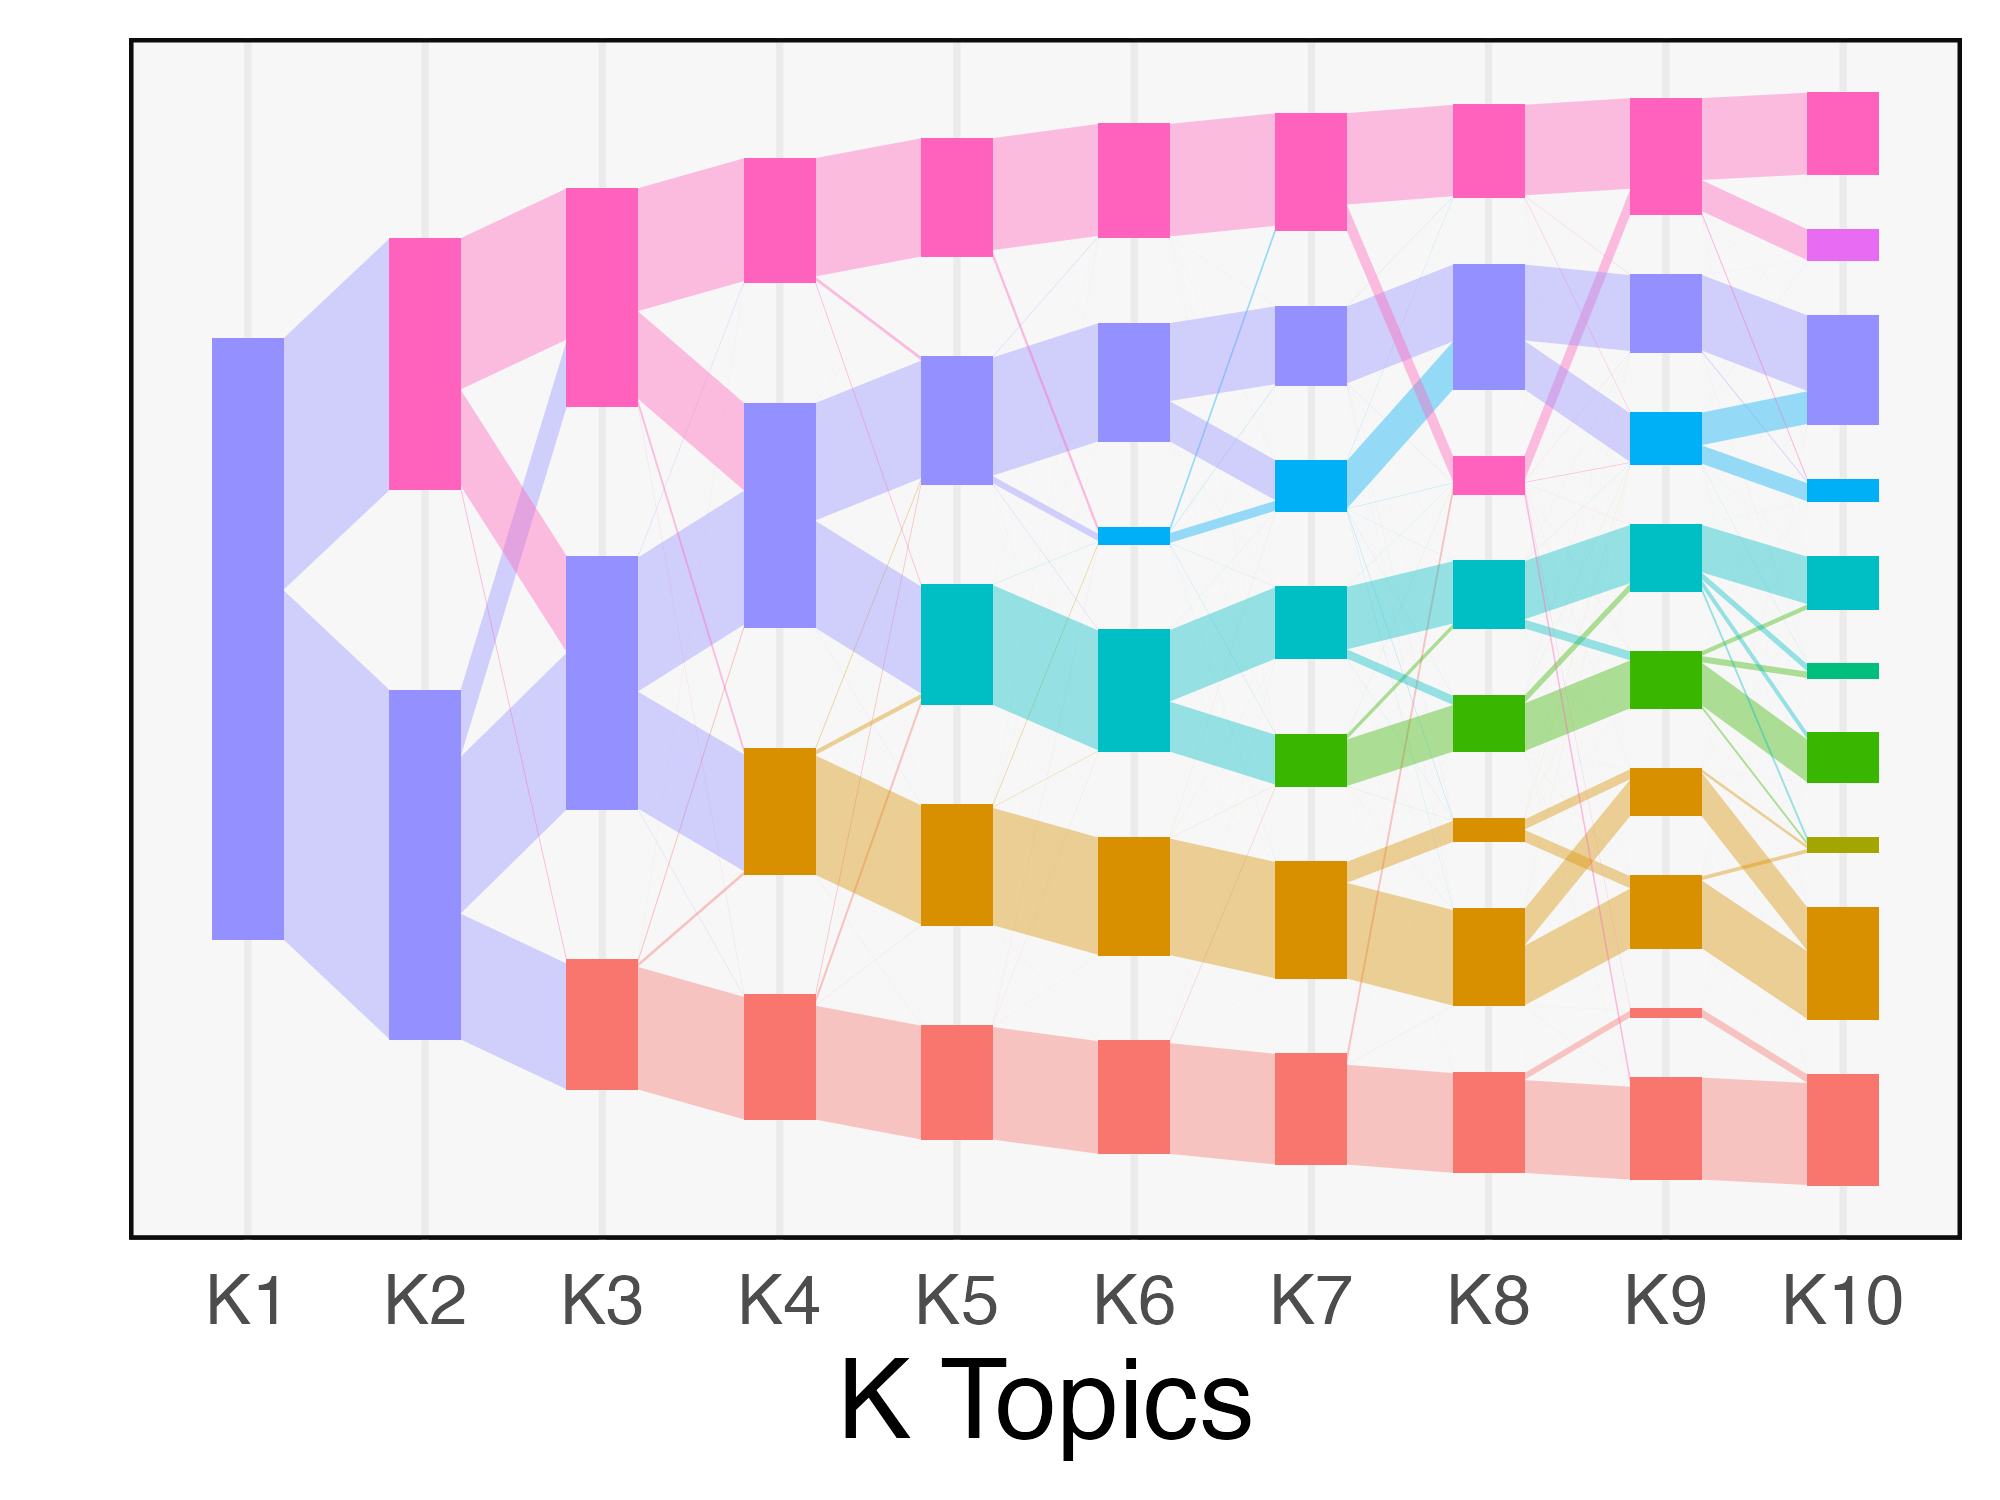
\includegraphics[width=0.35\textwidth]{equivalence_flow}}
  \subfloat{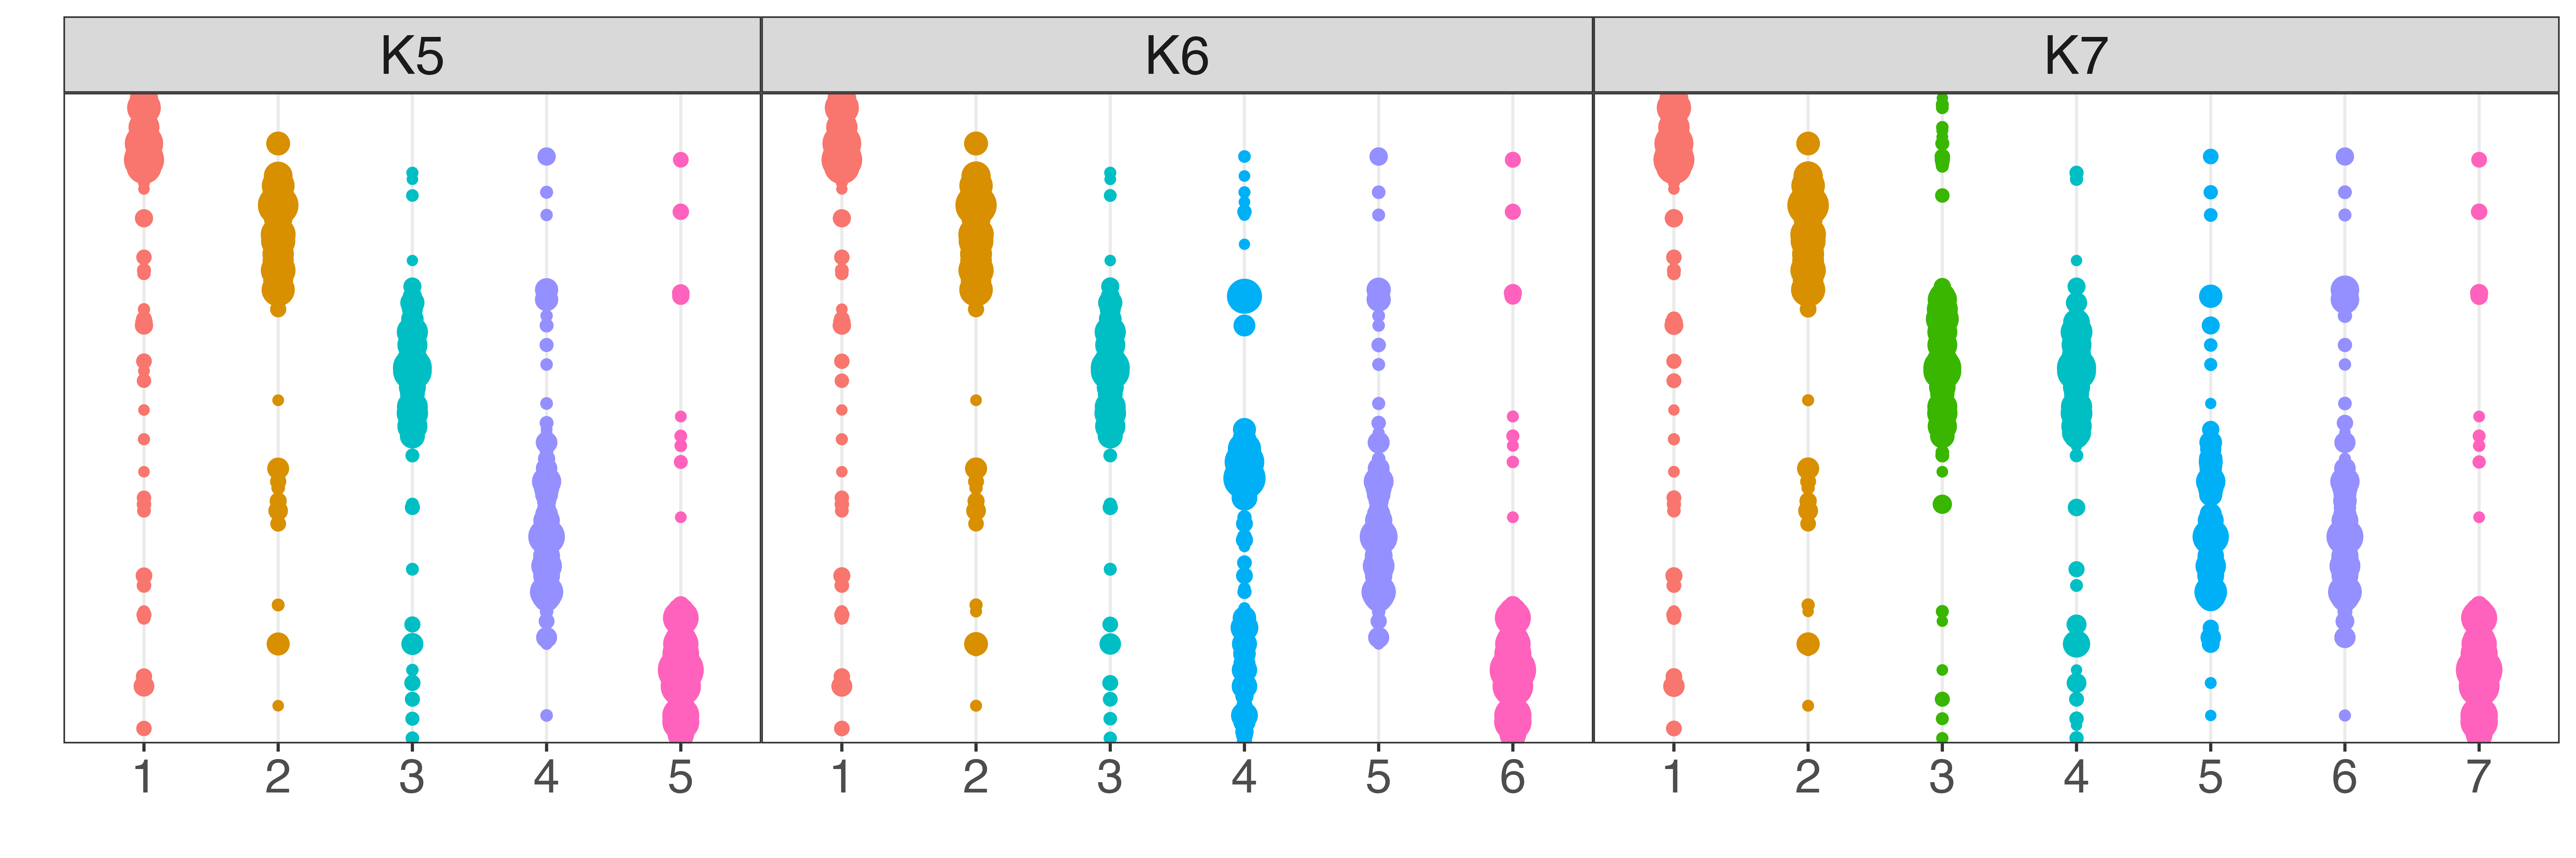
\includegraphics[width=0.63\textwidth]{equivalence_betas}}
\end{figure}

\end{frame}

\begin{frame}
  \frametitle{Results}
  \begin{itemize}
    \item At smaller $K$, we recognize the main community structure, but don't see strain switching
    \item At larger $K$, we are able to recognize instances of switching
  \end{itemize}
\begin{figure}
  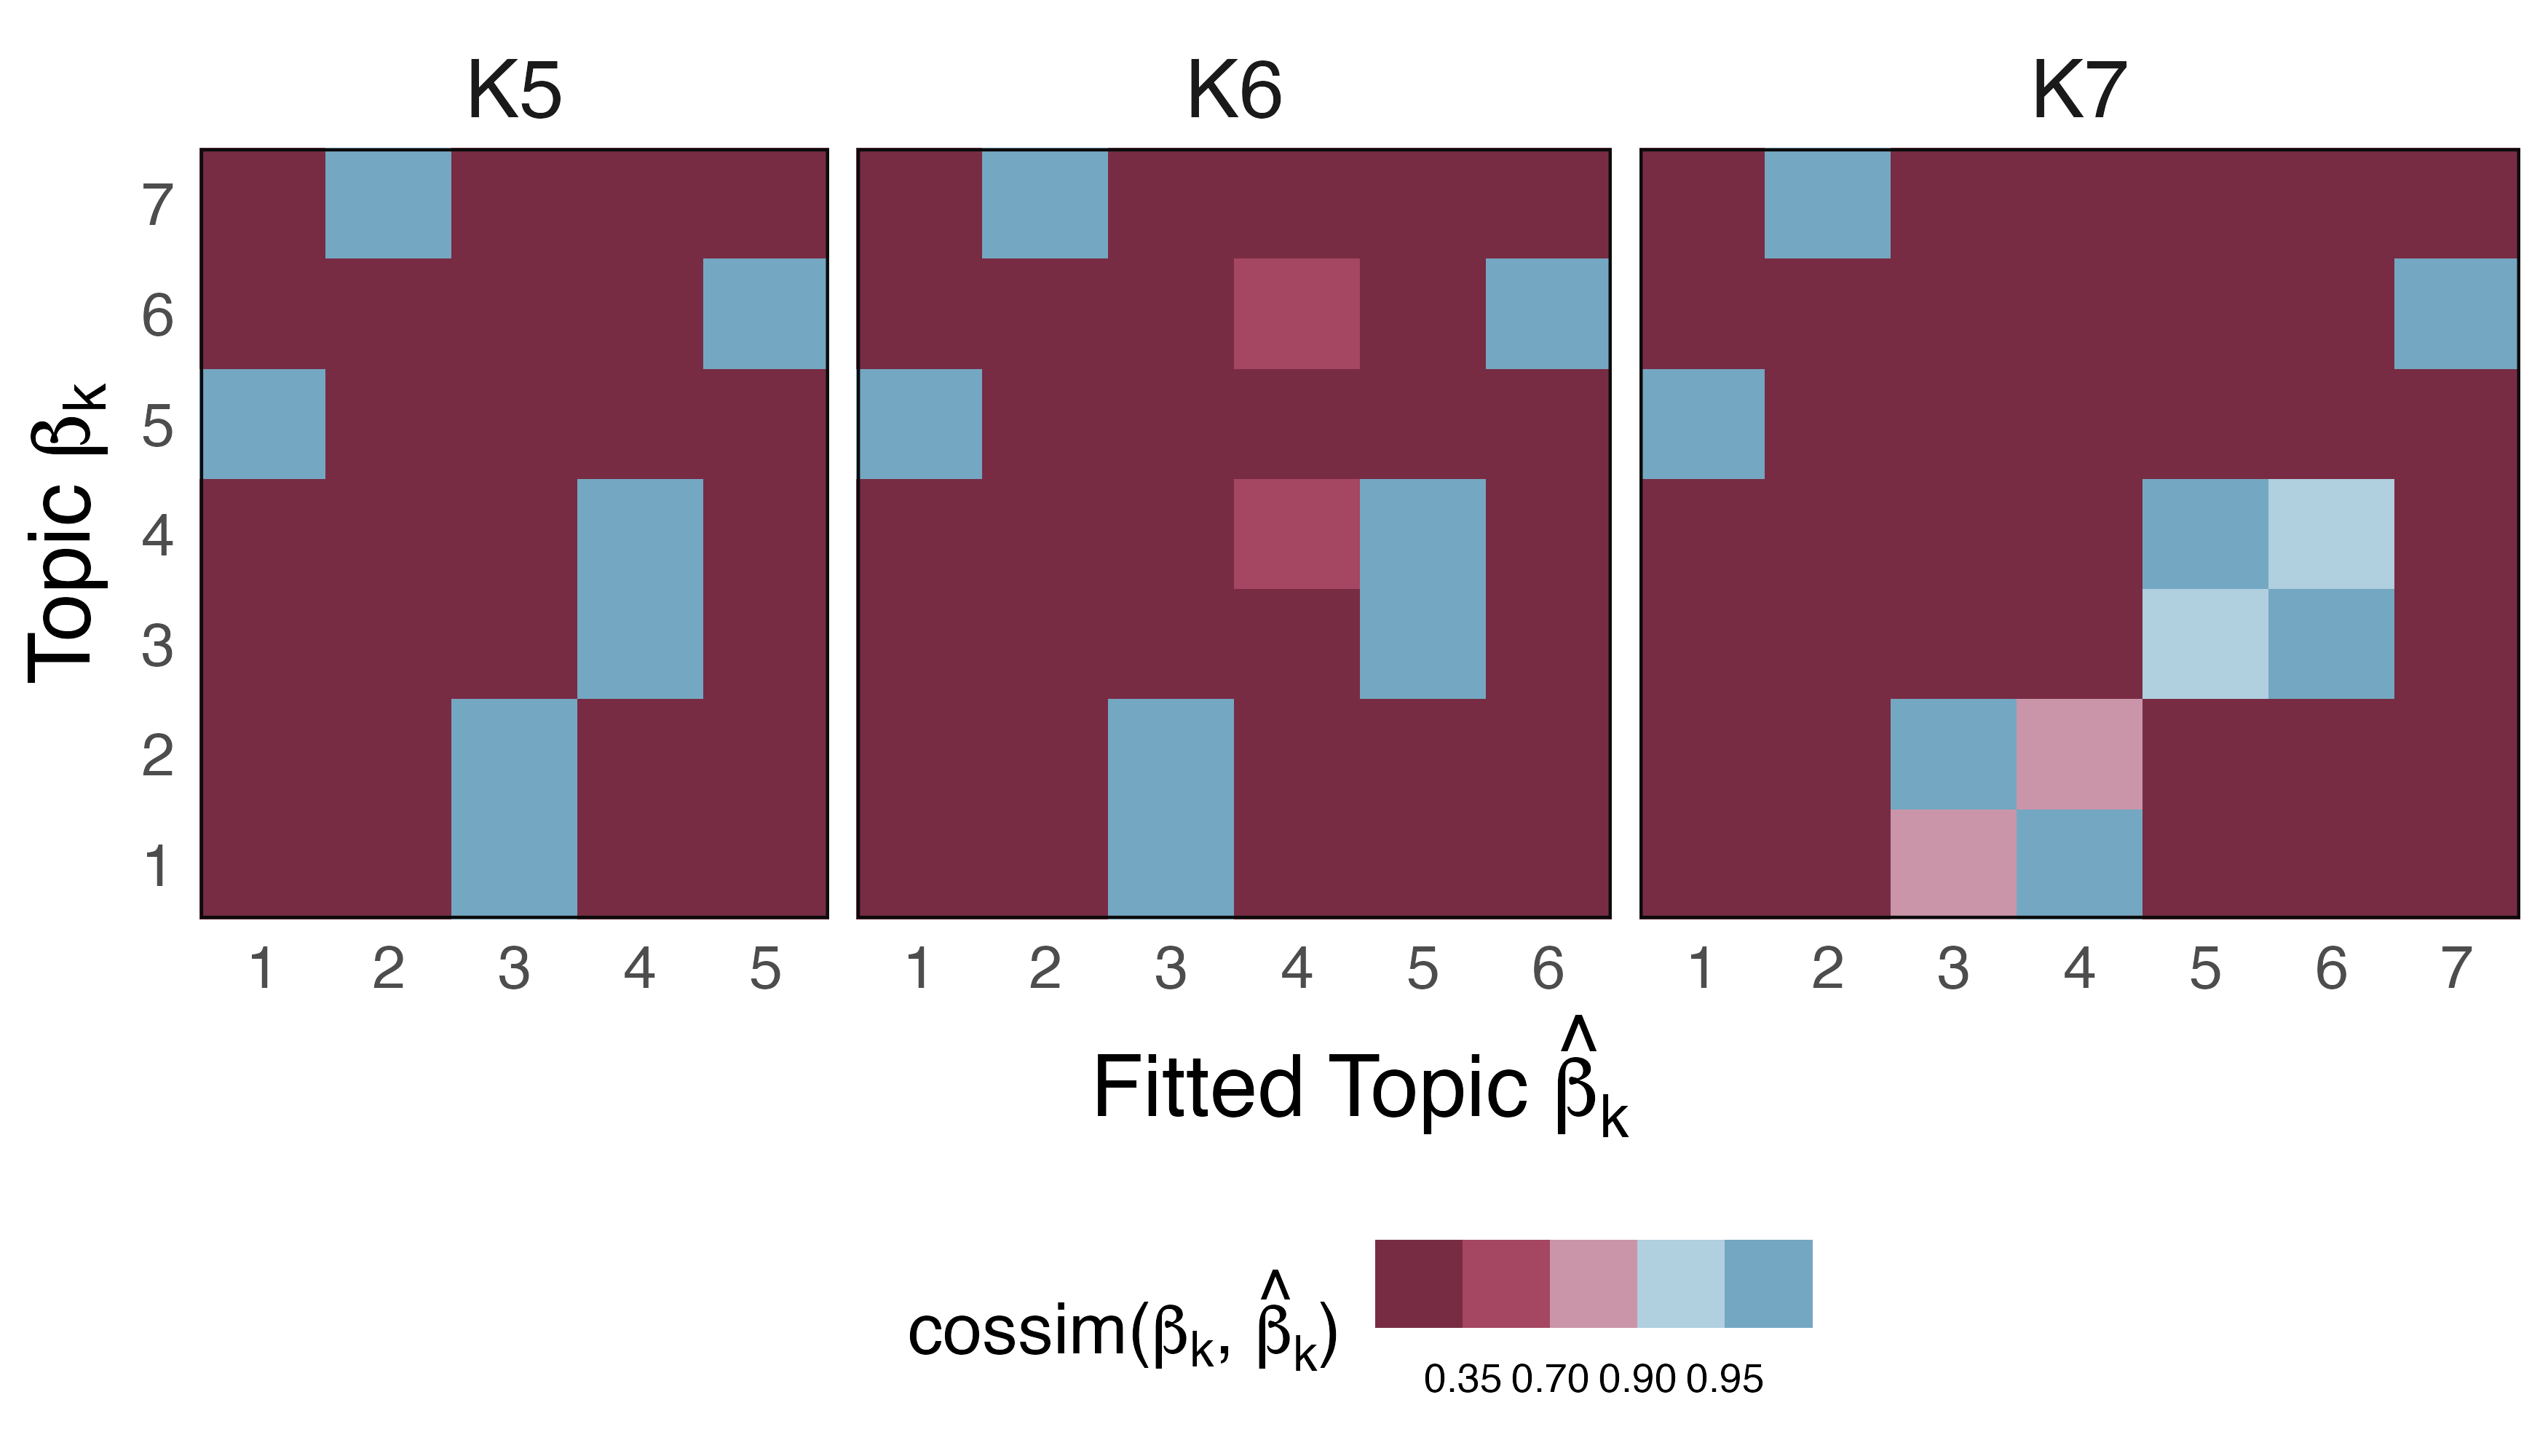
\includegraphics[width=\textwidth]{equivalence_similarity_hm}
\end{figure}
\end{frame}

\section{Data Analysis}

\begin{frame}
  \frametitle{Known structures}
  \begin{itemize}
    \item Historically, the vaginal microbiome has been split into 5 separate
    community state types (CSTs).
    \begin{itemize}
      \item Four are considered healthy, and are each dominated by a Lactobacillus strain
      \item One dysbiotic CST is characterized by lack of a dominant Lactobacillus
    \end{itemize}
  \end{itemize}
\end{frame}


\begin{frame}
  \begin{itemize}
    \item We recover the 4 Lactobacillus Community State Types that have been
    previously documented
    \item Within the dysbiotic CST, we detect 2 consistently different community
    structures
  \end{itemize}
  \begin{figure}
    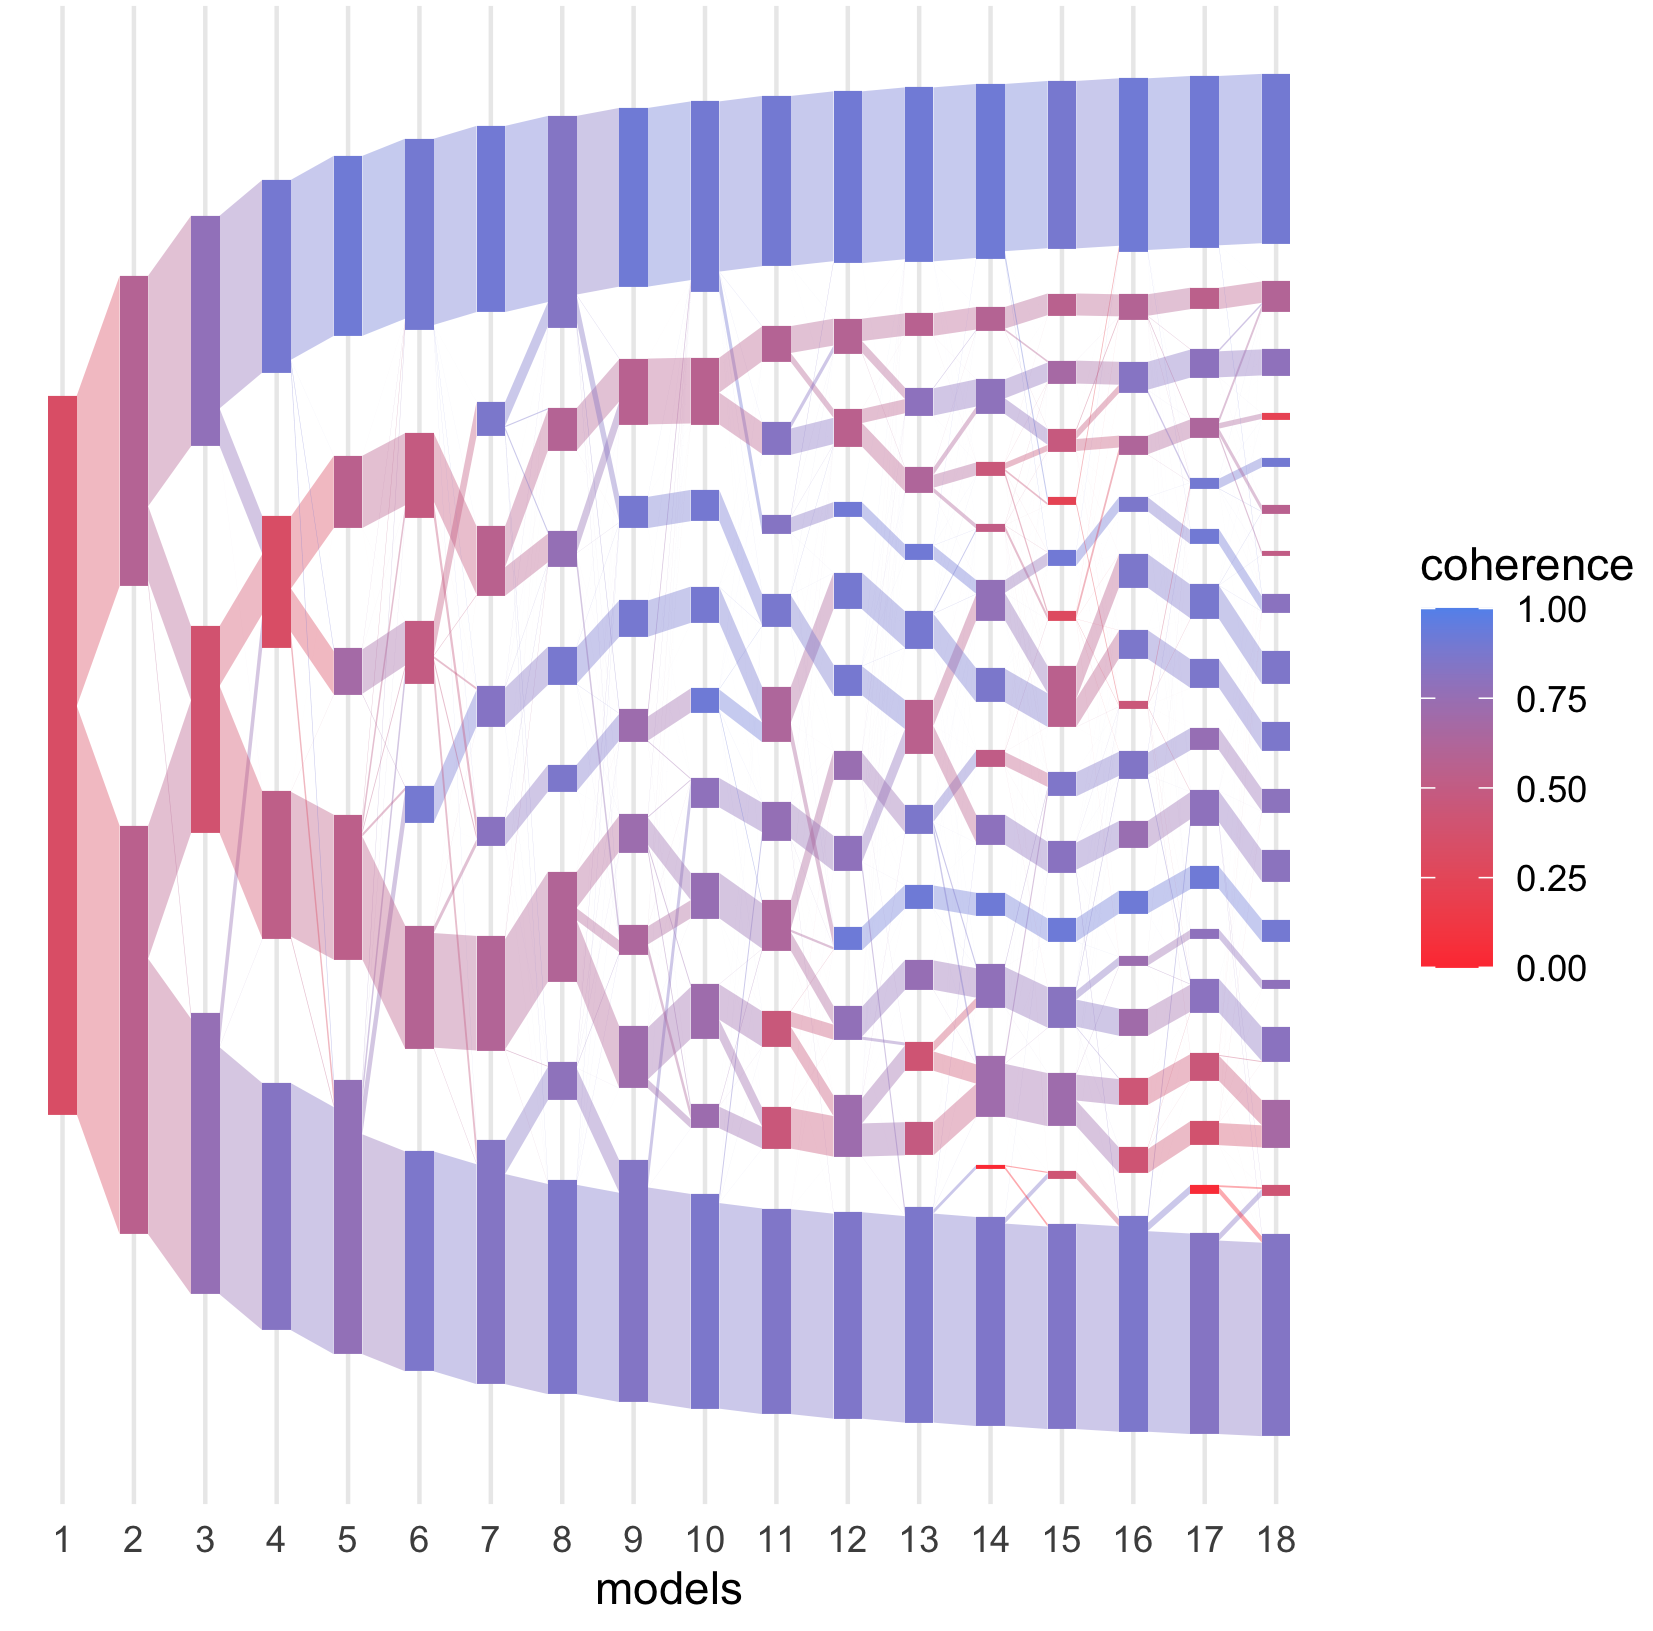
\includegraphics[width=0.7\textwidth]{microbiome_coherence}
  \end{figure}
\end{frame}

\begin{frame}
  \frametitle{Interpretations}
  \begin{itemize}
    \item We recover the 4 Lactobacillus Community State Types that have been
    previously documented
    \item Within the dysbiotic CST, we detect 2 consistently different community
    structures
  \end{itemize}
  \begin{figure}
    \subfloat{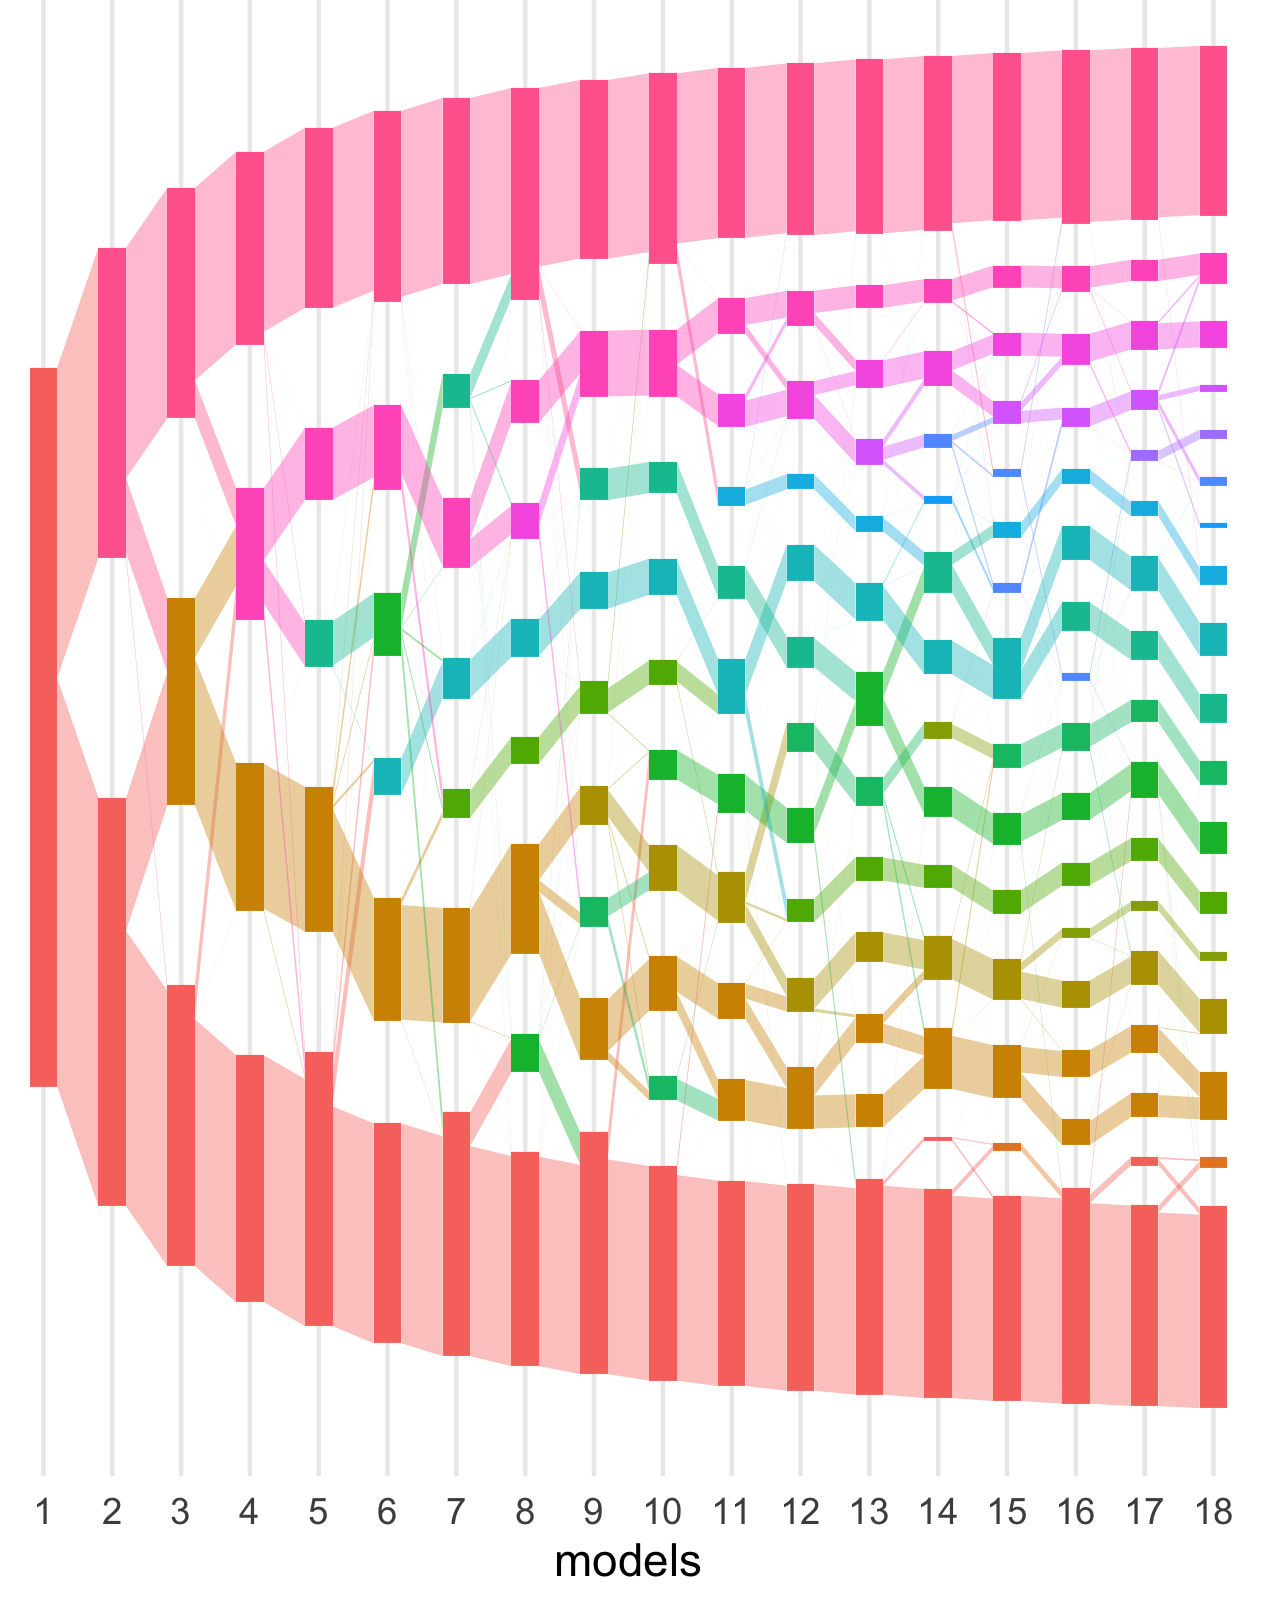
\includegraphics[width=0.35\textwidth]{microbiome_flow}}
    \subfloat{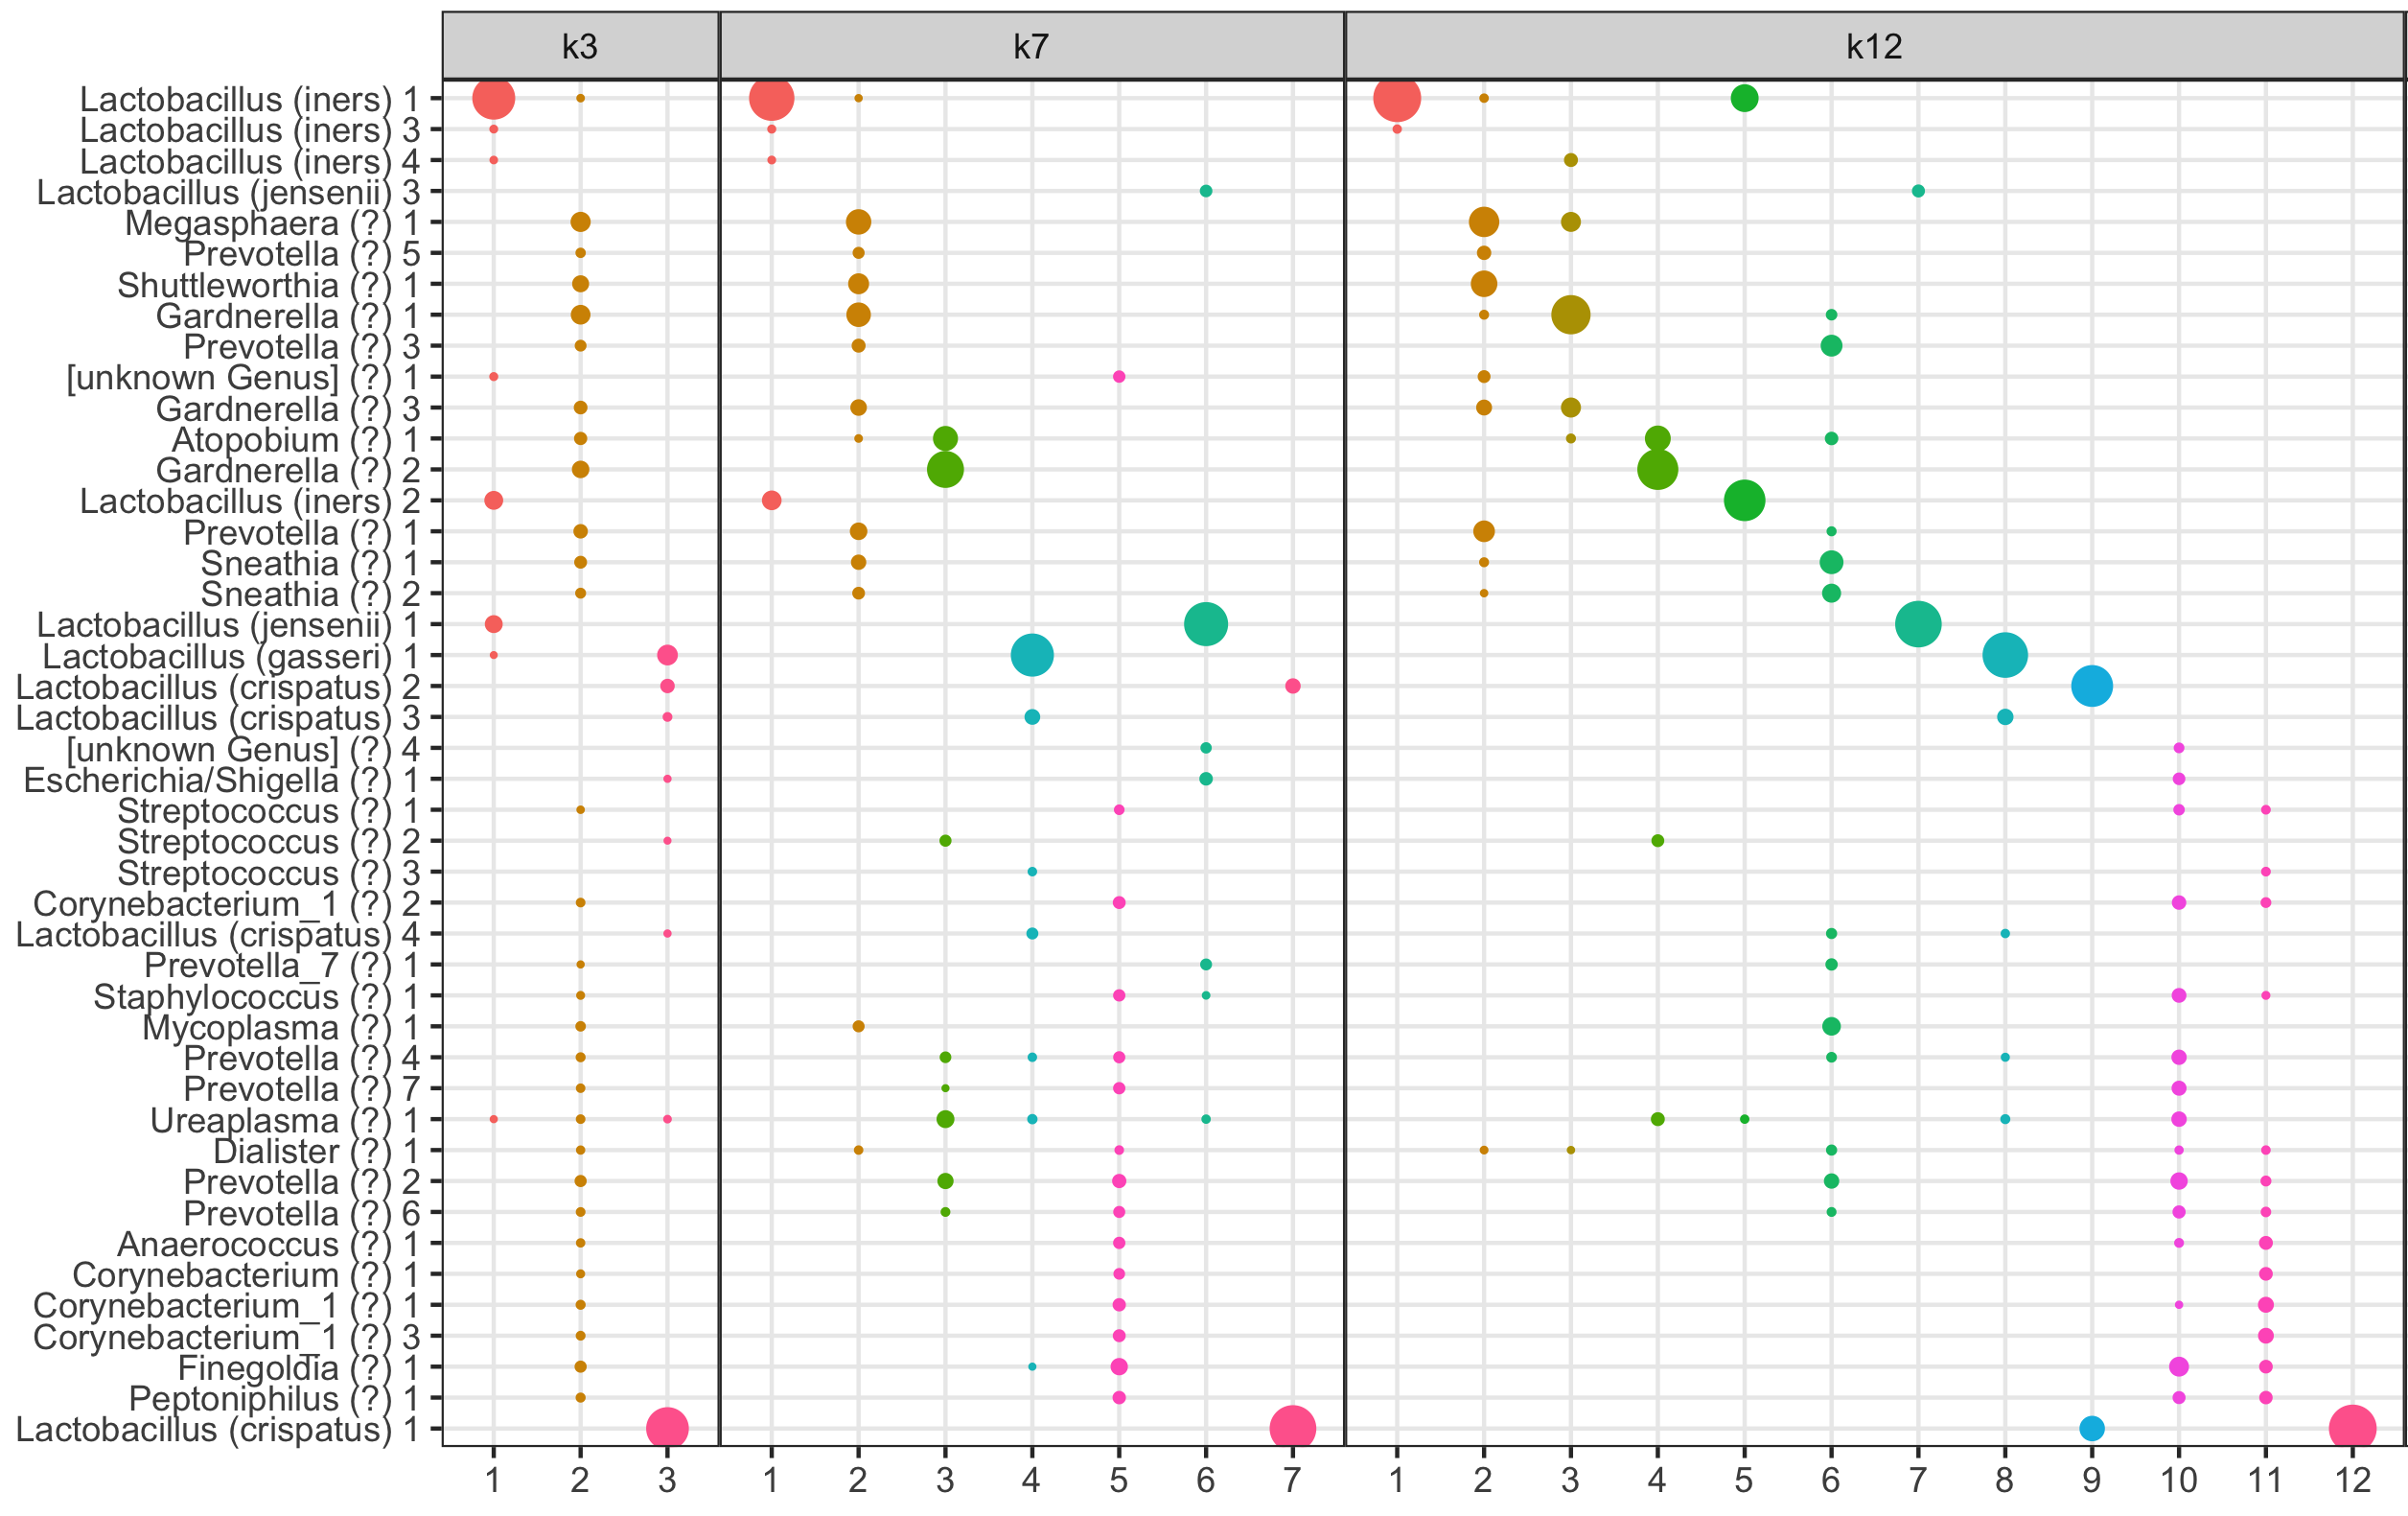
\includegraphics[width=0.63\textwidth]{microbiome_betas}}
  \end{figure}
\end{frame}

\section{Discussion}

\begin{frame}[fragile]
  \frametitle{Software}
    Topic alignment is implemented in the R package
    \href{lasy.github.io/alto}{\texttt{alto}}.

    \begin{lstlisting}
    # simulate data and fit models
    x = rmultinom(20, 5000, rep(0.1, 500))
    lda_params = setNames(map(1:10, ~ list(k = .)), 1:10)
    lda_models = run_lda_models(x, lda_params)

    # perform alignment and plot
    result = align_topics(lda_models)
    plot(result)
    \end{lstlisting}

    All the simulations discussed today are vignettes in the package. (We will
    create a binder link for people to try)
\end{frame}

\section{Topic Alignment}

\begin{frame}
\frametitle{Cognitive Artifacts}
  Why are clustering and dimensionality reduction methods used?

 Human working memory is limited, and these methods provide,
  \begin{itemize}
    \item A compressed representation that is easier to reason about
    \item Guidance of attention to details of interest
\end{itemize}

Both methods create cognitive artifacts that support scientific thinking when
the available data are too much to understand at a glance.
\end{frame}



\section{Analyzing The Hitchhikers of the Rhizosphere (THOR)}

\begin{frame}
  \frametitle{Context}
  THOR is a model microbiome designed by the Handelsman Lab at UW Madison. It
  includes,
  \begin{itemize}
  \item \textit{Pseudomonas koreensis} (a Protobacteria, call this $K$)
  \item \textit{Bacillus cereus} (a Firmicute, call this $F$)
  \item \textit{Flavobacterium johnsoniae} (a Bacteroidetes, call this $B$)
  \end{itemize}
  along with their ``hitchhikers.'' The goal is to understand interactions and
  emergent properties within this controlled system.
\end{frame}

\begin{frame}
  \frametitle{Known Structure}
  The most salient property is that,
  \begin{itemize}
    \item If $K$ and $F$ are left together, then $F$ will die
    \item If $B$ is added to $K$ and $F$ are left together, then $F$ will
    survive
  \end{itemize}

  \begin{figure}
    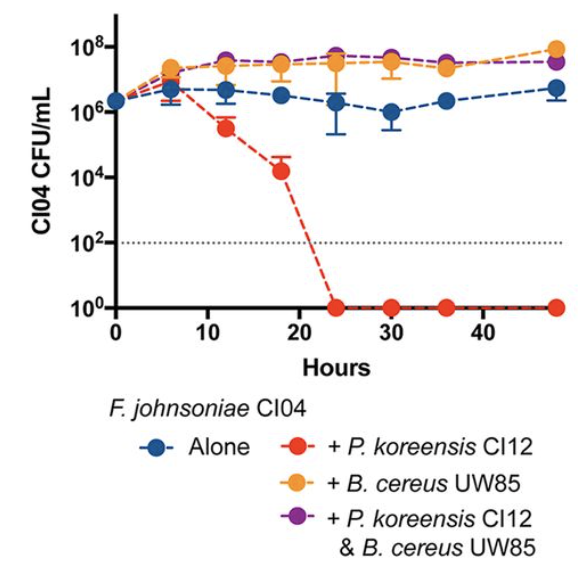
\includegraphics[width=0.4\textwidth]{thor}
  \end{figure}
\end{frame}

\begin{frame}
  \frametitle{Mechanisms}
\begin{itemize}
  \item The first property is caused by $K$'s production of the antibiotic
  koreenceine
  \begin{itemize}
    \item They made a variant of $K$ that couldn't make koreenceine, and $F$ was
    able to survive with this variant present
  \end{itemize}
  \item It's unknown how $B$ protects $F$
  \item The antibiotic also ``hurts'' $K$, even though it's being produced by it
\end{itemize}
\end{frame}

\begin{frame}
  \frametitle{Metabolomics}
  The lab has run LC-MS experiments on the system,
  \begin{itemize}
    \item 3882 metabolites
    \item $2^3$ design (pure media, just $F$, just $FK$, ...)
  \end{itemize}

  \begin{figure}
    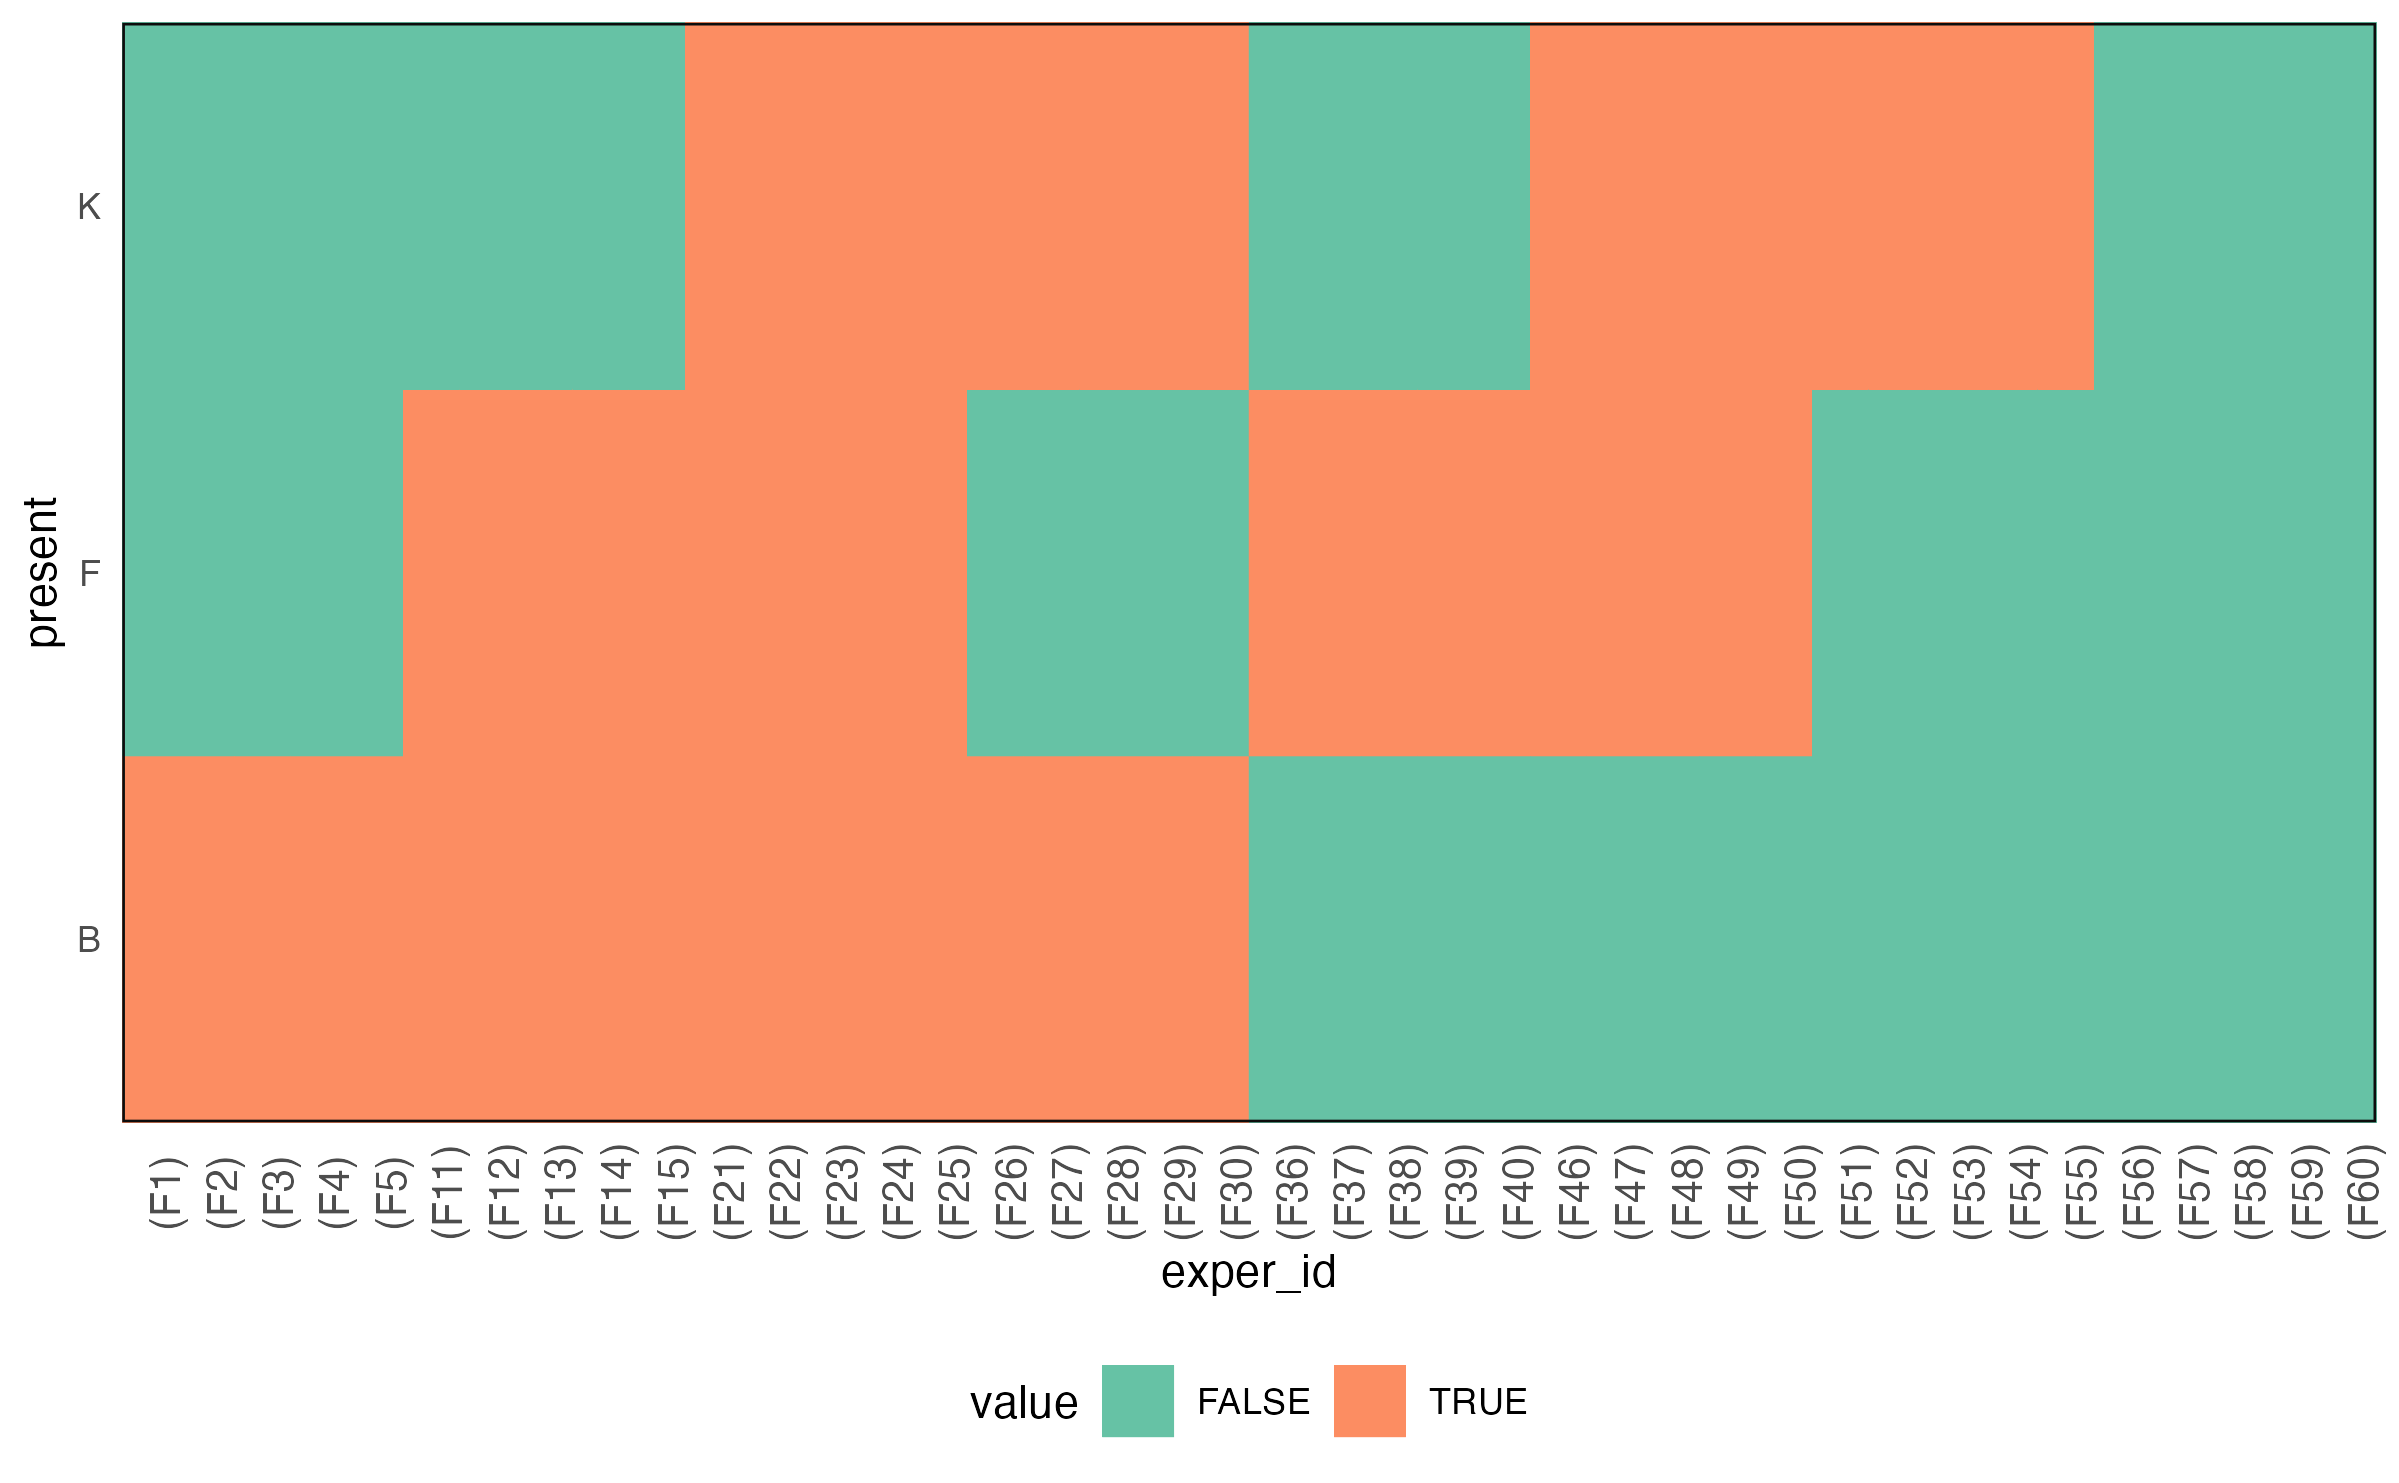
\includegraphics[width=0.8\textwidth]{configurations}
  \end{figure}
\end{frame}

\begin{frame}
  \frametitle{Examples}
    If there were only a couple of metabolites, we would use classical
    (nonparametric?) ANOVA

  \begin{figure}
    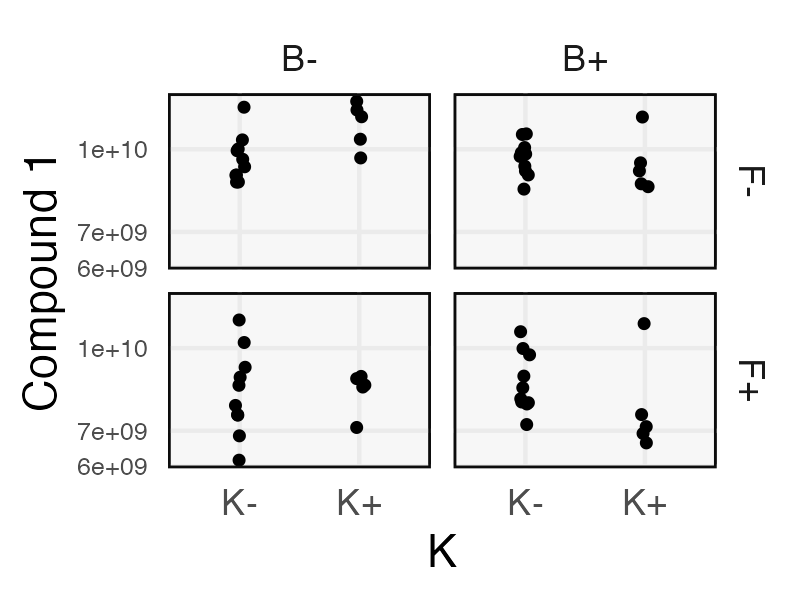
\includegraphics[width=0.4\textwidth]{compound-1}
  \end{figure}

    But since there are many, we should try to (a) guide our search and (b)
    share across sources, somehow.
\end{frame}

\begin{frame}
  \frametitle{Examples}
    If there were only a couple of metabolites, we would use classical
    (nonparametric?) ANOVA
  \begin{figure}
    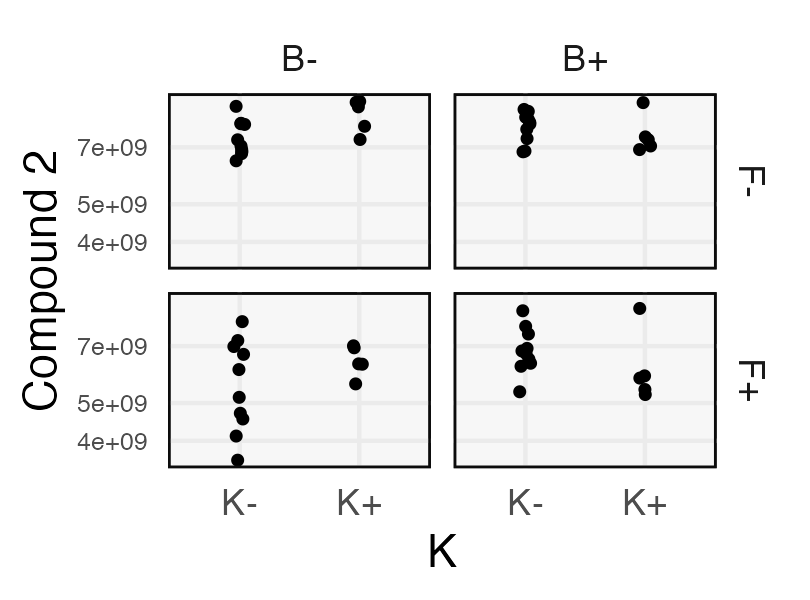
\includegraphics[width=0.4\textwidth]{compound-2}
  \end{figure}

    But since there are many, we should try to (a) guide our search and (b)
    share across sources, somehow.
\end{frame}

\begin{frame}
  \frametitle{Examples}
    If there were only a couple of metabolites, we would use classical
    (nonparametric?) ANOVA
  \begin{figure}
    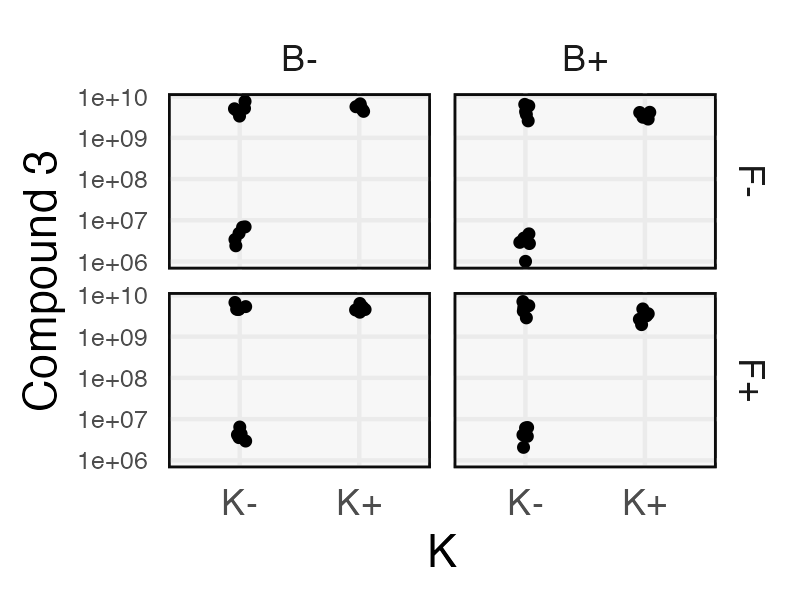
\includegraphics[width=0.4\textwidth]{compound-3}
  \end{figure}

    But since there are many, we should try to (a) guide our search and (b)
    share across sources, somehow.
\end{frame}

\begin{frame}
  \frametitle{Examples}
    If there were only a couple of metabolites, we would use classical
    (nonparametric?) ANOVA
  \begin{figure}
    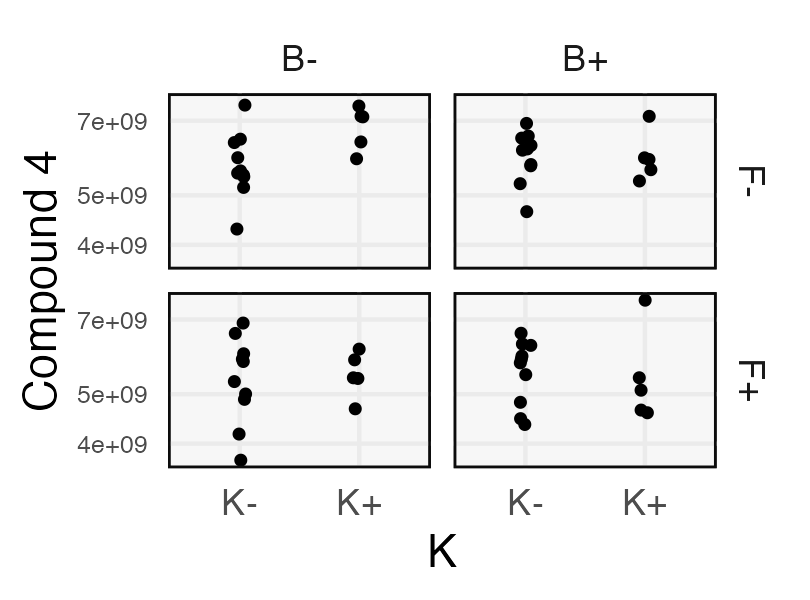
\includegraphics[width=0.4\textwidth]{compound-4}
  \end{figure}

    But since there are many, we should try to (a) guide our search and (b)
    share across sources, somehow.
\end{frame}

\begin{frame}
  \frametitle{Examples}
    If there were only a couple of metabolites, we would use classical
    (nonparametric?) ANOVA
  \begin{figure}
    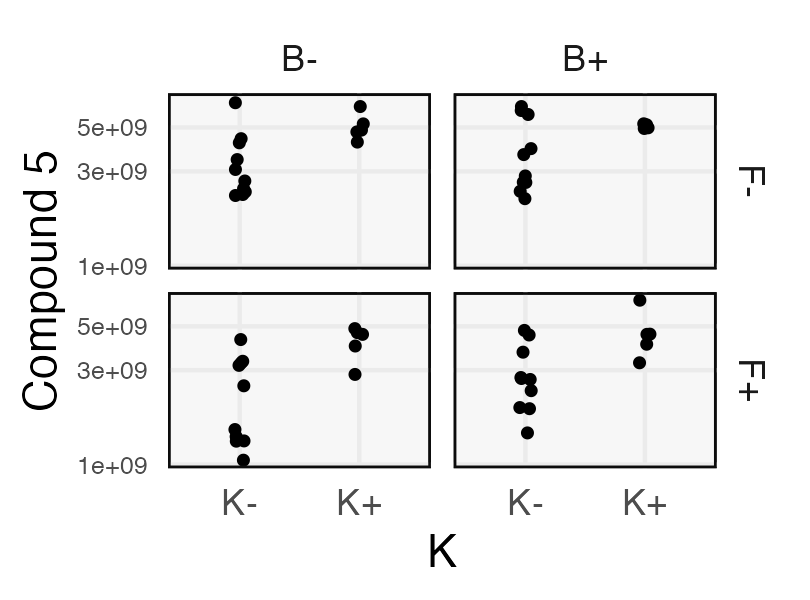
\includegraphics[width=0.4\textwidth]{compound-5}
  \end{figure}

    But since there are many, we should try to (a) guide our search and (b)
    share across sources, somehow.
\end{frame}

\begin{frame}
  \frametitle{Ideas}
  Two overarching data analysis approaches come to mind,
  \begin{itemize}
    \item Summarize and then estimate effects: Learn main patterns among
    metabolites and then see how they differ across conditions
    \item Estimate effects and then summarize: Fit an ensemble of ANOVA models
    and then select / cluster metabolites
  \end{itemize}
  These are analogous to \texttt{diffTop} (or MANOVA) and multiple testing,
  respectively.
\end{frame}

%   lm(log(value) ~ (B + F + K) ^ 2, data = .))
\begin{frame}
  \frametitle{Coefficients}

  These are $t$-statistics of marginal effects from the model,
  \begin{align*}
    \log\left(\text{Compound}\right) &= \beta_0 + \sum_{j \in B, F, K} \beta_{j}x_{j} + \sum_{j, j^\prime \in \{\text{All Pairs}\}} \beta_{jj'}x_{j}x_{j'}
  \end{align*}

  \begin{figure}
    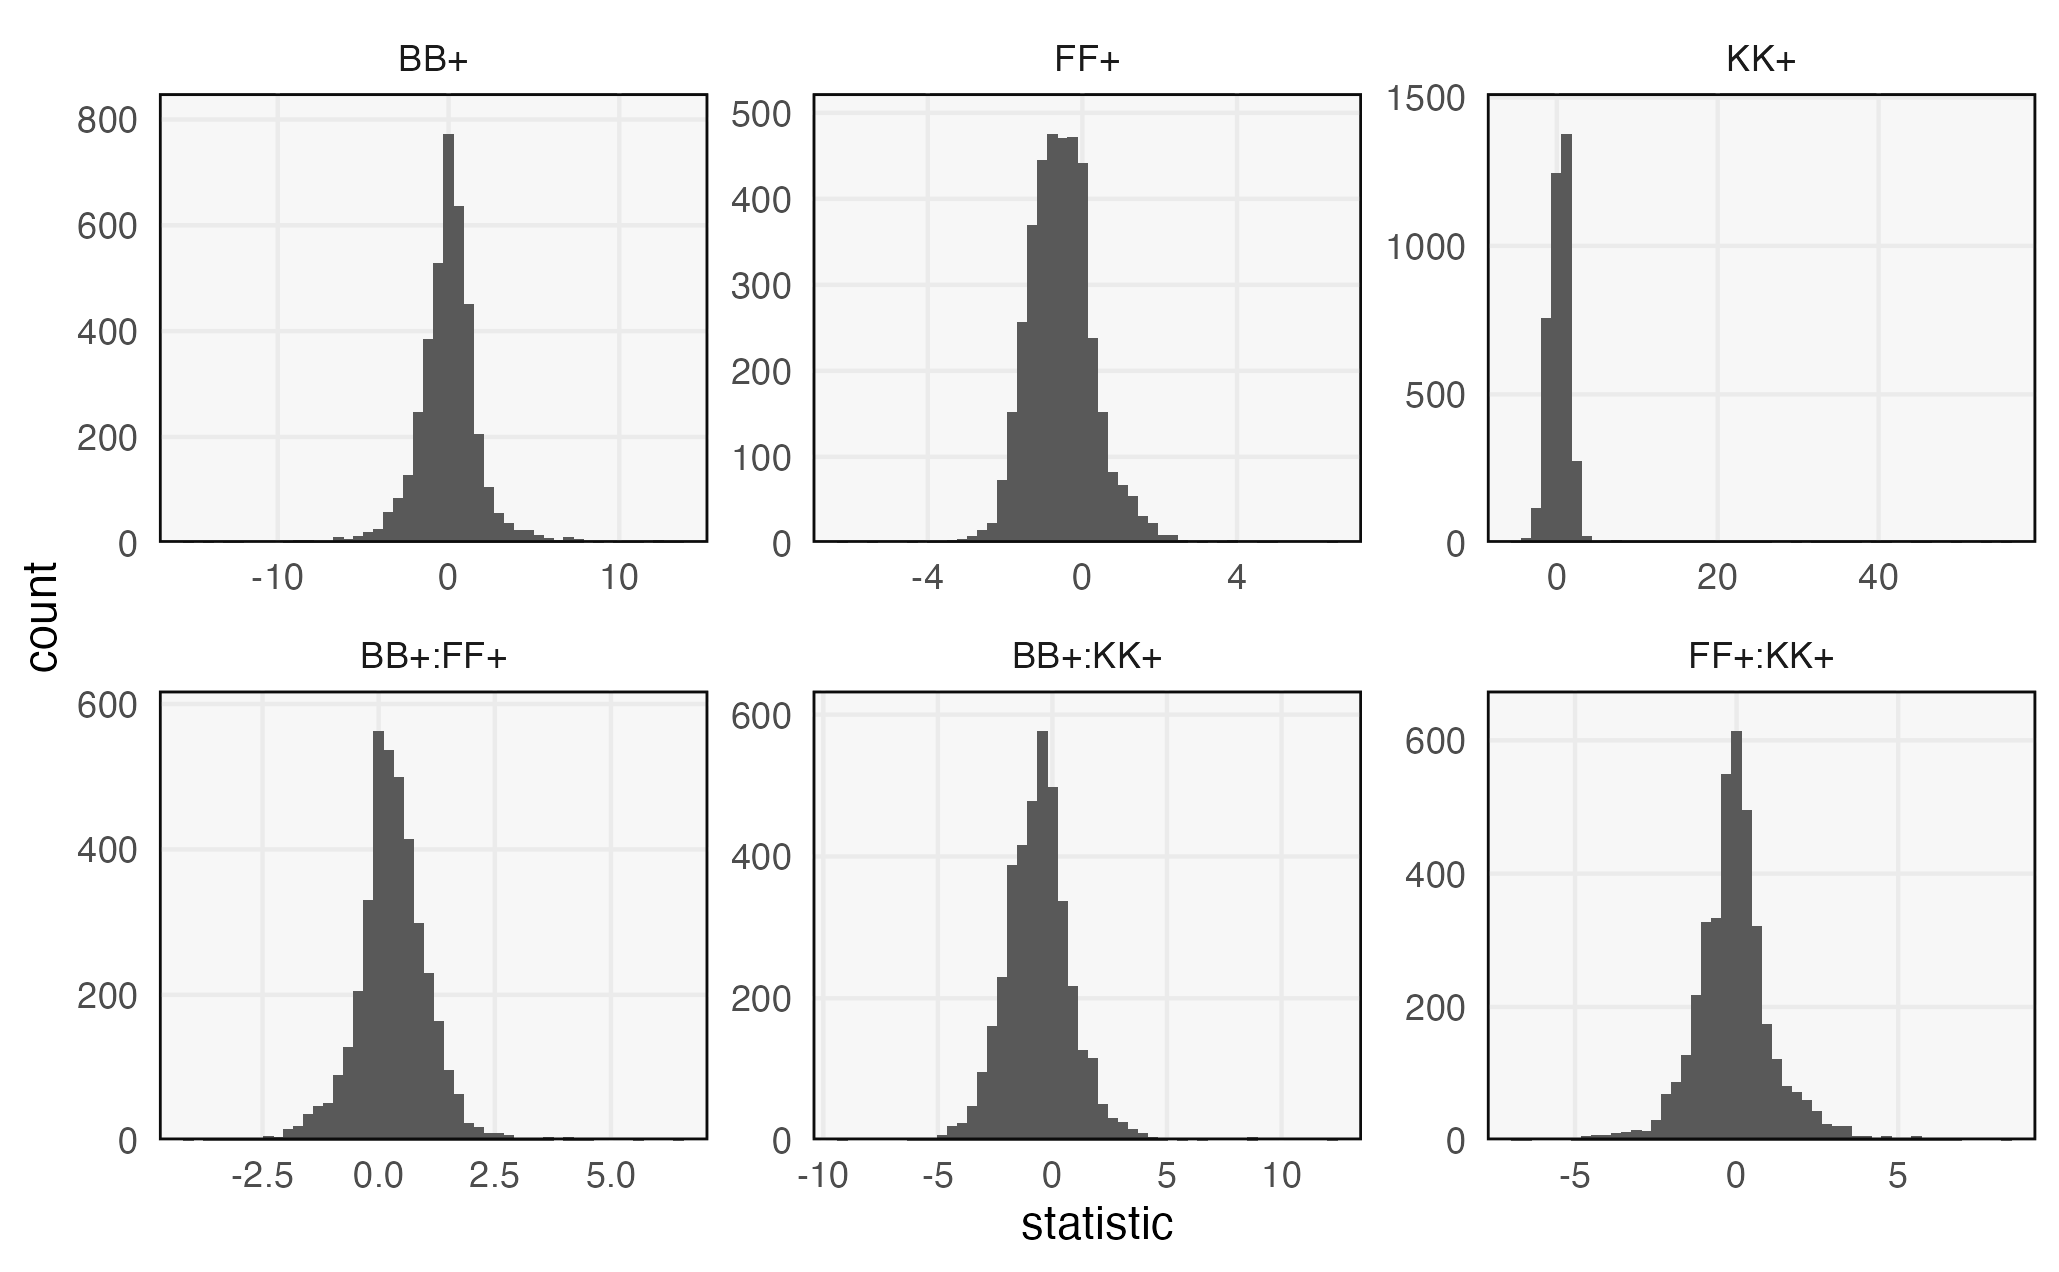
\includegraphics[width=0.7\textwidth]{marginal-coefficients}
  \end{figure}
  Note the varying $x$-scales. The long-tails are significant effects.
\end{frame}

\begin{frame}
  \frametitle{Relationships}
  One of the benefits of simultaneous inference is that we can look the
  relationships between coefficients.

  \begin{figure}
  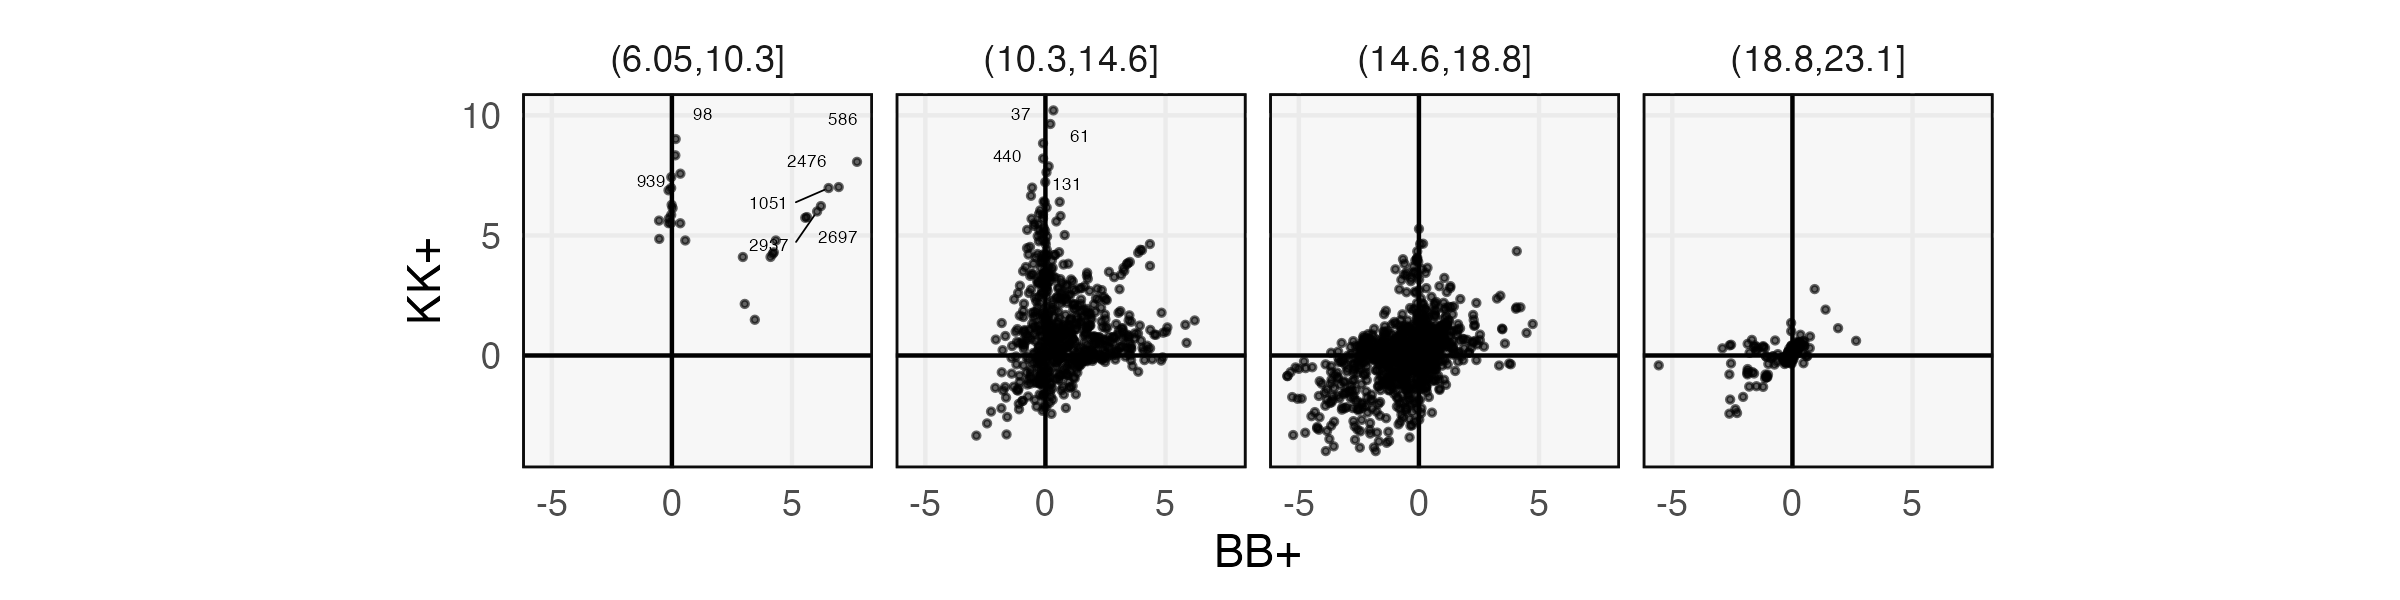
\includegraphics[width=0.8\textwidth]{bk-scatter}
  \end{figure}
\end{frame}

\begin{frame}
  \frametitle{Relationships}
  One of the benefits of simultaneous inference is that we can look the
  relationships between coefficients.

  \begin{figure}
  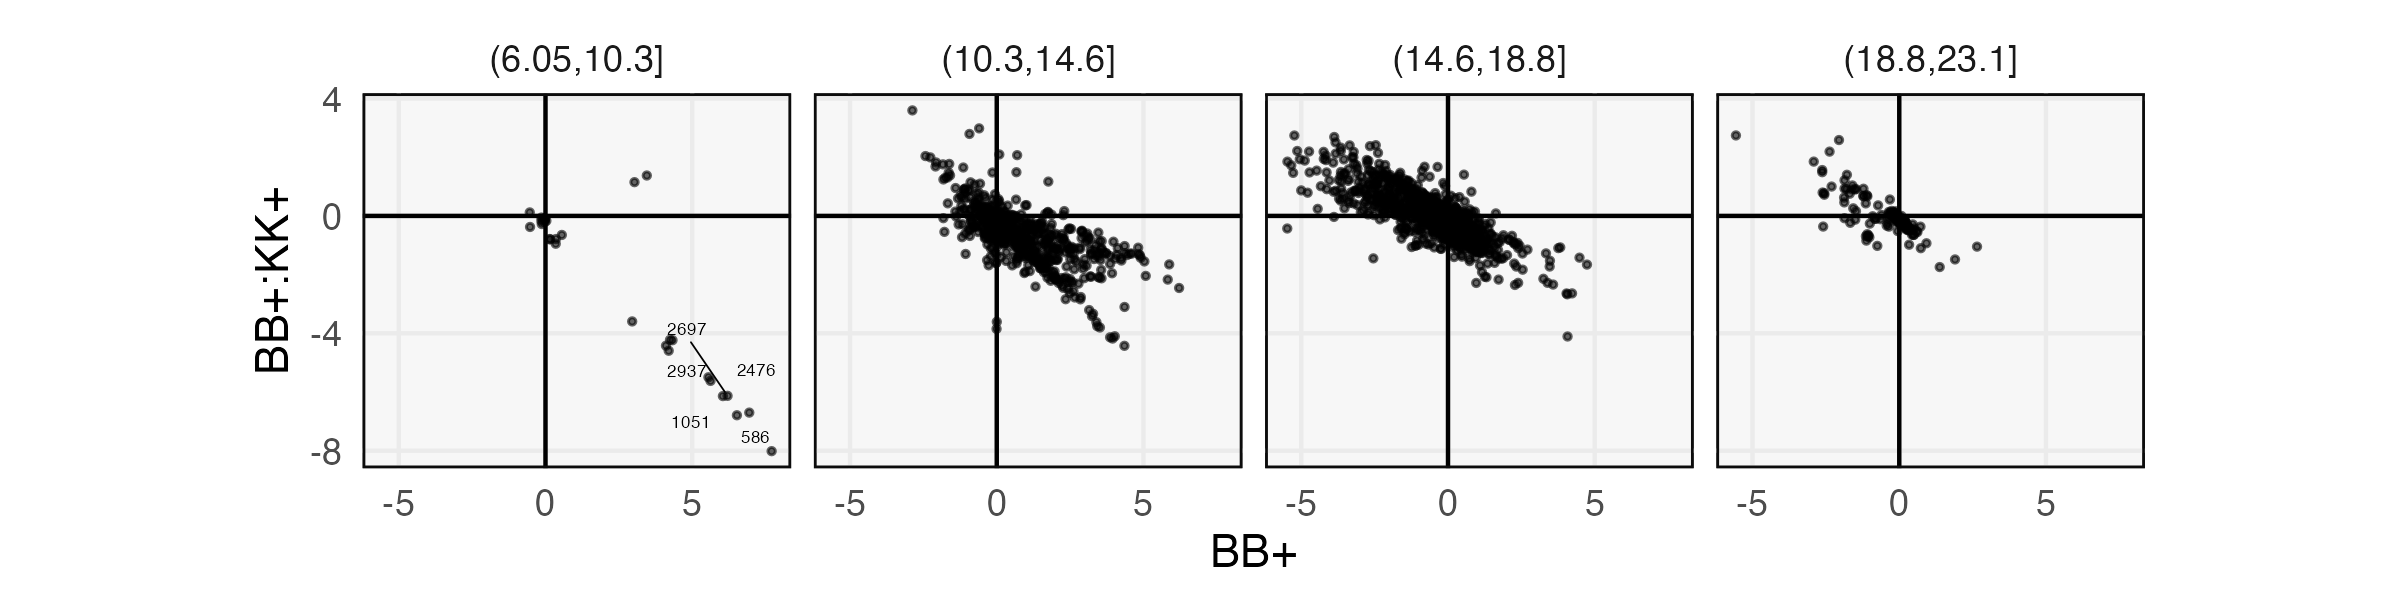
\includegraphics[width=0.8\textwidth]{bbk-scatter}
  \end{figure}
\end{frame}

\begin{frame}
  The hope is that the extremes in these scatterplots suggest interesting
  metabolites for follow-up work. (Ideally, can help people search using
  characteristics of metabolites, too).
  \begin{figure}
    \subfloat{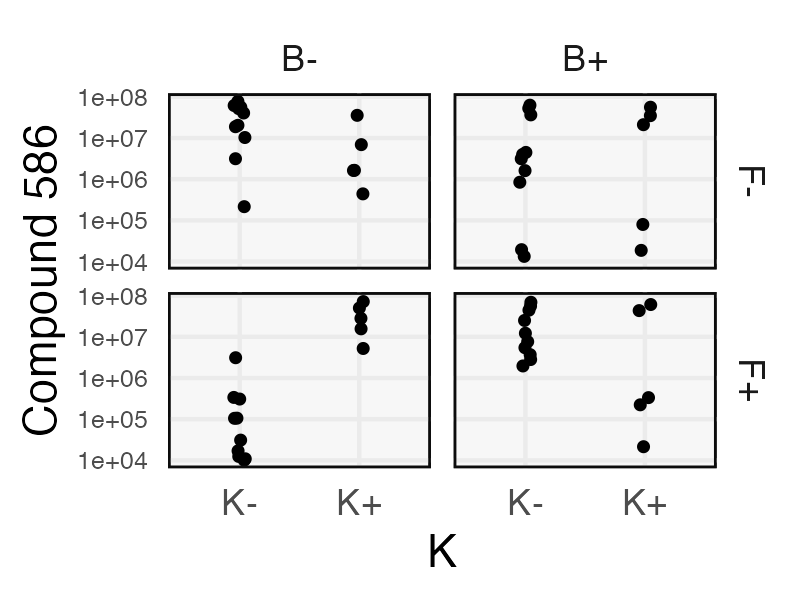
\includegraphics[width=0.4\textwidth]{compound-586}}
    \subfloat{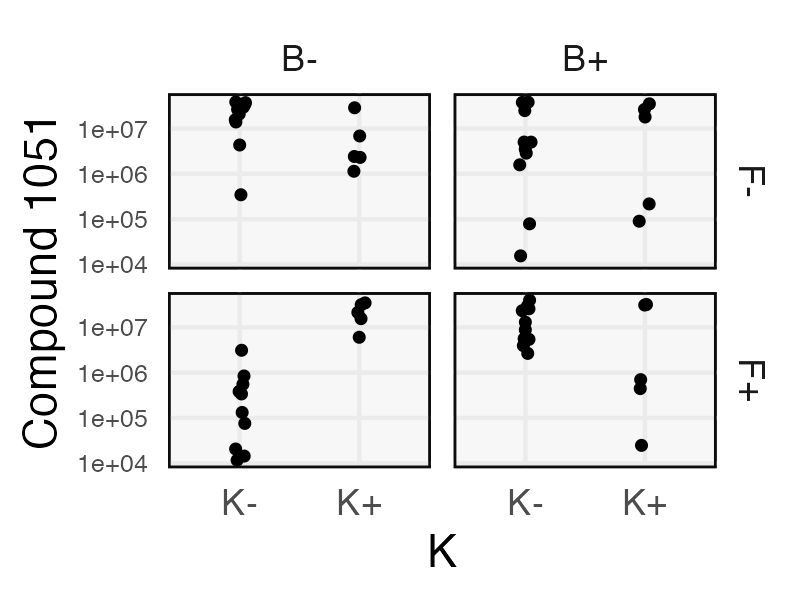
\includegraphics[width=0.4\textwidth]{compound-1051}}
  \end{figure}
\end{frame}

\end{document}
